\documentclass[12pt,a4paper,twoside]{report}

\usepackage[utf8x]{inputenc}
\usepackage[english,hebrew]{babel}

\usepackage{graphicx}
\usepackage{verbatim}
\usepackage{url}
\usepackage{bm}
\usepackage{float}
\usepackage{eqnarray}

\usepackage{tikz}
\usepackage{tkz-euclide}
\usetikzlibrary{positioning,through,calc,intersections,arrows.meta,external}
\tikzexternalize[prefix=tikz/]
\tikzset{>=stealth} % Use stealth arrows
\usetkzobj{all}

\textwidth=155mm
\textheight=235mm
\topmargin=0pt
\headheight=0pt
\oddsidemargin=-5mm
\evensidemargin=5mm
\headsep=0pt
\parindent=0pt
\renewcommand{\baselinestretch}{1.1}
\setlength{\parskip}{0.3\baselineskip plus 1pt minus 1pt}

\graphicspath{{images/}}

\newcommand*{\p}[1]{\textsf{\small #1}}
\newcommand*{\bover}[1]{\bm{\overline{#1}}}
\newcommand*{\erh}[1]{\setlength{\extrarowheight}{#1}}
\newcommand*{\np}{\selectlanguage{english}\newpage\selectlanguage{hebrew}}

%  Less space above chapter title
\makeatletter
\def\@makechapterhead#1{%
  {\parindent \z@ \raggedright \normalfont
    \ifnum \c@secnumdepth >\m@ne
        \centering\huge\bfseries \@chapapp\space \thechapter
        \hspace{.3em}
    \fi
    \Huge \bfseries #1\par\nobreak
    \vskip 20\p@
  }}
\makeatother


%\includeonly{}

\begin{document}

% !TeX root = chapter-1-2-3.tex

\selectlanguage{hebrew}

\thispagestyle{empty}

\begin{center}
\textbf{\LARGE בחינות בגרות במתמטיקה: החוויה}

\bigskip
\bigskip

\textbf{\LARGE אלגברה והסתברות}

\bigskip
\bigskip
\bigskip
\bigskip

\textbf{\Large מוטי בן-ארי}

\bigskip
\bigskip

\url{http://www.weizmann.ac.il/sci-tea/benari/}
\end{center}

% !TeX root = construct.tex

\begin{center}
\begin{bfseries}
\bigskip
\bigskip

Version 2.1

\bigskip

\today

\end{bfseries}
\end{center}


\vfill

\selectlanguage{english}

\begin{footnotesize}
\begin{center}
\copyright{}\ 2017--19 by Moti Ben-Ari.
\end{center}

This work is licensed under the Creative Commons Attribution-ShareAlike 3.0 Unported License. To view a copy of this license, visit \url{http://creativecommons.org/licenses/by-sa/3.0/} or send a letter to Creative Commons, 444 Castro Street, Suite 900, Mountain View, California, 94041, USA.
\end{footnotesize}

\bigskip

\begin{center}

\includegraphics[width=.15\textwidth]{../../by-sa.png}
\end{center}

\np
\thispagestyle{empty}
\mbox{}
\np
\thispagestyle{empty}

\tableofcontents
\np

\section*{הקדמה}
\addcontentsline{cot}{section}{הקדמה}

מתמטיקאים ידועים לשמצה כי הם מפרסמים והוכחות מסודרות וברורות, ומסתירים את העובדה שסל הניירות שלהם מלא עד אפס מקום בניסיונות שהובילו למבואות סתומים וטעויות. ההיעדר של 
\textbf{תהליכי}
הפתרון עלול לתסכל תלמידים שמתייאשים כאשר הם לא מצליחים לפתור בעיות בניסיון הראשון. לא חסרים פתרונות של בחינות הבגרות, אבל גם הם "נקיים" ללא ניסיונות שלא צלחו ודיונים על דרכי החשיבה שהובילו לפתרונות.

מסמך זה מכיל פתרונות לשאלות  
$1,2,3$
)תנועה והספק, סדרות, הסתברות( של הבחינות 
$806$
בשנים תשע"ד עד תשע"ח עם תיאורים של חוויותי בחיפוש פתרונות.

בסוף כל פרק רשמתי המלצות שגיבשתי לאורך העבודה.
\subsection*{תנועה והספק}

הצעה של אביטל אלבוים-כהן כיוון אותי לפתח את הפתרון של הבעיות ההלו באמצעות תרשימים דו-ממדיים. מצאתי שהתרשימים מאוד עוזרים בזיהוי הקשרים בין קטעי התנועה ובכתיבת הנוסחאות. ניתן להיעזר בתרשימים דו-ממדיים גם בבעיות הספק שיש להן מבנה דומה לבעיות תנועה. התרשימים קלים מאוד לציור ומועילים גם אם קני המידה בכלל לא מדוייקים, כך שניתן להשתמש בהם כאשר פותרים בחינות.


בתרשימים הציר האופקי הוא ציר הזמן והציר האנכי הוא ציר המרחק בבעיות תנועה וציר העבודה בבעיות הספק. היתרון של ייצוג זה הוא שמהיריות וההספקים מוצגים כשיפועים של הקווים. ככל שהמהירות או ההפסק גבוה יותר, הקו תלול יותר. לכל דמות )מכונית, סירה, צבע, וכדומה( ציירתי קו עבור כל קטע בתנועה או בעבודה. בבעיות תנועה, יש לשים לב שבניגוד לתרשימים חד-ממדיים בהם אורך קו הוא מרחק הנסיעה, כאן מרחק הנסיעה הוא ההפרש בציר האנכי בין הנקודה ההתחלתית לנקודה הסופית.

אני ממליץ על המאמר "פתרונות שונים לבעיות הספק באמצעים גרפיים" מאת אביטל אלבוים-כהן וג'ייסון קופר. על"ה גיליון
$51$,
מרץ
$2015$,
עמ'
$14$-$19$.
הם מביאים פתרונות גיאומטריים עבור בעיות הספק.

\subsection*{סדרות}

לדעתי, שאלות הסדרות הן הכי קלות לפתור, כדי בסופו של דבר יש יחסים ברורים בין איברים עוקבים בסדרה )חשבונית או הנדסית(, וכן בין האיברים לסכומם. עם זאת, מצאתי שקל מאוד לטעות, למשל, אם מבלבלים בין האינדקסים של איברי הסדרה לבין ערכיהם.

חשבו לשים לב שתת-סדרה של סדרה חשבונית / הנדסית לא "יורשת" את התכונה חשבונית / הנדסית, להיפך, סדרה הבנוייה מתת-סדרות חשבוניות / הנדסיות אינה בהכרח סדרה שהיא חשבונית / הנדסית.

לפני שניגשים לפתרון של שאלה עם סדרה באורך
$n$,
כדאי לרשום וחשב סדרה עם מספר קטן של איברים. כך אפשר לקבל תחושה של היחסים בין איברי הסדרה, ונוסף, זה עוזר כדי להבין מתי לסדרה יש מספר זוגי של איברים ומתי יש מספר אי-זוגי של איברים.

\np

\subsection*{הסתברות}

החישובים בבעיות עם הסתברות הם בדרך כלל פשוטים, אבל קשה יחסית לתרגם את העלילה המילולית למשוואות הנכונות. הדבר נכון במיוחד כאשר השאלה שואלת על הסתברות מותנית. מצאתי עושר רב של ביטויים המכוונים להסתברות מותנית )סיכמתי אותם בסעיף ההמלצות(, וזה לא מקל על הפתרון.

קושי נוסף נובע מהעובדה שיש שתי דרכים שונות לארגן את המידע הנתון והחישובים: בטבלה או בעץ. שאלה על משהו שהוא "גם א וגם ב" מכוון לחיתוך של הסתברויות, ומכוונת לטבלה, לעומת שאלה המנוסחת "א ואחר כך ב" מכוונות למכלפה של הסתברויות הכדאי להציג בעץ. ככל שפותרים יותר שאלות, 
קל יותר להבחין באפיונים של הבעייה ובחור את הדרך הנכונה למצוא פתרון.


\selectlanguage{english}

\tikzsetfigurename{motion}
% !TeX root = bagrut-806.tex

\selectlanguage{hebrew}

\chapter{תנועה והספק}

%%%%%%%%%%%%%%%%%%%%%%%%%%%%%%%%%%%%%%%%%%%%%%%%%%%%%%%%%%%%%%%%

\section{קיץ תשע"ח מועד ב}

\begin{center}
\selectlanguage{english}
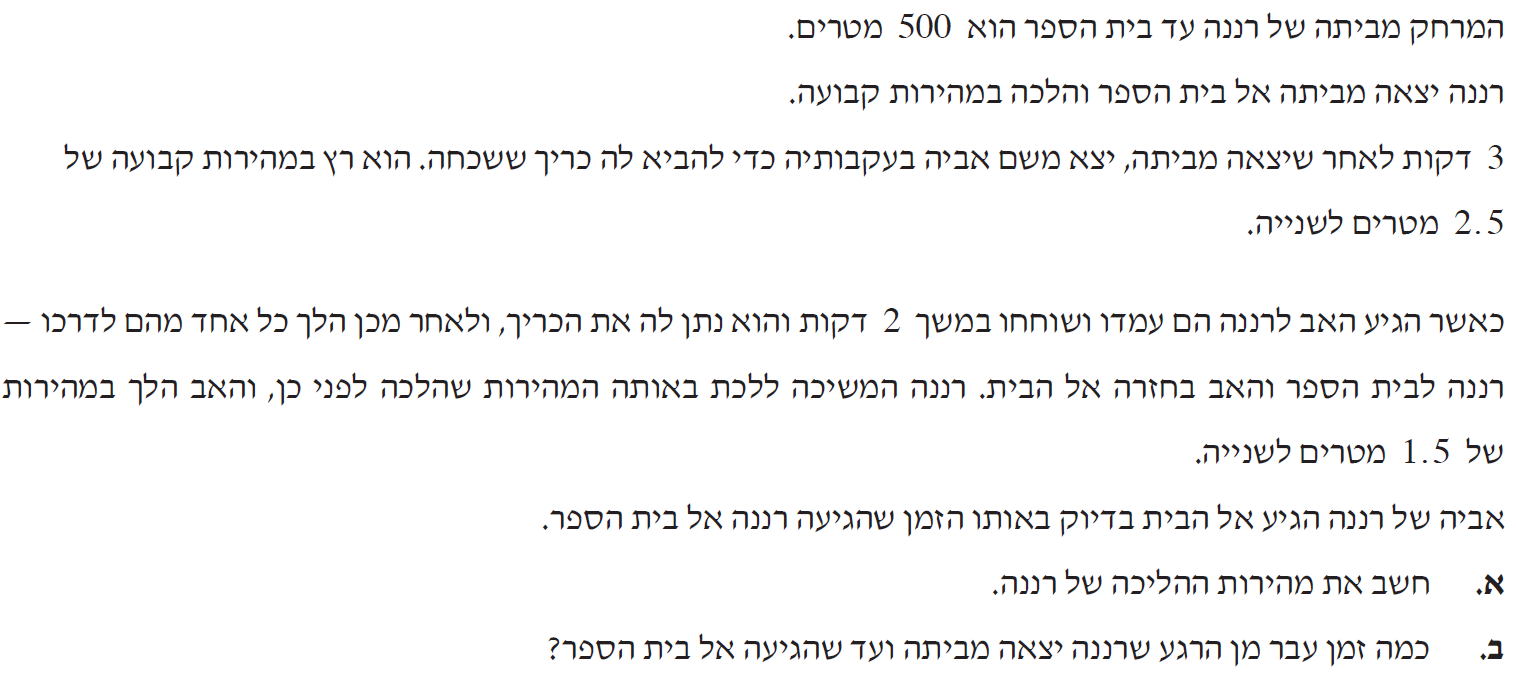
\includegraphics[width=\textwidth]{summer-2018b-1}
\end{center}

\begin{center}
\selectlanguage{english}
\begin{tikzpicture}
\draw (0,0) node[left] {$0$ } -- (10,0);
\node at (-.45,0.5) {
\R{בית}
};
\draw (0,0) -- (0,6) node[left] {$500$};
\node at (-.84,5.5) {
\R{בית ספר}
};
\draw[dashed] (0,6) -- (10,6);
\draw[thick] (0,0) -- node[above left] {
\R{רננה}
} (4.5,3);
\draw[thick] (2,0) -- node[above right,xshift=10pt,near start] {
\R{אבא}
} (4.5,3);
\draw[thick] (4.5,3) -- node[above] {
\R{רננה ואבא}
} (7,3);
\draw[thick] (7,3) -- node[above right] {
\R{אבא}
} (10,0);
\draw[thick] (7,3) -- node[above left] {
\R{רננה}
} (10,6);
\fill (4.5,3) circle [radius=2pt];
\fill (0,0) circle [radius=2pt];
\fill (2,0) circle [radius=2pt];
\fill (4.5,0) circle [radius=2pt];
\fill (7,0) circle [radius=2pt];
\fill (7,3) circle [radius=2pt];
\fill (10,0) circle [radius=2pt];
\fill (10,6) circle [radius=2pt];
\draw[dashed] (10,6) -- (10,0);
\draw[dashed] (4.5,3) -- (4.5,0);
\draw[dashed] (7,3) -- (7,0);
\draw[<->] (0,-5mm) -- node[fill=white] {$180$} (2,-5mm);
\draw[<->] (2,-5mm) -- node[fill=white] {$t$} (4.5,-5mm);
\draw[<->] (4.5,-5mm) -- node[fill=white] {$120$} (7,-5mm);
\draw[<->] (7,-5mm) -- node[fill=white] {$t'$} (10,-5mm);
\end{tikzpicture}
\end{center}

\vspace*{-1ex}

נסמן:
$=v$
מהירות ההליכה של רננה,
$=t$
הזמן עד למפגש בין רננה לאביה,
$=t'$
הזמן מהפרידה בין רננה לאביה עד ששניהם מגיעים ליעדם.

מהתרשים אפשר לראות שוויונות בין מרחקים: )א( המרחק שרננה הלכה עד למפגש שווה למרחק שאבא הלך עד למפגש, )ב( המרחק שאבא הלך עד למפגש שווה למרחק שאבא הלך בחזרה מהמפגש, )ג( המרחק לבית הספר שווה למרחק שרננה הלכה עד למפגש ועוד המרחק שהיא הלכה מהפגש עד לבית הספר.

\np

\textbf{סעיף א}

תחילה נשווה את המרחקים שאבא עובר מהבית עד למפגש ובחזרה:

\vspace{-2ex}

\erh{14pt}
\begin{equationarray*}{rcl}
\frac{5}{2}t &=& \frac{3}{2}t'\\
t' &=& \frac{2}{3}\cdot\frac{5}{2}t = \frac{5}{3}t\,.
\end{equationarray*}

\vspace{-3ex}

נמשיך בהשוואת המרחק עד למפגש של שניהם:
\[
v(t+180) = \frac{5}{2}t\,.
\]
אנו זקוקים לשתי משוואות עם שני הנעלמים כדי למצוא את
$v$.
אי-אפשר למצוא משוואה שניה מהנתונים מהמפגש עד ליעדים שלהם, כי המרחקים לא בהכרח שווים. במקום זה נמצא דרך אחרת להשוות את המרחק שעוברים רננה ואבא מהבית עד למפגש. עבור אבא נשתמש שוב ב-% 
$\frac{5}{2}t$.
עבור רננה נשים לב שניתן לחשב את המרחק המבית עד למפגש כהפרש בין המרחק מהבית לבית הספר 
$(500)$
לבין המרחק שהיא עוברת מהמפגש ועד לבית הספר
$vt'$:
\[
\frac{5}{2}t = 500 - vt'= 500 - v\left(\frac{5}{3}t\right)\,.
\]
כעת יש לנו שתי משוואת בשני הנעלמים
$v,t$.
מהראשון נחשב:
\[
t = \frac{360v}{5-2v}\,,
\]
ונציב בשני:
\[
\frac{5}{2} \left(\frac{360v}{5-2v}\right) =
500 - v\left(\frac{5}{3}\cdot\frac{360v}{5-2v}\right)\,.
\]
נפשט את המשוואה ונקבל משוואה ריבועית עבור
$v$:
\erh{2pt}
\begin{equationarray*}{rcl}
6v^2 + 19v - 25 &=& 0\\
(v-1)(6v+25)&=&0\,.
\end{equationarray*}
המהירות חייבת להיות חיובית ולכן הפרתון היחיד הוא
$v=1$.

\textbf{סעיף ב}

מ-%
$t = \disfrac{360v}{5-2v}$
נקבל
$t=120$,
ונסכם את פרקי הזמן על הציר האופקי בתרשים:
\[
180 + 120 + 120 + \frac{5}{3}\cdot 120 = 620\;\;\textrm{(\R{שניות})}.
\]
\textbf{הערה}

שימו לב למלכודת שקל ליפול לתוכה: הזמנים נתונים בדקות והמהיריויות נתונות במטרים שנייה!


%%%%%%%%%%%%%%%%%%%%%%%%%%%%%%%%%%%%%%%%%%%%%%%%%%%%%%%%%%%%%%%%

\np

\section{קיץ תשע"ח מועד א}

\begin{center}
\selectlanguage{english}
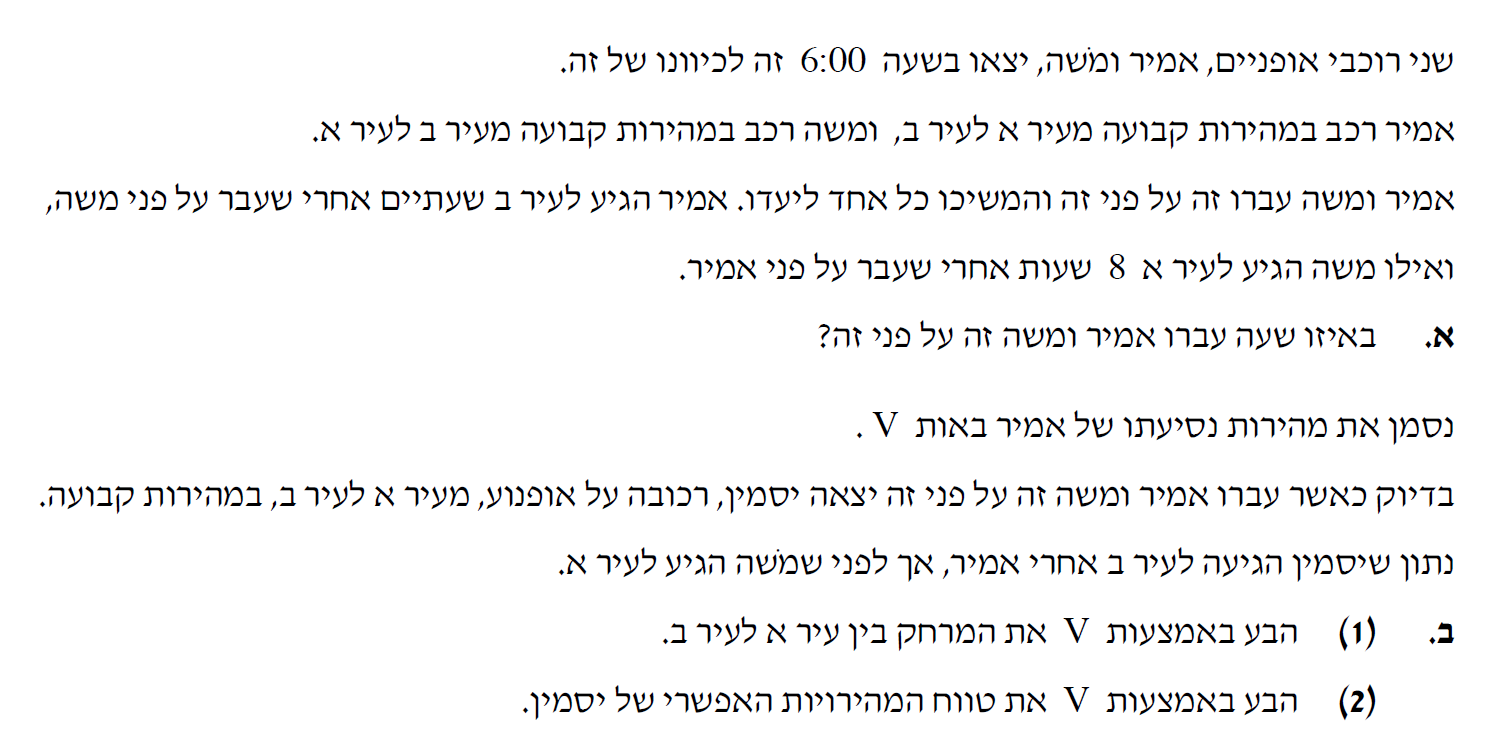
\includegraphics[width=\textwidth]{summer-2018a-1}
\end{center}

\begin{center}
\selectlanguage{english}
\begin{tikzpicture}[scale=.95]
\draw (0,0) node[left] {
\R{עיר א}
} node[below left,yshift=-6pt] {\p{06:00}} -- (10,0);
\draw (0,0) -- (0,6) node[left] {
\R{עיר ב}
};
\draw[dashed] (0,6) -- (10,6);
\draw[thick,name path=amir] (0,0) -- node[above left,near start] {
\R{אמיר}
} (6,6);
\draw[thick,name path=moshe] (0,6) -- node[above right,near start] {
\R{משה}
} (10,0);
\fill (0,6) circle [radius=2pt];
\fill (0,0) circle [radius=2pt];
\fill (6,6) circle [radius=2pt];
\fill (10,0) circle [radius=2pt];
\path[name intersections={of=amir and moshe,by=meeting}];
\fill (meeting) circle [radius=2pt];
\draw[dashed] (meeting) |- coordinate (meeting-time) (0,0);
\fill (meeting-time) circle [radius=2pt];
\draw[thick] (meeting-time) -- node[right,yshift=20pt,xshift=20pt] {
\R{יסמין}
} (8,6);
\fill (8,6) circle [radius=2pt];
\draw[dashed] (6,6) -- (6,0);
\draw[dashed] (8,6) -- (8,0);
\draw[dashed] (meeting) -| coordinate (meeting-distance) (0,0);
\fill (8,0) circle [radius=2pt];
\fill (meeting-distance) circle [radius=2pt];
\draw[<->] (0,-5mm) -- node[fill=white] {$t$} (meeting-time |- 0,-5mm);
\draw[<->] (meeting-time |- 0,-5mm) -- node[fill=white] {$2$} (6,-5mm);
\draw[<->] (meeting-time |- 0,-10mm) -- node[fill=white] {$8$} (10,-10mm);
\draw[<->] (meeting-time |- 0,-15mm) -- node[fill=white] {$t_y$} (8,-15mm);
\end{tikzpicture}
\end{center}

נסמן:
$=t$
הזמן עד למפגש בין אמיר למשה,
$=t_y$
זמן הנסיעה של יסמין מעיר א לעיר ב, 
$=v_y,v_m,v_a$
המהירויות של אמיר, משה ויסמין.


\textbf{סעיף א}

מהתרשים ניתן לראות לראות שיש
\textbf{שלושה}
ביטויים עבור המרחק בין הערים: )א( הרחק שנסע אמיר, )ב( המרחק שנסע משה, ו-)ג( סכום המרחקים שנסעו אמיר ומשה עד למפגש:
\[
tv_a + tv_m = (t+2) v_a = (t+8) v_m\,.
\]
משני הביטויים הראשונים אנו מקבלים:
\[
\frac{v_a}{v_m}=\frac{t}{2}\,.
\]

\np

נציב בשני הביטויים האחרונים:
\[
(t+2)\cdot \frac{tv_m}{2} = (t+8) v_m\,.
\]
$v_m$
מצטמצם ונקבל משוואה ריבועית
$t^2-16$
עם הפתרון החיובי 
$t=4$.

\textbf{שימו לב}

יש נטייה לעצור כאן כאשר חישבנו את הזמן 
$t$,
אבל עיון חוזר בשאלה מראה שהיא מבקשת את
\textbf{השעה}
של המפגש שהיא
\L{\p{10:00}}.

\smallskip

\textbf{סעיף ב}

המרחק בין הערים הוא 
$(t+2)v_a$.
חישבנו ש-%
$t=4$
ולכן המרחק הוא
$6v_a=6V$
)הסימון הנתון 
$V$
שונה מ-%
$v_a$
שבחרתי(.


\smallskip

\textbf{סעיף ג}

נתון שיסמין מגיע לעיר ב אחרי אמיר ולפני משה. מהתרשים רואים ש:
\[
2 < t_y < 8\,.
\]
זמן הוא מרחק חלקי מהירות ואת המרחק חישבנו בסעיף ב:
\[
2 < \frac{6V}{v_j} < 8\,.
\]
מכאן ש:
\[
\frac{3}{4}V < v_j < 3V\,
\]
כי כיווני האי-שוויון מתחלפים עם היפוך השבר.

%%%%%%%%%%%%%%%%%%%%%%%%%%%%%%%%%%%%%%%%%%%%%%%%%%%%%%%%%%%%%%%%

\np

\section{חורף תשע"ח}

\begin{center}
\selectlanguage{english}

\includegraphics[width=\textwidth]{winter-2018-1}
\end{center}

\begin{center}
\selectlanguage{english}
\begin{tikzpicture}[scale=1]
\draw (0,0) node[left] {$0$} -- (10,0);
\draw (0,0) -- (0,6);
\node at (-.5,1) {$\frac{1}{6}V_1$};
\node at (-.5,3) {$\frac{1}{2}V_1$};
\node at (-.5,6) {$V_1$};

\fill (0,0) circle [radius=2pt];
\draw[dashed] (0,1) -- (1,1);
\draw (0,0) -- node[below,xshift=4pt] {$4x$} (1,1);
\fill (1,1) circle [radius=2pt];

\draw[dashed] (0,3) -- (4,3);
\draw (1,1) -- node[below,xshift=4pt] {$3x$} (4,3);
\fill (4,3) circle [radius=2pt];

\draw[dashed] (0,6) -- (10,6);
\draw (4,3) -- node[below,xshift=4pt] {$x$} (10,6);
\fill (10,6) circle [radius=2pt];

\draw[dashed] (1,1) -- (1,0);
\draw[dashed] (4,3) -- (4,0);
\draw[dashed] (10,6) -- (10,0);

\draw[<->] (10.5,0) -- node[fill=white] {$V_2$} (10.5,5.5);

\fill (1,0) circle [radius=2pt];
\draw (1,0) -- node[below,xshift=4pt] {$x$} (4,1);
\fill (4,1) circle [radius=2pt];
\draw (4,1) -- node[below,xshift=4pt] {$3x$} (10,5.5);
\fill (10,5.5) circle [radius=2pt];

\draw[<->] (0,-.5) -- node[fill=white] {$t_1$} (1,-.5);
\draw[<->] (1,-.5) -- node[fill=white] {$t_2$} (4,-.5);
\draw[<->] (4,-.5) -- node[fill=white] {$t_3$} (10,-.5);


\end{tikzpicture}
\end{center}


נסמן:
$=x$
קצב המילוי של הצינורות )"אותו הספק"(,
$=t_1, t_2, t_3$
פרקי הזמן בין העברת הצינורות.

הקו העליון בתרשים מתאר את המילוי של בריכה א, והקו התחתון מתאר את מילוי של בריכה ב. שימו לב שככל שיותר צינורות ממלאים בריכה, השיפוע של הקו תלול יותר.

יש לנו שלוש קבונות של נעלמים: 
$x$,
שלושת ה-%
$t_i$
ושני ה-%
$V_i$.
אם נצליח להיפטר מ-%
$x$
או מה-%
$t_i$,
השני יצטמצם כאשר נחלק את ה-%
$V_i$.

נתחיל עם משוואות ההספק עבור בריכה א, כאשר בכל פרק זמן ממלאים את ההפרשים של הנפחים, למשל, בזמן 
$t_2$
בריכה א מתמלאת מששית מנפחה לחצי מנפחה:
\np
\erh{12pt}
\begin{equationarray*}{rcl}
4x t_1 &=& \frac{1}{6}V_1\\
3x t_2 &=& \left(\frac{1}{2}-\frac{1}{6}\right)V_1\\
xt_3&=&\left(1-\frac{1}{2}\right)V_1\,.
\end{equationarray*}
נשתמש במשוואת כדי לחשב את פרקי הזמן כתלות בנפח בבריכה:
\erh{12pt}
\begin{equationarray*}{rcl}
t_1 &=& \frac{V_1}{24x}\\
t_2 &=& \frac{V_1}{9x}\\
t_3&=&\frac{V_1}{2x}\,.
\end{equationarray*}
מהתרשים רואים שאפשר לבטא את הנפח של
$V_2$
כסכום: הנפח שמתמלא בפרק הזמן
$t_2$
ועוד הנפח המתמלא בפרק הזמן
$t_3$.
כאשר נציב את המשוואות שקבלנו עבור בפרקי הזמן, נקבל את הנפח של
$V_2$
כתלות ב-%
$V_1$
בלבד, כי המשתנה 
$x$ מצטמצם:
\erh{12pt}
\begin{equationarray*}{rcl}
V_2 &=& xt_2 + 3xt_3 = \frac{x V_1}{9x} + \frac{3x V_1}{2x}\ = \frac{29}{18}V_1\\
\frac{V_1}{V2} &=& \frac{18}{29}\,.
\end{equationarray*}
\textbf{הערה}

קיבלנו שהנפח של בריכה ב גדול מהנפח של בריכה א, עובדה שלא ידעתי כאשר ציירתי את התרשים עם נפח בריכה א גדול מנפח בריכה ב! אין לזה חשיבות. מטרת התרשים היא להציג את התסריט כדי שנוכל לכתוב את המשוואות הנכונות. 

פרט מעניין הוא שפרק הזמן הראשון
$t_1$
לא נחוץ לפתרון, כי המילוי של בריכה ב מתבצע בשני השלבים לאחר העברת הצינור הראשון.

%%%%%%%%%%%%%%%%%%%%%%%%%%%%%%%%%%%%%%%%%%%%%%%%%%%%%%%%%%%%%%%%

\np

\section{קיץ תשע"ז מועד ב}

\begin{center}
\selectlanguage{english}
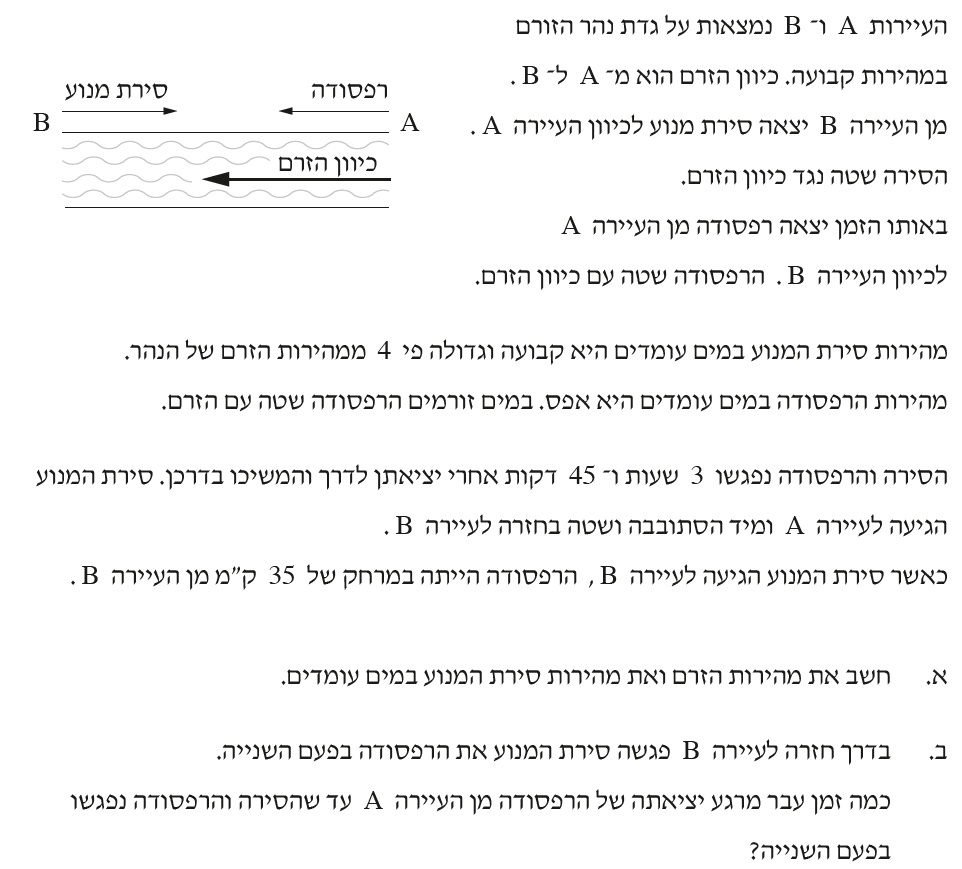
\includegraphics[width=.95\textwidth]{summer-2017b-1}
\end{center}

\vspace{-2ex}

\textbf{סעיף א}

\vspace{-3ex}

\begin{center}
\selectlanguage{english}
\begin{tikzpicture}[scale=.9]
\draw[name path=xaxis] (0,0) node[below left] {$A$} -- (10,0);
\draw (0,0) -- (0,6) node[above left] {$B$};
\draw[dashed] (0,6) -- (10,6);
\draw[thick,name path=raft] (0,0) -- node[left,near start,xshift=-4pt] {
\R{רפסודה}
} (10,4.5);
\draw[thick,name path=boat1] (0,6) -- node[right,near start,xshift=2pt] {
\R{סירה}
} (7,0);
\draw[thick,name path=boat2] (7,0) -- (10,6);
\path [name intersections={of=boat1 and raft,by=meeting1}];
\draw[dashed] (meeting1) |- coordinate (time) (0,0);
\draw[dashed] (meeting1) -| coordinate (distance) (0,0);
\draw[dashed] (10,0) -- (10,6);
\path[name path=t1] (7,0) -- (7,6);
\path [name intersections={of=raft and t1,by=a}];
\path [name intersections={of=raft and boat2,by=meeting2}];
\fill (meeting1) circle [radius=2pt];
\fill (meeting2) circle [radius=2pt];
\path [name path=t2] (meeting2) |- (0,0);
\path [name intersections={of=xaxis and t2,by=t2x}];
\fill (time) circle [radius=2pt];
\fill (0,0) circle [radius=2pt];
\fill (7,0) circle [radius=2pt];
\fill (10,6) circle [radius=2pt];
\fill (10,4.5) circle [radius=2pt];
\fill (0,6) circle [radius=2pt];
\fill (distance) circle [radius=2pt];
\draw[<->] (-.4,0) -- node[fill=white] {$d_r$} (distance -| -.4,0);
\draw[<->] (distance -| -.4,0) -- node[fill=white] {$d_s$} (-.4,6);
\draw[<->] (-.9,0) -- node[fill=white] {$d$} (-.9,6);
\draw[<->] (0,-.6) -- node[fill=white] { $15/4$} (time |- 0,-.6);
\draw[<->] (10.4,4.5) -- node[fill=white] { $35$} (10.4,6);
\end{tikzpicture}
\end{center}
נסמן:
$=d$
המרחק בין שני הנמלים,
$=d_r, d_s$
מרחקי ההפלגה של הסירה והרפסודה עד למפגש הראשון,
$=v_z$
מהירות הזרם,
$=v_s$
מהירות הסירה במים עומדים. ציר הזמן הוא בשעות.

\np

הזמן עד למפגש הראשון שווה עבור הסירה והרפסודה ויחס המהירויות של הסירה והזרם ידוע, כך שניתן לכתוב את משוואות התנועה עד למפגש. נתון:
\[
v_z = v_s/4\,.
\]
במפגש הראשון:
\[
d=d_s+d_r=\frac{15}{4}(v_s-v_z) + \frac{15}{4}v_z\,.
\]
מהירות הזרם מתאפסת ומתקבל:
\[
d = \frac{15}{4}v_s\,.
\]
כעת נכתוב משוואות תנועה כדי להשוות את הזמנים עד סוף הסיפור. בפרק הזמן שהסירה מפליגה ל-%
$A$
ובחזרה ל-%
$B$
)מרחק של
$d+d$(,
הרפסודה מפליגה מ-%
$A$
ומגיעה "כמעט" לנמל
$B$:
\[
\frac{d}{v_s-v_z} + \frac{d}{v_s+v_z} = \frac{d-35}{v_z}\,.
\]
מהנתון על יחס המהירויות ומחישוב המרחק, נציב עבור 
$v_z$
ו-%
$d$,
ונקבל משוואה עם נעלם אחד בלבד,
$v_s$.
הפתרון הוא
$v_s=20$
ומיחס המהירויות
$v_z=5$.
נחשב גם
$d=75$
שנצטרך בהמשך.

\smallskip

\textbf{סעיף ב}

נצייר תרשים חדש עם סימונים הקשורים למפגש השני.

\vspace{-1ex}

\begin{center}
\selectlanguage{english}
\begin{tikzpicture}[scale=.9]
\draw[name path=xaxis] (0,0) node[below left] {$A$} -- (10,0);
\draw (0,0) -- (0,6) node[above left] {$B$};
\draw[dashed] (0,6) -- (10,6);
\draw[thick,name path=raft] (0,0) -- node[left,near start,xshift=-4pt] {
\R{רפסודה}
} (10,4.5);
\draw[thick,name path=boat1] (0,6) -- node[right,near start,xshift=2pt] {
\R{סירה}
} (7,0);
\draw[thick,name path=boat2] (7,0) -- (10,6);
\path [name intersections={of=boat1 and raft,by=meeting1}];
\draw[dashed] (10,0) -- (10,6);
\path[name path=t1] (7,0) -- (7,6);
\path [name intersections={of=raft and t1,by=a}];
\path [name intersections={of=raft and boat2,by=meeting2}];
\fill (meeting2) circle [radius=2pt];
\fill (a) circle [radius=2pt];
\draw[<->] (7,.15) -- node[fill=white] {$d'$} (a);
\path [name path=t2] (meeting2) |- (0,0);
\fill (a -| meeting2) circle [radius=2pt];
\path [name intersections={of=xaxis and t2,by=t2x}];
\draw[<->] (a -| meeting2) -- node[fill=white,right,xshift=2pt] {$d''$} (meeting2);
\draw[dashed] (a -| meeting2) -- (t2x);
\draw[dashed] (a) -- (a -| meeting2) coordinate (one);
\fill (t2x) circle[radius=2pt];
\fill (0,0) circle [radius=2pt];
\fill (7,0) circle [radius=2pt];
\fill (10,6) circle [radius=2pt];
\fill (10,4.5) circle [radius=2pt];
\draw[<->] (0,-.4) -- node[fill=white] {$t_1$} (7,-.4);
\draw[<->] (7,-.4) -- node[fill=white] {$t_2$} (7,-.4 -| t2x);
\end{tikzpicture}
\end{center}

\vspace{-1ex}


נסמן:
$=t_1$
הזמן שהסירה מפליגה ל-%
$A$
ל-%
$B$,
$=t_2$
הזמן שהסירה מפליגה מ-%
$A$
למפגש השני,
$=d'$
המרחק שהרפסודה מפליגה בזמן
$t_1$,
$=d''$
המרחק שהרפסודה מפליגה בזמן
$t_2$.

\smallskip
קל לחשב
$t_1$
ממשוואת התנועה של הסירה:
\[
t_1=\frac{d}{v_s-v_z}=\frac{75}{20-5}=5\,,
\]

ולחשב את המרחק
$d'$
מהמשוואה של הרפסודה:
\[
d'=v_zt_1=5\cdot 5=25\,.
\]

\np

נשאר לחשב את פרק הזמן
$t_2$.
בפרק זמן זה הסירה מפליגה מרחק
$d'+d''$
והרפסודה מפליגה מרחק
$d''$.
המהירויות ידועות, כך שיש לנו שתי משוואות עבור
$t_2$:
\erh{14pt}
\begin{equationarray*}{rcl}
t_2&=&\frac{d'+d''}{v_s+v_z} = 
\frac{25+d''}{25}\\
t_2&=&\frac{d''}{v_z}=\frac{d''}{5}\,.
\end{equationarray*}
נפתור את המשוואה ונקבל:
\erh{14pt}
\begin{equationarray*}{rcl}
d''&=&\frac{25}{4}\\
t_2&=&\frac{d''}{v_z}=\frac{5}{4}\,.
\end{equationarray*}
\textbf{שימו לב}

שהשאלה מבקשת את זמן ההפלגה של הרפסודה מנמל
$A$
ועד למפגש השני:
\[
t_1+t_2=5+\frac{5}{4}=\frac{25}{4}\,.
\]


%%%%%%%%%%%%%%%%%%%%%%%%%%%%%%%%%%%%%%%%%%%%%%%%%%%%%%%%%%%%%%%%

\np

\section{קיץ תשע"ז מועד א}

\begin{center}
\selectlanguage{english}
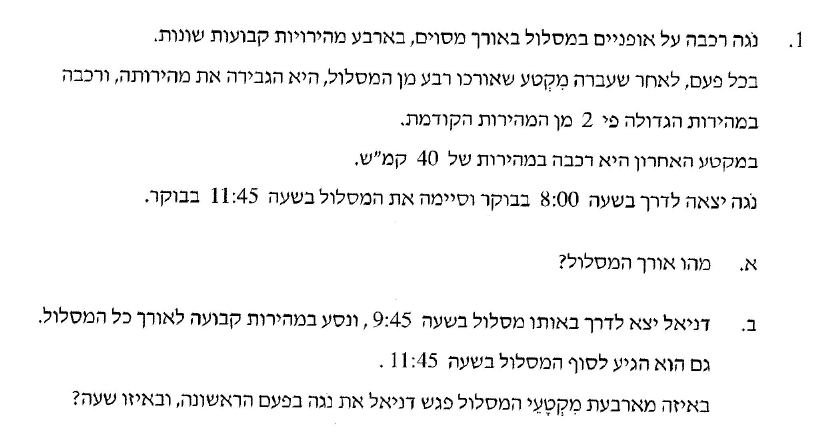
\includegraphics[width=\textwidth]{summer-2017a-1}
\end{center}

\begin{center}
\selectlanguage{english}
\begin{tikzpicture}[scale=1]
\draw (0,0) node[below] {\p{08:00}} -- (11.25,0) node[below] {\p{11:45}};
\draw (0,0) -- (0,6);
\draw[thick,name path=noga] (0,0) -- (6,1.5) -- (9,3) -- (10.5,4.5) --  node[right] {
\R{נגה}
} (11.25,6);
\draw[dashed] (0,6) -- +(11.25,0);
\draw[dashed] (0,4.5) -- +(10.5,0);
\draw[dashed] (0,3) -- +(9,0);
\draw[dashed] (0,1.5) -- +(6,0);
\draw[dashed] (6,0) -- (6,1.5);
\draw[dashed] (9,0) -- (9,3);
\draw[dashed] (10.5,0) -- (10.5,4.5);
\draw[dashed] (11.25,0) -- (11.25,6);
\fill (0,0) circle [radius=2pt];
\fill (6,1.5) circle [radius=2pt];
\fill (9,3) circle [radius=2pt];
\fill (10.5,4.5) circle [radius=2pt];
\fill (11.25,6) circle [radius=2pt];
\path (0,0) -- node[left] {$x$} (0,1.5) -- node[left] {$x$} (0,3) -- node[left] {$x$} (0,4.5) -- node[left] {$x$} (0,6);
\draw[thick,name path=dan] (5.25,0) node[below] {\p{09:45}} --  node[left,xshift=16pt,yshift=20pt] {
\R{דניאל}
} (11.25,6);
\path [name intersections={of=noga and dan,by=meeting}];
\draw[dashed] (meeting) |- coordinate (time) (0,0);
\fill (5.25,0) circle [radius=2pt];
\fill (meeting) circle [radius=2pt];
\fill (time) circle [radius=2pt];
\draw[<->] (0,-7mm) -- node[below] {$t_1$} +(6,0);
\draw[<->] (6,-7mm) -- node[below] {$t_2$} +(3,0);
\draw[<->] (6,3mm) -- node[above] {$t$} (time |- 6,3mm);
\draw[<->] (9,-7mm) -- node[below] {$t_3$} +(1.5,0);
\draw[<->] (10.5,-7mm) -- node[below] {$t_4$} +(.75,0);
\end{tikzpicture}
\end{center}

נסמן:
$=x$
המרחק של מקטע,
$=t_1,t_2,t_3,t_4$
זמני רכיבה של נגה במקטעים.

נתון: 
$=40$
המהירות במקטע האחרון, לכן המהירויות של המקטעים האחרים הן
$5,10,20$.

\textbf{סעיף א}

נתון לנו הזמן הכולל והמהירויות )אמנם רק המהירות האחרונה נתונה, אבל אפשר לחשב את האחרות(, והנעלם היחיד הוא המרחק. נסכם את הזמנים של המקטעים:
\[
\left(\frac{x}{5}+\frac{x}{10}+\frac{x}{20}+\frac{x}{40}\right) = \frac{15}{4}\,.
\]
הפתרון הוא
$x=10$
ולכן אורך המסלול הוא
$40$
ק"מ.

\np

\textbf{סעיף ב}

חישבנו את המרחק ונתון הזמן של דניאל. המהירות של דניאל היא 
$40/2=20$
קמ"ש.

אפשר אולי למצוא נוסחה עבור המפגש, אבל פשוט יותר לעבור מקטע מקטע ולבדוק אם המפגש מתקיים באותו מקטע.

נגה עוברת
$10$
ק"מ בכל מקטע. מה המרחק שעובר דניאל עד סוף המקטע הראשון?

$t_1 = 10/5 = 2$
כך שסוף המקטע הוא ב- 
\L{\p{10:00}}.
דניאל רוכב רבע שעה מ-
\L{\p{09:45}}
ועד
\L{\p{10:00}}
ולכן המרחק שהוא עובר הוא רק
$\displaystyle 20\cdot\frac{1}{4} = 5$
ק"מ והמפגש לא התקיים במקטע הראשון.


מתי נגה מגיעה לסוף המקטע השני?
$t_2=10/10 =1$
כך שסוף המקטע הוא ב-%
\L{\p{11:00}}.
בשעה ורבע בין 
\L{\p{09:45}}
ל
\L{\p{11:00}}
דניאל רוכב
$\displaystyle 20\cdot \frac{5}{4}=25$
ק"מ, מרחק גדול מהמרחק של נגה, לכן המפגש מתקיים במקטע השני.

\medskip

נשאר רק לחשב את פרק הזמן בתוך המקטע השני עד למפגש, שנסמן
$t$.
נכתוב משוואה למרחקים השווים של נגה ודניאל. נגה רכבה
$10$
ק"מ עד סוף הקטע הראשון ודניאל רכב 
$5$
ק"מ. מסוף הקטע הראשון, הם רכבו 
$t$
שעות, כל אחד במהירות שלו:
\erh{12pt}
\begin{equationarray*}{rcl}
10 + 10t &=& 5 + 20t\\
t&=&\frac{1}{2}\,.
\end{equationarray*}
\textbf{שימו לב}

השאלה מבקשת את שעת המפגש. כבר חישבנו שתחילת המקטע השני בשעה
\L{\p{10:00}},
ולכן שעת המפגש היא
\L{\p{10:30}}.

%%%%%%%%%%%%%%%%%%%%%%%%%%%%%%%%%%%%%%%%%%%%%%%%%%%%%%%%%%%%%%%%

\np

\section{חורף תשע"ז}

\begin{center}
\selectlanguage{english}
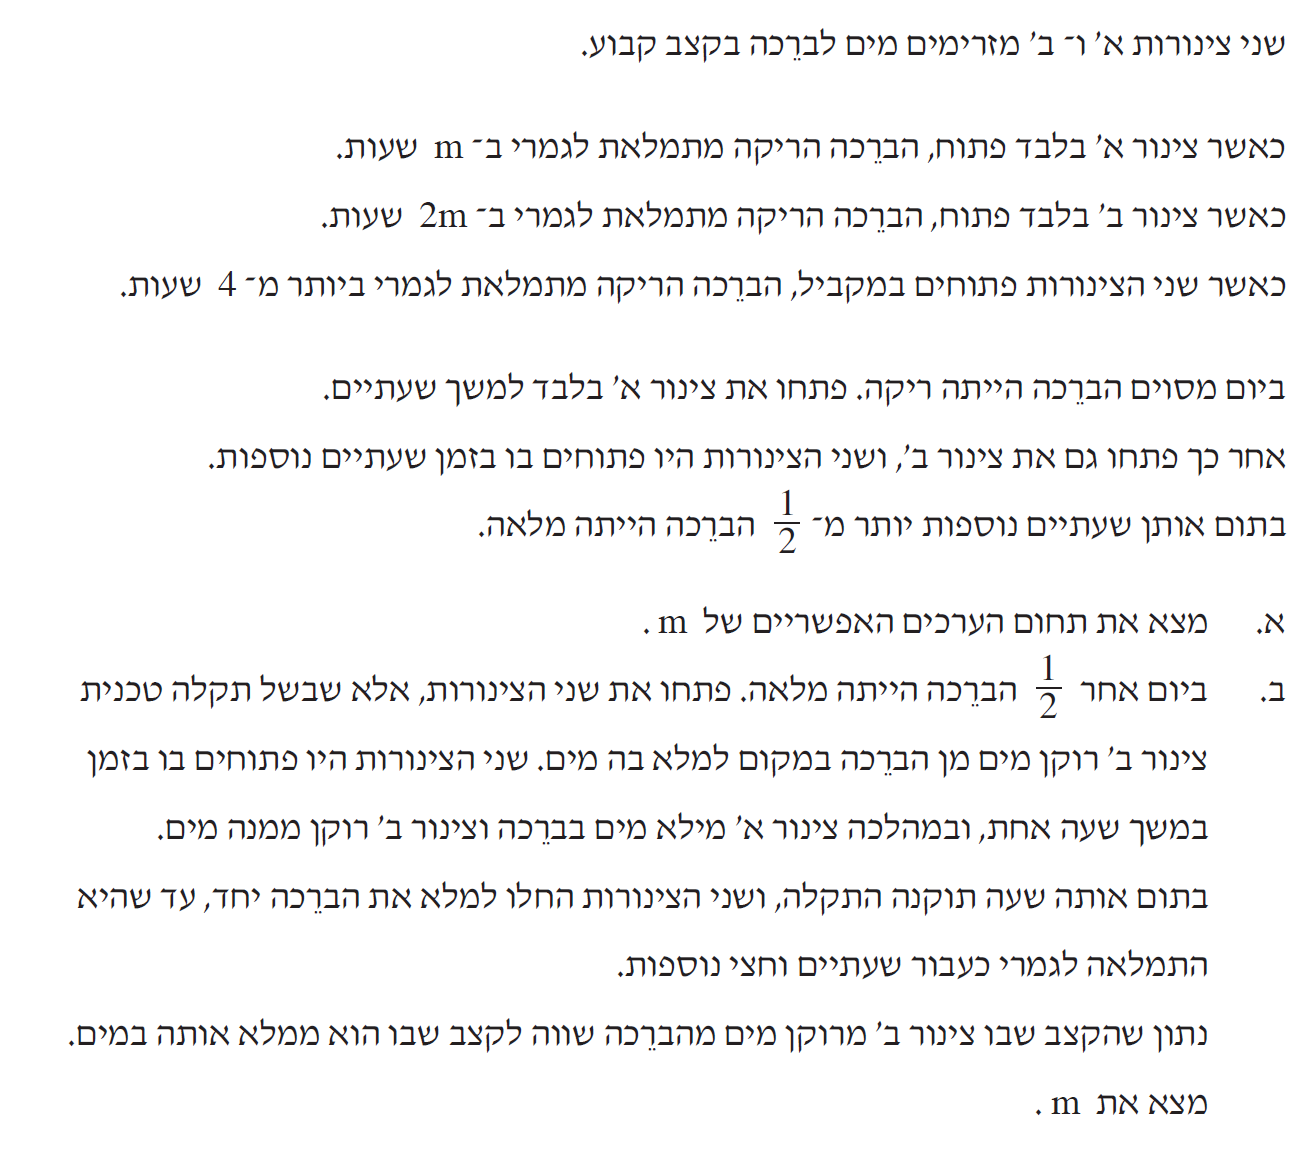
\includegraphics[width=.9\textwidth]{winter-2017-1}
\end{center}

%\vspace{-3ex}

\textbf{סעיף א}

\begin{center}
\selectlanguage{english}
\begin{tikzpicture}[scale=.8]
\draw (0,0) -- (10,0);
\draw (0,0) node[left] {\R{בריכה ריקה}} -- (0,6) node[left] {\R{בריכה מליאה}};
\draw[dashed] (0,6) -- (10,6);
\draw[thick] (0,0) -- node[right,near end,xshift=2mm,yshift=-2mm] {
\R{ב}
} node[right,xshift=12mm,yshift=4mm] {$\displaystyle\frac{1}{2m}$}(9,6);
\draw[thick] (0,0) -- node[left,near end,xshift=-3mm] {
\R{א}
} node[left,xshift=-2mm,yshift=3mm] {$\displaystyle\frac{1}{m}$} (4.5,6);
\draw[dashed] (9,6) -- (9,0);
\draw[dashed] (4.5,6) -- (4.5,0);
\draw[<->] (0,-.6) -- node[fill=white] {$m$} (4.5,-.6);
\draw[<->] (0,-1.2) -- node[fill=white] {$2m$} (9,-1.2);
\end{tikzpicture}
\end{center}

%\vspace{-2ex}

כאשר שני הצינורות פתוחים, ההספק הכולל הוא סכום ההספקים של הצינורות. לפי הנתונים:
\[
1/\left(\frac{1}{m}+\frac{1}{2m}\right) > 4\,,
\]
כך ש-%
$m>6$.

\np

\begin{center}
\selectlanguage{english}
\begin{tikzpicture}
\draw (0,0) -- (10,0);
\draw (0,0) node[left] {\R{בריכה ריקה}}
-- (0,4) node[left] {\R{בריכה מליאה}};
\draw[thick] (4,0) -- node[above,near end,yshift=2mm] {
\R{ב}
} node[above,near start,yshift=2mm] {$\displaystyle\frac{1}{2m}$}(8,1);
\draw[thick] (0,0) -- node[left,near end,xshift=-3mm] {
\R{א}
} node[left,xshift=-2mm,yshift=3mm] {$\displaystyle\frac{1}{m}$} (8,4);
\draw[dashed] (8,4) -- (8,0);
\draw[dashed] (4,2) -- (4,0);
\draw[<->] (0,-.6) -- node[fill=white] {$2$} (4,-.6);
\draw[<->] (0,-1.2) -- node[fill=white] {$4$} (8,-1.2);
\draw[<->] (9,0) -- node[fill=white] {$w_a$} (9,4);
\draw[<->] (8.5,0) -- node[fill=white] {$w_b$} (8.5,1);
\end{tikzpicture}
\end{center}
נסמן:
$=w_a$
כמות המים שמילא צינור א,
$=w_b$
כמות המים שמילא צינור ב.

\smallskip

כמות המים לאחר ארבע שעות שווה לסכום הכמויות שכל צינור מילא והיא לפחות מחצית הבריכה:
\[
w_a + w_b = \frac{1}{m}\cdot 4 + \frac{1}{2m}\cdot 2 > \frac{1}{2}\,.
\]
מכאן,
$m<10$.

\smallskip

\textbf{סעיף ב}

\begin{center}
\selectlanguage{english}
\begin{tikzpicture}[scale=.9]
\draw (0,0) -- (9,0);
\draw (0,0) node[left] {\R{בריכה ריקה}}
-- (0,6) node[left] {\R{בריכה מליאה}};
\draw[dashed] (0,6) -- (9,6);
\draw[thick] (0,3) -- node[below right,xshift=10mm,yshift=-4mm] {$\displaystyle\frac{1}{m}-\frac{1}{2m}=\frac{1}{2m}$} (2,3.5);
\draw[->] (2.2,2.15) -- +(140:1.6cm);
\draw[thick] (2,3.5) -- node[left,xshift=-4mm,yshift=3mm] {$\displaystyle\frac{1}{m}+\frac{1}{2m}=\frac{3}{2m}$} (7,6);
\draw[dashed] (2,3.5) -- (2,0);
\draw[dashed] (2,3.5) -- (0,3.5);
\draw[dashed] (7,6) -- (7,0);
\draw[<->] (0,-.6) -- node[fill=white] {$1$} (2,-.6);
\draw[<->] (2,-1.2) -- node[fill=white] {$2.5$} (7,-1.2);
\node at (-.4,3) {$\displaystyle\frac{1}{2}$};
\end{tikzpicture}
\end{center}
כדי למלא את הבריכה, מתחילים ממחצית הכמות, מוסיפים )מחסירים כי שלילי( את הכמות של השעה הראשונה, ומוסיפים את הכמות מפרק הזמן השני של שעתיים וחצי:
\[
\frac{1}{2} + \left(\frac{1}{m}-\frac{1}{2m}\right)\cdot 1 + \left(\frac{1}{m}+\frac{1}{2m}\right)\cdot 2.5 = 1\,.
\]
הפתרון הוא
$m=8.5$.

%%%%%%%%%%%%%%%%%%%%%%%%%%%%%%%%%%%%%%%%%%%%%%%%%%%%%%%%%%%%%%%%

\np

\section{קיץ תשע"ו, מועד ב}

\begin{center}
\selectlanguage{english}
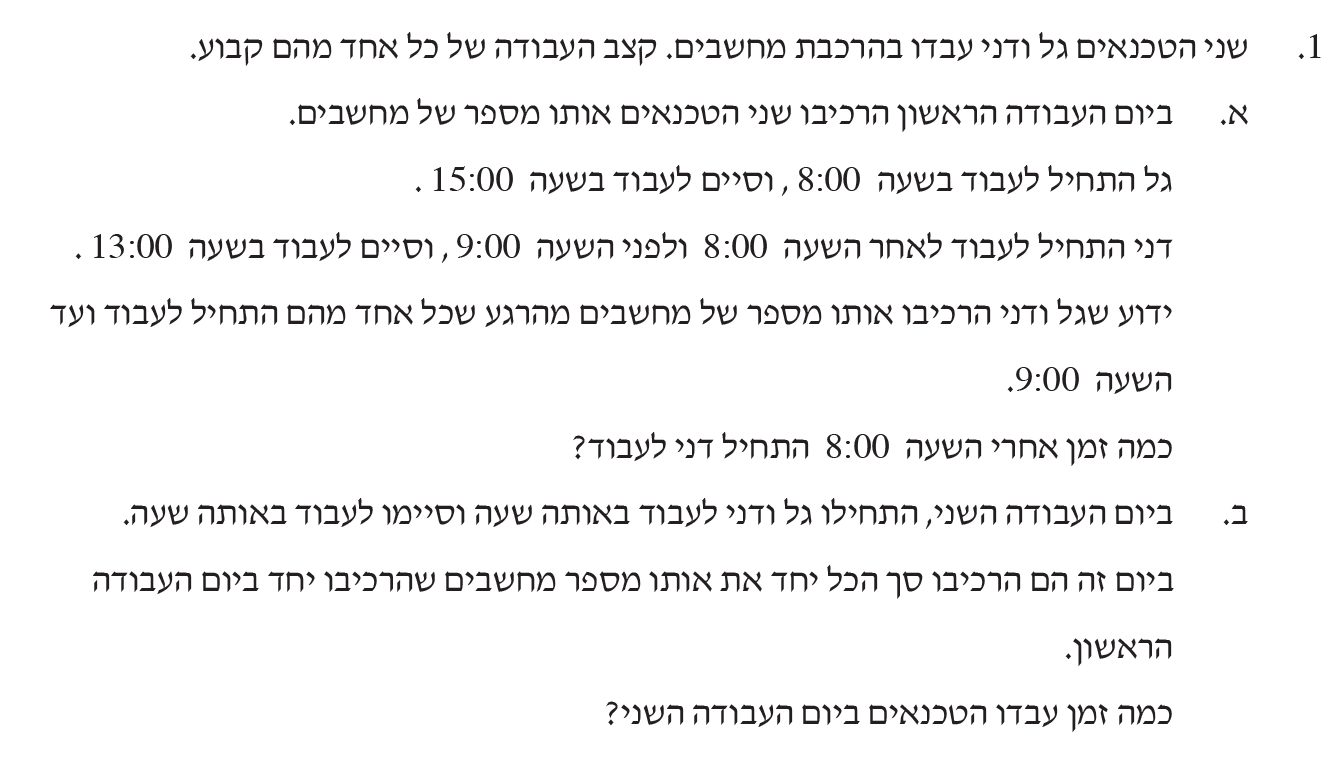
\includegraphics[width=\textwidth]{summer-2016b-1}
\end{center}

\textbf{סעיף א}

\begin{center}
\selectlanguage{english}
\begin{tikzpicture}
\draw (0,0) -- (10,0);
\draw (0,0) node[above left] {\R{אף מחשב לא הורכב}}
-- (0,6) node[left] {\R{כל המחשבים הורכבו}};
\draw[dashed] (0,6) -- (10,6);
\draw[thick,name path=gal] (0,0) -- node[right,near end,xshift=3mm] {
\R{גל}
} node[right,xshift=7mm] {$\displaystyle\frac{1}{7}$}(10,6);
\draw[thick,name path=danny] (1.2,0) -- node[left,near end,xshift=-3mm] {
\R{דני}
} node[left,yshift=3mm] {$\displaystyle\frac{1}{(1-t)+4}$} (7,6);
\draw[dashed] (7,6) -- (7,0);
\draw[dashed] (10,6) -- (10,0);
\path [name intersections={of=gal and danny,by=inter}];
\fill (inter) circle [radius=2pt];
\draw[dashed] (inter) -- (inter |- 0,0);
\draw[dashed] (inter) -- (inter -| 0,0);
\node[below] at (0,0) {\p{08:00}};
\node[below] at (1.2,0) {$t$};
\node[below] at (inter |- 0,0) {\p{09:00}};
\node[below] at (7,0) {\p{13:00}};
\node[below] at (10,0) {\p{15:00}};
\end{tikzpicture}
\end{center}

נסמן:
$=t$
הזמן שדני התחיל בהרכבה.

נשתמש בנתונים כדי למצוא ביטויים עבור ההספקים של דני וגל. נתייחס לסך המחשבים שהרכיב כל אחד כיחידת עבודה אחת. גל עבד שבע שעות ולכן ההספק שלו הוא
$\displaystyle \frac{1}{7}$,
ודני עבד 
$1-t$
עד לשעה 
\L{\p{09:00}}
ואחר כך עוד ארבע שעות. ההספק שלו הוא
$\displaystyle \frac{1}{(1-t)+4}$.

\np
נתון שבשעה 
\L{\p{09:00}}
שניהם סיימו להרכיב אותו כמות של מחשבים:
\[
\frac{1}{7}\cdot 1 = \frac{1}{(1-t)+4} \cdot (1-t)\,,
\]
ולכן דני התחיל לעבוד
$\displaystyle t=\frac{1}{3}$
שעה לאחר
\L{\p{08:00}}.

\smallskip

\textbf{סעיף ב}

נצייר תרשים חדש עם המידע הרלוונטי לסעיף זה.

\begin{center}
\selectlanguage{english}
\begin{tikzpicture}
\draw (0,0) -- (10,0);
\draw (0,0) node[above left] {\R{אף מחשב לא הורכב}}
-- (0,6) node[left] {\R{כל המחשבים הורכבו}};
\draw[dashed] (0,6) -- (10,6);
\draw[thick] (0,0) -- node[right,near end,xshift=2mm,yshift=-2mm] {
\R{גל}
} node[right,xshift=6mm,yshift=-3mm] {$\displaystyle\frac{1}{7}$}(8,2.5);
\draw[thick] (0,0) -- node[left,near end,xshift=-3mm] {
\R{דני}
} node[left,xshift=-2mm,yshift=3mm] {$\displaystyle\frac{3}{14}$} (8,6);
\draw[dashed] (8,6) -- (8,0);
\draw[<->] (0,-.6) -- node[fill=white] {$T$} (8,-.6);
\draw[<->] (8.6,0) -- node[fill=white] {$w_g$} (8.6,2.5);
\draw[<->] (9.2,0) -- node[fill=white] {$w_d$} (9.2,6);
\end{tikzpicture}
\end{center}
נסמן: 
$=T$
הזמן ששניהם עבדו ביום השני. על התרשים סימנו גם את כמות העבודה שעשה כל אחד מהם:
$=w_g$
העבודה של גל,
$=w_d$
העבודה של דני.

\smallskip

בסעיף א הערנו שההספק של גל הוא
$\displaystyle \frac{1}{7}$,
וחישבנו שדני עבד:
\[
\left(1-\frac{1}{3}\right)+4=\frac{14}{3}
\]
שעות. ההספק שלו הוא:
\[
\frac{1}{\frac{14}{3}}=\frac{3}{14}\,.
\]
נתון שהם סיימו אותה כמות עבודה כמו היום הראשון:
\[
1+1=w_g+w_d=\frac{1}{7}T + \frac{3}{14}T\,,
\]
והפתרון הוא 
$T=\displaystyle \frac{28}{5}$.

%%%%%%%%%%%%%%%%%%%%%%%%%%%%%%%%%%%%%%%%%%%%%%%%%%%%%%%%%%%%%%%%

\np

\section{קיץ תשע"ו מועד א}

\begin{center}
\selectlanguage{english}
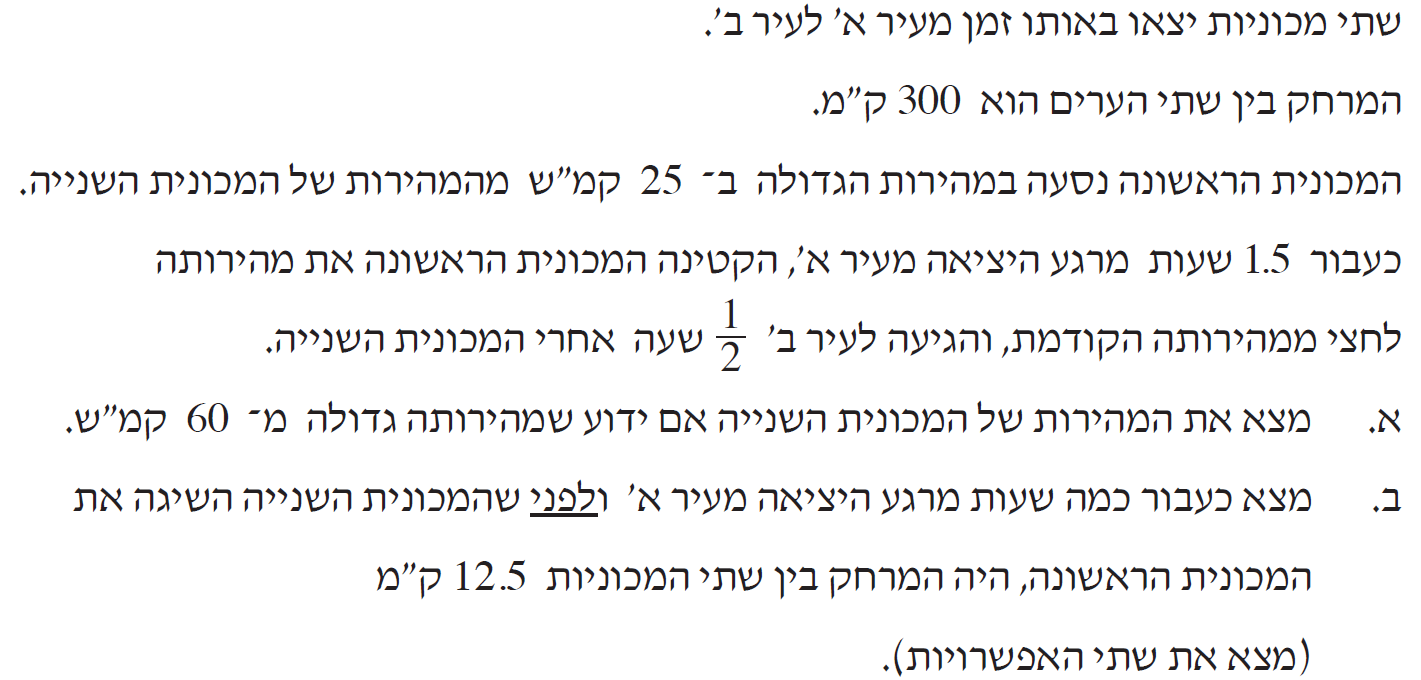
\includegraphics[width=.9\textwidth]{summer-2016a-1}
\end{center}

\begin{center}
\selectlanguage{english}
\begin{tikzpicture}
\draw (0,0) node[left] {
\R{א}
} -- (10,0);
\draw (0,0) -- node[left] {
\R{ק"מ}
$300$} (0,6) node[left] {
\R{ב}
};
\draw[dashed] (0,6) -- (10,6);
\draw[thick,name path=car1] (0,0) -- (3,4) coordinate (change) -- node[above left,near start] {$1$
\R{מכונית}
} (10,6);
\draw[thick,name path=car2] (0,0) -- node[right,xshift=1pt,yshift=-12pt] {$2$
\R{מכונית}
} (7,6);
\draw[dashed] (change) |- coordinate (time) (0,0);
\draw[dashed] (7,6) -- (7,0);
\draw[dashed] (10,6) -- (10,0);
\fill (0,0) circle [radius=2pt];
\fill (7,0) circle [radius=2pt];
\fill (10,0) circle [radius=2pt];
\fill (change) circle [radius=2pt];
\fill (time) circle [radius=2pt];
\draw[<->] (0,-5mm) -- node[fill=white] {
\R{שעות}
$3/2$} (time |- 0,-5mm);
\draw[<->] (7,-5mm) -- node[fill=white] {
\R{שעה}
$1/2$} (10,-5mm);
\draw[<->] (0,-10mm) -- node[fill=white] {$t$} (7,-10mm);
\end{tikzpicture}
\end{center}


נסמן:
$=v_1$
מהירות התחלתית של מכונית
$1$,
$=v_2$
מהירות של מכונית
$2$,
$=t$
זמן נסיעה של מכונית
$2$
מעיר א' עד לעיר ב'.

נתון:
$v_1 = v_2+25$.
השיפוע של הקו של מכונית 
$1$
גדולה מהשיפוע של הקו של מכונית 
$2$.

\textbf{סעיף א}

שתי המכוניות נסעו אותו מרחק מעיר א לעיר ב. נכתוב את משוואות התנועה של שתי המכוניות:
\begin{eqnarray*}
v_1\cdot\frac{3}{2} + \frac{v_1}{2}\left(\left(t-\frac{3}{2}\right)+\frac{1}{2}\right) &=& 300\\
v_2t &=& 300\,.
\end{eqnarray*}
נציב 
$v_1 = v_2+25$,
$t = 300/v_2$
במשוואה הראשונה ונקבל משוואה ריבועית ב-%
$v_2$:
\[
v_2^2 - 125v_2 + 3750 = 0\,.
\]
השורשים הם
$50,75$
ונתון ש-%
$v_2>60$
כך שיש לבחור
$v_2=75$
קמ"ש.

\np

\textbf{סעיף ב}

נצייר תרשים חדש עם המידע הרלוונטי עבור סעיף זה.

\begin{center}
\selectlanguage{english}
\begin{tikzpicture}
\draw (0,0) node[left] {
\R{א}
} -- (10,0);
\draw (0,0) -- node[left] {
\R{ק"מ}
$300$} (0,6) node[left] {
\R{ב}
};
\draw[dashed] (0,6) -- (10,6);
\draw[thick,name path=car1] (0,0) -- (3,4) coordinate (change) -- node[above left,near start] {$1$
\R{מכונית}
} (10,6);
\draw[thick,name path=car2] (0,0) -- node[right,xshift=32pt,yshift=20pt] {$2$
\R{מכונית}
} (8,6);
\path [name path=time1] (1.2,0) -- (1.2,6);
\path [name path=time2] (5,0) -- (5,6);
\path [name intersections={of=car1 and time1,by=meeting11}];
\path [name intersections={of=car1 and time2,by=meeting12}];
\path [name intersections={of=car2 and time1,by=meeting21}];
\path [name intersections={of=car2 and time2,by=meeting22}];
\draw[thick] (meeting11) -- (meeting21);
\draw[thick] (meeting12) -- (meeting22);
\draw[dashed] (meeting21) |- coordinate (t1) (0,0);
\draw[dashed] (meeting22) |- coordinate (t2) (0,0);
\draw[dashed] (change) |- coordinate (time) (0,0);
\fill (0,0) circle [radius=2pt];
\fill (t1) circle [radius=2pt];
\fill (t2) circle [radius=2pt];
\fill (change) circle [radius=2pt];
\fill (time) circle [radius=2pt];
\draw[<->] (0,-5mm) -- node[fill=white] {$t_1$} (t1 |- 0,-5mm);
\draw[<->] (0,-10mm) -- node[fill=white] {
\R{שעות}
$3/2$} (time |- 0,-10mm);
\draw[<->] (0,-15mm) -- node[fill=white] {$t_2$} (t2 |- 0,-15mm);
\end{tikzpicture}
\end{center}

הקווים האנכיים הכלואים בין הקווים של שתי המכוניות מסמנים מרחק של
$12.5$
ק"מ. קו אחד הוא לפני שינוי המהירות בזמן
$t_1$
מתחילת הנסיעה וקו שני לאחר שינוי המהירות.

בסעיף א' חישבנו
$v_2=75$
ולכן
$v_1=v_2+25=100$.

\smallskip

נכתוב את המשוואות עבור הפרשי המרחקים:
\begin{eqnarray*}
100t_1 - 75t_1 &=& 12.5\\
\left(100\cdot \frac{3}{2} + 50\left(t_2-\frac{3}{2}\right)\right) - 75t_2&=& 12.5\,.
\end{eqnarray*}
הפתרונות הם
$\displaystyle t=\frac{1}{2}, t_2=\frac{5}{2}$
שעות.


%%%%%%%%%%%%%%%%%%%%%%%%%%%%%%%%%%%%%%%%%%%%%%%%%%%%%%%%%%%%%%%%

\np

\section{חורף תשע"ו}

\begin{center}
\selectlanguage{english}
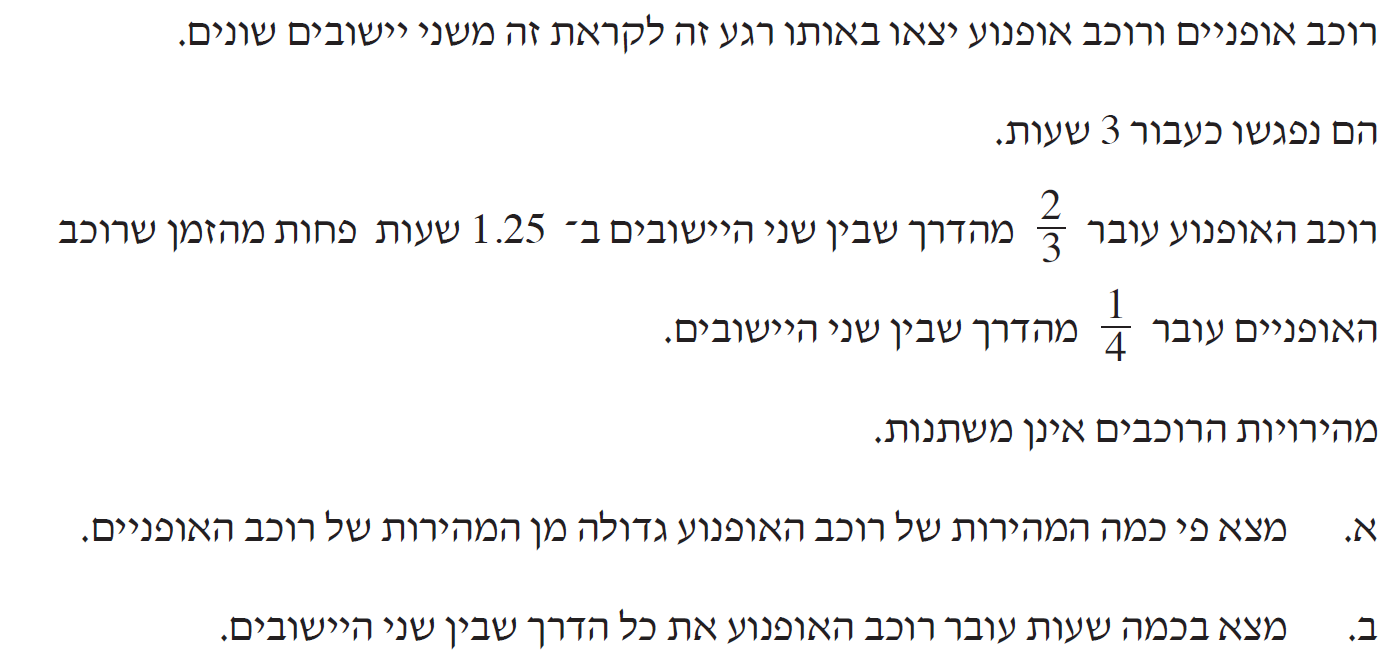
\includegraphics[width=.9\textwidth]{winter-2016-1}
\end{center}

\textbf{סעיף א}

\begin{center}
\selectlanguage{english}
\begin{tikzpicture}
\draw (0,0) node[left] {$A$} -- (10,0);
\draw (0,0) -- (0,6) node[left] {$B$};
\draw[dashed] (0,6) -- (10,6);
\draw[thick,name path=motor] (0,0) -- node[right,near start,xshift=1pt,yshift=-4pt] {
\R{אופנוע}
} (4,6);
\draw[thick,name path=bike] (0,6) -- node[above,near end,xshift=44pt,yshift=-10pt] {
\R{אופניים}
} (8,4);
\node at (8.4,3.7) {$\cdots$};
\path [name intersections={of=motor and bike,by=meeting}];
\coordinate (fourth) at (0,4.5);
\coordinate (two-thirds) at (0,3.5);
\path [name path=path-fourth] (fourth) -- +(6,0);
\path [name path=path-two-thirds] (two-thirds) -- +(6,0);
\path [name intersections={of=path-fourth and bike,by=meeting-fourth}];
\path [name intersections={of=path-two-thirds and motor,by=meeting-two-thirds}];
\draw[dashed] (meeting) |- coordinate (time) (0,0);
\draw[dashed] (meeting-fourth) -| coordinate (fourth-y) (0,0);
\draw[dashed] (meeting-fourth) |- coordinate (fourth-x) (0,0);
\draw[dashed] (meeting-two-thirds) -| coordinate (two-thirds-y) (0,0);
\draw[dashed] (meeting-two-thirds) |- coordinate (two-thirds-x) (0,0);
\fill (meeting) circle [radius=2pt];
\fill (time) circle [radius=2pt];
\fill (0,0) circle [radius=2pt];
\fill (two-thirds) circle [radius=2pt];
\fill (fourth) circle [radius=2pt];
\fill (fourth-x) circle [radius=2pt];
\fill (fourth-y) circle [radius=2pt];
\fill (meeting-fourth) circle [radius=2pt];
\fill (two-thirds-x) circle [radius=2pt];
\fill (two-thirds-y) circle [radius=2pt];
\fill (meeting-two-thirds) circle [radius=2pt];
\path (0,0) -- node[left] {$\frac{2}{3}x$} (two-thirds-y);
\path (0,6) -- node[left] {$\frac{1}{4}x$} (fourth-y);
\draw[<->] (0,-.5) -- node[fill=white] {$3$} (time |- 0,-.5);
\draw[<->] (fourth-x |- 0,-1) -- node[fill=white] {$5/4$} (two-thirds-x |- 0,-1);
\draw[<->] (0,-1.5) -- node[fill=white] {$T_m$} (two-thirds-x |- 0,-1.5);
\draw[<->] (0,-2) -- node[fill=white] {$T_b$} (fourth-x |- 0,-2);
\end{tikzpicture}
\end{center}

נסמן:
$=v_b$
מהירות אופניים,
$=v_m$
מהירות אופנוע,
$=x$
מרחק בין הערים,
$=T_m$
פרק הזמן שהאופנוע עובר
$\frac{2}{3}$
מהמרחק,
$=T_b$
פרק הזמן שהאופניים עובר
$\frac{1}{4}$
מהמרחק.

כאשר שני כלי הרכב נפגשים סכום המרחקים שהם עברו הוא המרחק בין הנקודות. המרחק לא נתון ולכן אנו משתמשים בנעלם
$x$:
\[
x = 3v_b + 3 v_m\,.
\]
הנתון השני הוא הקשר בין זמני הנסיעה של חלקי המרחק בין היישובים
$T_b=T_m+1.25$:
\[
\frac{x/4}{v_b} = \frac{2x/3}{v_m} + \frac{5}{4}\,.
\]
\np

נציב עבור
$x$,
נסמן את היחס בין המהירויות
$r=\disfrac{v_m}{v_b}$
ונקבל משוואה הריבועית:
\erh{14pt}
\begin{equationarray*}{rcl}
\frac{3v_b+3v_m}{4v_b}&=&\frac{2(3v_b+3v_m)}{3v_m}+\frac{5}{4}\\
\frac{3}{4}+\frac{3}{4}r&=&\frac{2}{r}+2+\frac{5}{4}\\
3r^2 - 10r - 8 &=& 0\,.
\end{equationarray*}
השורש החיובי הוא
$r=\disfrac{v_m}{v_b}=4$.


\textbf{סעיף ב}

נתונה משוואת המרחק בין היישובים:
\[
x = 3v_b + 3 v_m\,.
\]
נשתמש ביחס שחישבנו בסעיף א כדי לחשב את הזמן של נסיעת האופנוע:
\[
\frac{x}{v_m} = \frac{3v_b + 3 v_m}{v_m}=3\frac{v_b}{v_m}+3=\frac{3}{r}+3=\frac{3}{4}+3=\frac{15}{4}\quad \textrm{\R{שעות}}\,.
\]

%%%%%%%%%%%%%%%%%%%%%%%%%%%%%%%%%%%%%%%%%%%%%%%%%%%%%%%%%%%%%%%%

\np

\section{קיץ תשע"ה מועד ב}

\begin{center}
\selectlanguage{english}
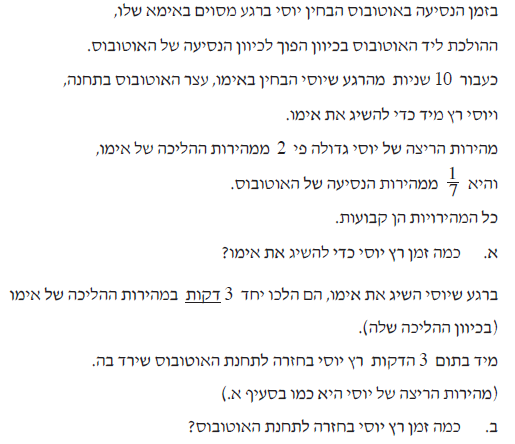
\includegraphics[width=.8\textwidth]{summer-2015b-1}
\end{center}

\vspace{-3ex}

\begin{center}
\selectlanguage{english}
\begin{tikzpicture}[scale=.85]
\draw (0,0) -- (14,0);
\draw (0,-4) node[left] {
\R{פרידה}
} -- (0,-2) node[left] {
\R{מפגש 2}
} -- (0,0) node[left] {
\R{מפגש 1}
} -- (0,4) node[left] {
\R{תחנה}
};
\fill (0,0) circle [radius=2pt];
\fill (1,0) circle [radius=2pt] node[below right] {$M$};
\fill (4,0) circle [radius=2pt] node[above] {$N$};
\fill (8,0) circle [radius=2pt] node[above] {$P$};
\fill (11,0) circle [radius=2pt] node[below right] {$Q$};
\fill (14,0) circle [radius=2pt] node[below] {$R$};
\draw[thick] (0,0) -- node[left] {$a$} (1,4) -- node[right,near start] {$b$} (4,-2);
\draw[thick] (0,0) -- node[below,near start,xshift=-2mm] {$c$} node[right,near end,yshift=2mm] {$d$} (8,-4)  node[below] {$P'$} -- (14,4)  node[right] {$R'$};
\draw[dashed] (0,4) -- (14,4);
\draw[dashed] (0,-2) -- (14,-2);
\draw[dashed] (0,-4) -- (14,-4);
\draw[dashed] (1,4)  node[above] {$M'$} -- (1,0);
\draw[dashed] (4,0) -- (4,-2) node[below,yshift=-1mm] {$N'$};
\draw[dashed] (8,-4) -- (8,0);
\draw[dashed] (11,0) -- (11,4);
\draw[dashed] (14,0) -- (14,4);
\draw[<->] (0,.7) -- node[fill=white] {$10$} (1,.7);
\draw[<->] (1,.7) -- node[near start,fill=white] {$t$} (4,.7);
\draw[<->] (4,.7) -- node[fill=white] {$180$} (8,.7);
\draw[<->] (8,.7) -- node[fill=white] {$t_1$} (11,.7);
\draw[<->] (11,.7) -- node[fill=white] {$t_2$} (14,.7);
\path (8,-2) --  node[below right,xshift=5mm,yshift=-2mm] {$e_1$} (11,0);
\path (11,0) --  node[left,yshift=3mm] {$e_2$} (14,4);
\end{tikzpicture}
\end{center}

\vspace{-3ex}

בתרשים סימנו את הקטעים:
\begin{center}
\begin{tabular}{rr}
\R{$=b$
יוסי רץ לפגישה עם אמא}
&
\R{$=a$
יוסי נוסע באוטובוס}\\
\R{$=d$
יוסי ואמא הולכים ביחד}
&
\R{$=c$
אמא הולכת עד למפגש עם יוסי}\\
&
\R{$=e_1+e_2$
יוסי רץ חזרה לתחנה}
\end{tabular}
\end{center}

\np

נסמן:
$=t$
הזמן שיוסי רץ מהתחנה כדי להשיג את אמא.

נסמן מהירויות:
$=v_y$
יוסי, 
$=v_a$
אמא, 
$=v_b$
אוטובוס.

נתון:
$v_y=2v_a$, $v_y=v_b/7$.

\medskip

\textbf{סעיף א}

את הזמן
$t$
נוכל לחשב ממשוואות התנועה מהמפגש הראשון )יוסי רואה את אימו( ועד למפגש השני )יוסי משיג את אימו(. המרחק מסומן
$NN'$
בתרשים. נוכל למצוא שתי משוואות עבור מרחק זה, אחד עבור אמא )קטע
$c$(:
\[
v_a(t+10),
\]
ואחד עבור יוסי )קטעים
$a,b$(:
\[
-v_b\cdot 10 + v_yt\,.
\]
שימו לב שבקטע 
$a$
יוסי 
\textbf{מתרחק}
מהמפגש ולכן המהירות שלילית.

נשווה את המרחקים ונציב את יחס המהירויות הנתון:
\erh{6pt}
\begin{equationarray*}{rcl}
 v_a(t+10)&=&v_yt -v_b\cdot 10\\
\frac{v_y}{2}(t+10)&=& v_yt - 7v_y 10\,.
\end{equationarray*}
הפתרון הוא
$150=t$
שניות.
\medskip

\textbf{סעיף ב}

מהתרשים קל לראות
\textbf{ששני}
קטעי הקווים
$e_1,e_2$
מתארים את הריצה של יוסי בחזרה לתחנה. רואים גם שהמרחק
$PP'$
של
$e_1$
הוא גם המרחק שאמא הולכת, קטעים 
$c,d$.
לפי התוצאה של סעיף א, לוקח לאמא
$10+150+180=340$
שניות לעבור מרחק זה. נתון שיוסי רץ פי שניים מהר יותר מההליכה של אמא, ולכן
$t_1=170$
שניות.

עבור הקטע השני
$e_2$,
המרחק
$RR'$
שווה למרחק
$MM'$,
המרחק שהאוטובוס עבר מהמפגש הראשון ועד התחנה. נתון שהאוטובוס עובר מרחק זה ב-%
$10$
שניות, ונתון שמהירות הריצה של יוסי פי שבע לאט ממהירות הנסיעה של האוטובוס, כך ש-%
$t_2=70$.

נסכם ונקבל שיוסי רץ מנקודת הפרידה לתחנה ב
$240=t_1+t_2$
שניות.

\bigskip

\textbf{שימו לב למלכודת:}
זמן ההליכה cיחד נתון בדקות ושאר הזמנים בשניות.

%%%%%%%%%%%%%%%%%%%%%%%%%%%%%%%%%%%%%%%%%%%%%%%%%%%%%%%%%%%%%%%%

\np

\section{קיץ תשע"ה מועד א}

\begin{center}
\selectlanguage{english}
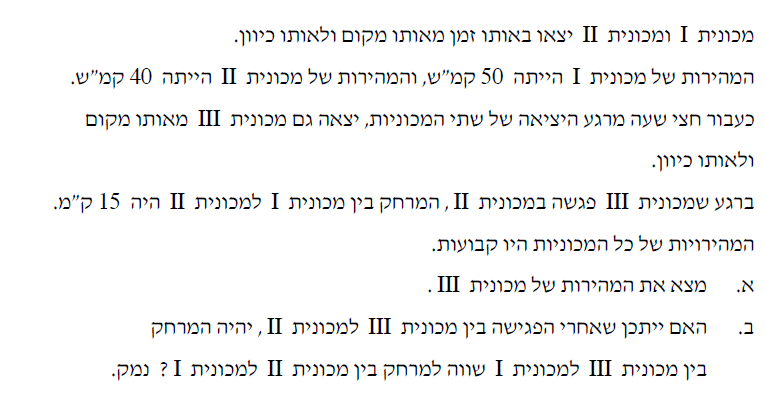
\includegraphics[width=.9\textwidth]{summer-2015a-1}
\end{center}

\begin{center}
\selectlanguage{english}
\begin{tikzpicture}[scale=1.2]
\draw (0,0) -- (10,0);
\draw (0,0) -- (0,6);
\draw[thick,name path=one] (0,0) -- node[below,near end,xshift=50pt,yshift=28pt] {I} (10,6);
\draw[thick,name path=two] (0,0) -- node[below,near end,xshift=50pt,yshift=14pt] {II} (10,3);
\draw[thick,name path=three] (3,0) -- node[above,near end,xshift=2pt,yshift=12pt] {III} (8,6);
\path [name intersections={of=one and three,by=one-three}];
\path [name intersections={of=two and three,by=two-three}];
\draw[dashed] (two-three) |- coordinate (time-two-three) (0,0);
\fill (0,0) circle [radius=2pt];
\fill (3,0) circle [radius=2pt];
\fill (one-three) circle [radius=2pt];
\fill (two-three) circle [radius=2pt];
\fill (time-two-three) circle [radius=2pt];
\node[above left] at (one-three) {$B$};
\node[below right] at (two-three) {$A$};
\path [name path=distance] (two-three) -| +(0,2);
\path [name intersections={of=one and distance,by=fifteen}];
\draw (two-three) -- (fifteen) node[above left] {
\R{ק"מ}
$15$};
\draw[->] (3.3,2.5) -- (3.8,1.7);
\fill (fifteen) circle [radius=2pt];
\draw[<->] (0,-.6) -- node[fill=white] {
\R{שעה}
 $1/2$} (3,-.6);
\draw[<->] (3,-.6) -- node[fill=white] {$t$} (time-two-three |- 0,-.6);
\end{tikzpicture}
\end{center}
המהירות של מכונית I גדולה מהמהירות של מכונית II, ולכן השיפוע שלו תלול יותר.

נסמן
$=t$
הזמן בין היציאה של III ועד למפגש שלו עם II,
$=v_3$
המהירות של III.

נתון: מהירות של I
$v_1=50$,
מהירות של II
$v_2=40$.

\textbf{סעיף א}

לאחר 
$t+1/2$
שעות, המכוניות II ו-III עברו אותו מרחק, ומכונית I עבר אותו מרחק ועוד 
$15$
ק"מ. נכתוב את משוואות התנועה לשני המקרים:
\begin{eqnarray*}
40(t+1/2) &=& v_3t\\
50(t+1/2) &=& v_3t + 15\,.
\end{eqnarray*}
מהמשוואות מתקבל
$t=1$
ואח"כ
$v_3=60$
קמ"ש.

\np

\textbf{סעיף ב}

נוסיף סימונים לתרשים שיעזרו לנו לפתור את הבעייה:

\begin{center}
\selectlanguage{english}
\begin{tikzpicture}[scale=1.2]
\draw (0,0) -- (10,0);
\draw (0,0) -- (0,6);
\draw[thick,name path=one] (0,0) -- node[below,near end,xshift=50pt,yshift=28pt] {I} (10,6);
\draw[thick,name path=two] (0,0) -- node[below,near end,xshift=50pt,yshift=14pt] {II} (10,3);
\draw[thick,name path=three] (3,0) -- node[above,near end,xshift=2pt,yshift=12pt] {III} (8,6);
\path [name intersections={of=one and three,by=one-three}];
\path [name intersections={of=two and three,by=two-three}];
\draw[dashed] (two-three) |- coordinate (time-two-three) (0,0);
\fill (0,0) circle [radius=2pt];
\fill (3,0) circle [radius=2pt];
\fill (one-three) circle [radius=2pt];
\fill (two-three) circle [radius=2pt];
\fill (time-two-three) circle [radius=2pt];
\node[above left] at (one-three) {$B$};
\node[below right] at (two-three) {$A$};
\path [name path=distance] (two-three) -| +(0,2);
\path [name intersections={of=one and distance,by=fifteen}];
\draw (two-three) -- (fifteen) node[above left] {
\R{ק"מ}
$15$};
\draw[->] (3.3,2.5) -- (3.8,1.7);
\fill (fifteen) circle [radius=2pt];
\draw[<->] (0,-.6) -- node[fill=white] {
\R{שעה}
 $1/2$} (3,-.6);
\draw[<->] (3,-.6) -- node[fill=white] {$t$} (time-two-three |- 0,-.6);
\draw[->] (4.5,3.2) -- +(.45,-.55);
\draw[<->,thick,densely dotted] (5.3,3.1) -- +(0,-1.5);
\draw[<->,thick,densely dotted] (5,2.95) -- +(0,-.5);
\node at (5.6,2.4) {I-II};
\node at (4.5,3.4) {I--III};
\draw[<->,thick,densely dotted] (7.8,4.6) -- node[right] {I--II} +(0,-2.2);
\draw[<->,thick,densely dotted] (7.8,4.8) -- node[right,yshift=3pt] {I--III} +(0,.8);
\end{tikzpicture}
\end{center}

נעיין בקווים מנוקדים בתרשים ונראה שהמרחקים לא יכולים שווים. בנקודה
$A$
הרחקים שווים, אבל מנקודה זו ועד לנקודה
$B$,
המרחק I--II גדל והמרחק I--III קטן.

בנקודה
$B$
המרחק I--II חיובי והמרחק I--III שווה לאפס. מכאן והלאה, שני המרחקים גדלים באותו קצב כי הפרשי המהירויות שווים:
$10=60-50=50-40$
קמ"ש.

\smallskip

\textbf{הוכחה בחישוב}

נסמן
$=t_A$
זמן מנקודה
$A$,
$=t_B$
זמן מנקודה
$B$,
$=d_B$
המרחק בין I ל-II בנקודה
$B$.

\smallskip

משמאל לנקודה
$B$
המרחקים שווים
\textbf{אם}:
\[
15 + (v_1-v_2)t_A \stackrel{?}{=} 15 + (v_1-v_3)t_A\,.
\]
נציב
$v_1=50, v_2=40, v_3=60$
ונקבל
$10=-10$,
כך הטיעון לא יכול להיות נכון.

\smallskip

מימין לנקודה
$B$
המרחקים שווים
\textbf{אם}:
\[
(v_3-v_1)t_B \stackrel{?}{=} d_B + (v_1-v_2)t_B\,.
\]
לאחר הצבה עבור המהירויות, נקבל שהטיעון נכון אם
$d_B=0$,
אבל אנחנו יודעים ש-%
$d_B > 15$.

%%%%%%%%%%%%%%%%%%%%%%%%%%%%%%%%%%%%%%%%%%%%%%%%%%%%%%%%%%%%%%%%

\np

\section{חורף תשע"ה}

\begin{center}
\selectlanguage{english}
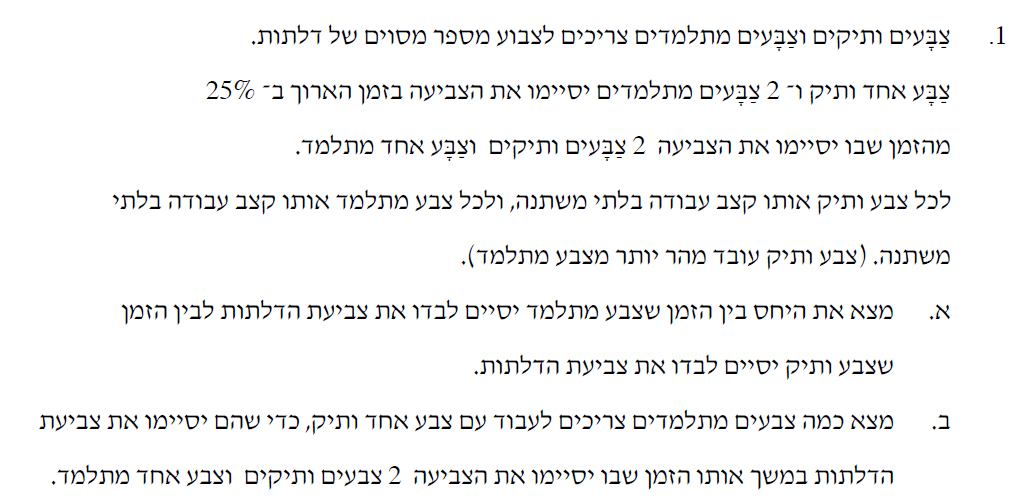
\includegraphics[width=\textwidth]{winter-2015-1}
\end{center}

\vspace{-2ex}

\textbf{סעיף א}

\begin{center}
\selectlanguage{english}
\begin{tikzpicture}
\draw (0,0) -- (10,0);
\draw (0,0) node[above left] {\R{אף דלת לא נצבע}}
-- (0,6) node[left] {\R{כל הדלתות נצבעו}};
\draw[dashed] (0,6) -- (10,6);
\draw[ultra thick] (0,0) -- node[left,near end,xshift=-2mm] {$2/t_v$} (8,4.5)  coordinate (two-one);
\draw[ultra thick] (0,4.5)  -- node[left,xshift=-2mm,yshift=2mm] {$1/t_m$} (8,6) coordinate (two-one-finish);
\draw[dotted,ultra thick] (0,4.5) -- (8,4.5);
\draw[thick] (0,0) -- node[left,yshift=2mm] {$1/t_v$} (10,2.25)  coordinate (one-two);
\draw[thick] (0,2.25)  -- node[left,near start,yshift=2mm] {$2/t_m$} (10,6) coordinate (one-two-finish);
\draw[dotted,thick] (0,2.25) -- (10,2.25);
\draw[dashed] (two-one-finish) -- (two-one-finish |- 0,0);
\draw[dashed] (one-two-finish) -- (one-two-finish |- 0,0);
\draw[<->] (0,-.6) -- node[fill=white] {$T$} (two-one-finish |- 0,-.6);
\draw[<->] (0,-1.2) -- node[fill=white] {$1.25 T$} (one-two-finish |- 0,-1.2);
\end{tikzpicture}
\end{center}
\vspace{-1ex}

נסמן את הזמנים לצביעת כל הדלתות: 
$=t_v$
צבע ותיק,
$=t_m$
צבע מתלמד.

השאלה שואלת על יחס בין זמנים, ולכן אין חשיבות לזמן הכולל לצביעות כל הדלתות. 
נסמן
$=1$
הזמן הכולל של שני ותיקים ומתלמד אחד, ו-%
$=1.25$
הזמן הכולל של שני מתלמדים וותיק אחד.

\smallskip

\noindent\textbf{הסבר על התרשים}

הצבעים עובדים במקביל אבל הציר בתרשים מראה
\textbf{חלוקת העבודה},
כאילו שצבע )או זוג צבעים( מסיים את חלקו בעבודה ואחר כך הצבע )או הזוג( השני מתחיל את חלקו. כאשר יש זוג צבעים הם רשומים כצבע אחד עם הספק כפול. הקווים הדקים מראים צבע אחד ותיק 
$(1/t_v)$
ושני צבעים מתלמדים
$(2/t_m)$.
הקווים העבים מראים שני צבעים ותיקים
$(2/t_v)$
וצבע אחד מתלמד
$(1/t_m)$.

\np

שני ההרכבים סיימו את כל העבודה, ומכאן שמשוואות ההספק נותנות אותו ערך:
\[
\frac{2}{t_v}\cdot 1 \:+\: \frac{1}{t_m}\cdot 1 \;=\; \frac{1}{t_v}\cdot 1.25 \:+\: \frac{2}{t_m} \cdot 1.25 \,.
\]
הפתרון הוא:
\[
\frac{t_m}{t_v}=2\,.
\]

\textbf{סעיף ב}

\begin{center}
\selectlanguage{english}
\begin{tikzpicture}
\draw (0,0) -- (10,0);
\draw (0,0) node[above left] {\R{אף דלת לא נצבע}}
-- (0,6) node[left] {\R{כל הדלתות נצבעו}};
\draw[dashed] (0,6) -- (10,6);
\draw[ultra thick] (0,0) -- node[left,near end,xshift=-2mm] {$2/t_v$} (8,4.5)  coordinate (two-one);
\draw[ultra thick] (0,4.5)  -- node[left,xshift=-2mm,yshift=2mm] {$1/t_m$} (8,6) coordinate (two-one-finish);
\draw[dashed,ultra thick] (0,4.5) -- (8,4.5);
\draw[thick] (0,0) -- node[left,yshift=2mm] {$1/t_v$} (8,2.25)  coordinate (one-two);
\draw[thick] (0,2.25)  -- node[left,near start,yshift=2mm] {$n/t_m$} (8,6) coordinate (one-two-finish);
\draw[dashed,blue] (0,2.25) -- (8,2.25);
\draw[dashed] (two-one-finish) -- (two-one-finish |- 0,0);
\draw[<->] (0,-.6) -- node[fill=white] {$1$} (two-one-finish |- 0,-.6);
\end{tikzpicture}
\end{center}

נסמן
$=n$
מספר הבצעים המתלמדים. העבודה של שני ההרכבים שווה ולכן:
\[
\frac{2}{t_v} + \frac{1}{t_m} = \frac{1}{t_v} + \frac{n}{t_m}\,.
\]
נשתמש ביחס שחישבנו בסעיף א ונקבל:
\[
n = \frac{t_m}{t_v}+1 = 2+1=3\,.
\]

%%%%%%%%%%%%%%%%%%%%%%%%%%%%%%%%%%%%%%%%%%%%%%%%%%%%%%%%%%%%%%%%

\np

\section{קיץ תשע"ד מועד ב}

\begin{center}
\selectlanguage{english}
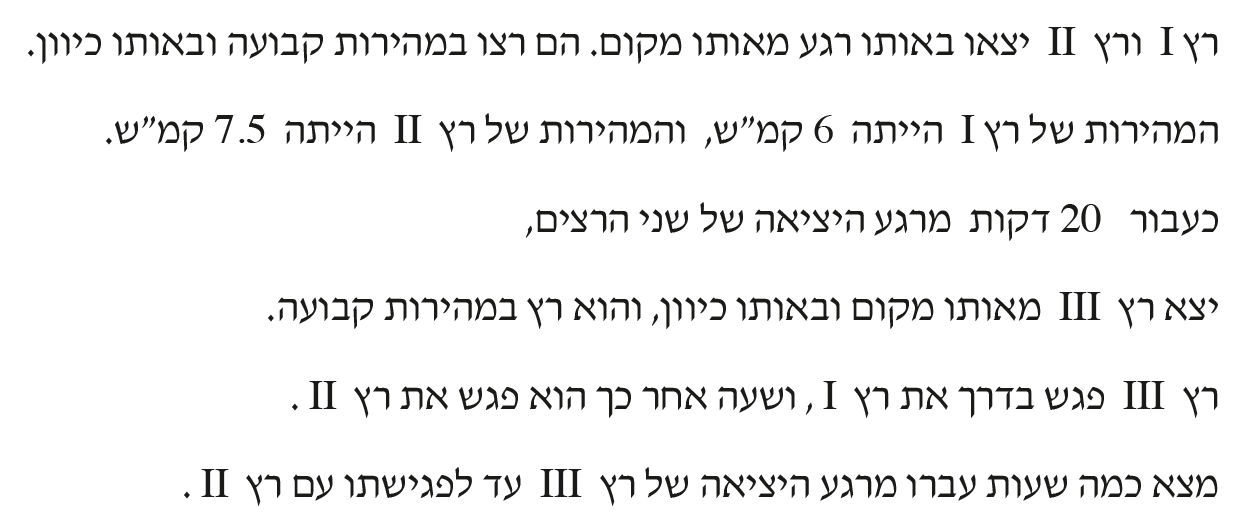
\includegraphics[width=.9\textwidth]{summer-2014b-1}
\end{center}

\begin{center}
\selectlanguage{english}
\begin{tikzpicture}
\draw (0,0) -- (10,0);
\draw (0,0) -- (0,6);
\draw[thick,name path=one] (0,0) -- node[below,near end,xshift=4pt] {I} (10,4);
\draw[thick,name path=two] (0,0) -- node[below,near end,xshift=16pt,yshift=6pt] {II} (10,6);
\draw[thick,name path=three] (2,0) -- node[above,near end,yshift=6pt] {III} (9,6);
\path [name intersections={of=one and three,by=one-three}];
\path [name intersections={of=two and three,by=two-three}];
\draw[dashed] (one-three) |- coordinate (time-one-three) (0,0);
\draw[dashed] (two-three) |- coordinate (time-two-three) (0,0);
\fill (0,0) circle [radius=2pt];
\fill (2,0) circle [radius=2pt];
\fill (one-three) circle [radius=2pt];
\fill (two-three) circle [radius=2pt];
\fill (time-one-three) circle [radius=2pt];
\fill (time-two-three) circle [radius=2pt];
\draw[<->] (0,-.6) -- node[fill=white] {
\R{שעה}
 $1/3$} (2,-.6);
\draw[<->] (2,-.6) -- node[fill=white] {$t$} (time-one-three |- 0,-.6);
\draw[<->] (time-one-three |- 0,-.6) -- node[fill=white] {
\R{שעה}
 $1$} (time-two-three |- 0,-.6);
\end{tikzpicture}
\end{center}

נסמן:
$=t$
הזמן בין היציאה של III ועד למפגש עם I,
$=v$
המהירות של III.

נתון:
$=6$
מהירות של I ו-
$=7.5$
המהירות של II. שימו לב לשיפועים של הקווים.

בכל מפגש בין שתי דמויות המרחקים שעברו שווים. המפגש בין I ל-III:
\[
6(t+1/3) = vt\,,
\]
והמפגש בין II ו-III:
\[
7.5(1/3+t+1) = v(t+1)\,.
\]
מהמשוואה הראשונה נקבל ביטוי עבור 
$v$
ונציב במשוואה השנייה. נקבל משוואה ריבועית ב-%
$t$:
\[
1.5t^2 + 2t - 2 = 0\,,
\]
שיש לה פתרון חיובי אחד
$t=2/3$.

\smallskip

הזמן מהיציאה של III ועד המפגש עם II הוא
$t+1=5/3$
שעות.

%%%%%%%%%%%%%%%%%%%%%%%%%%%%%%%%%%%%%%%%%%%%%%%%%%%%%%%%%%%%%%%%

\np

\section{קיץ תשע"ד מועד א}

\begin{center}
\selectlanguage{english}
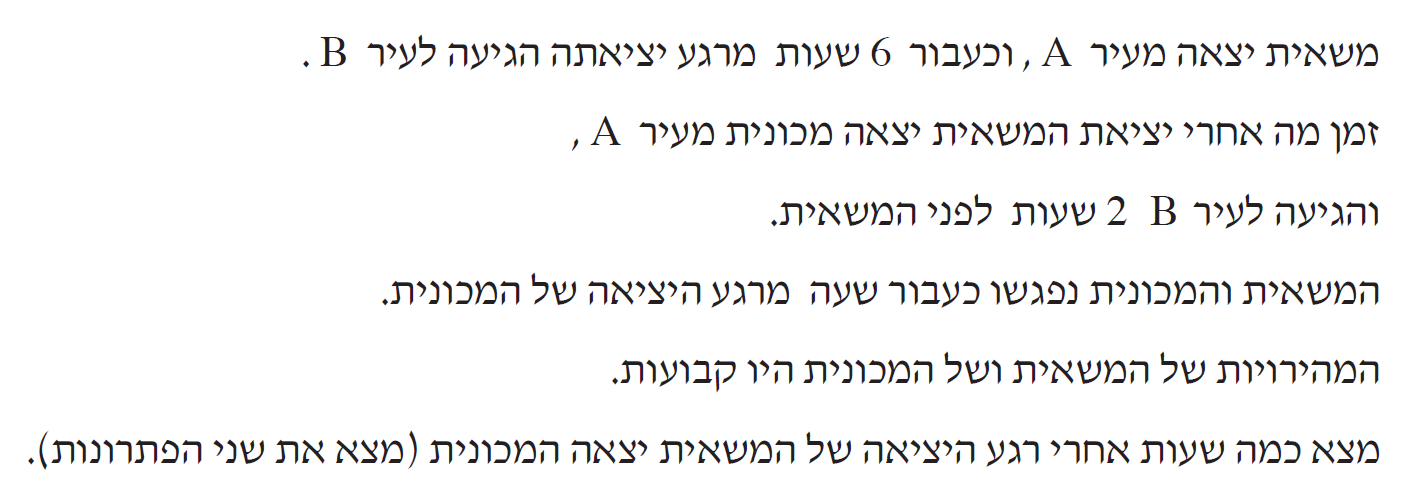
\includegraphics[width=\textwidth]{summer-2014a-1}
\end{center}

\begin{center}
\selectlanguage{english}
\begin{tikzpicture}
\draw (0,0) node[left] {$A$} -- (10,0);
\draw (0,0) -- (0,6) node[left] {$B$};
\draw[dashed] (0,6) -- (10,6);
\draw[thick,name path=truck] (0,0) -- node[left,near start,xshift=-6pt] {
\R{משאית}
} (10,6);
\draw[thick,name path=car] (3,0) -- node[left,near end] {
\R{מכונית}
} (7,6);
\path [name intersections={of=truck and car,by=meeting}];
\draw[dashed] (meeting) |- coordinate (time) (0,0);
\draw[dashed] (10,0) -- (10,6);
\draw[dashed] (7,0) -- (7,6);
\fill (meeting) circle [radius=2pt];
\fill (time) circle [radius=2pt];
\fill (0,0) circle [radius=2pt];
\fill (3,0) circle [radius=2pt];
\fill (7,0) circle [radius=2pt];
\fill (10,0) circle [radius=2pt];
\draw[<->] (0,-.5) -- node[fill=white] {$t$} (3,-.5);
\draw[<->] (3,-.5) -- node[fill=white] {
\R{שעה}
 $1$} (time |- 0,-.5);
\draw[<->] (time |- 0,-.5) -- node[fill=white] {$3-t$} (7,-.5);
\draw[<->] (7,-.5) -- node[fill=white] {
\R{שעות}
 $2$} (10,-.5);
\draw[<->] (3.1,-1.2) -- node[fill=white] {$4-t$} (6.9,-1.2);
\draw[<->] (0,-1.8) -- node[fill=white] {
\R{שעות}
 $6$} (10,-1.8);
\end{tikzpicture}
\end{center}

המפתח לפתרון הוא לסמן כל פרק זמן כפי שעשינו בתרשים.

נסמן:
$=t$
זמן יציאת המכונית,
$=v_c$
מהירות המכונית,
$=v_m$
מהירות המשאית.

\smallskip

נכתוב משוואות למרחקים שווים, מ-
$A$
עד למפגש ומ-
$A$
עד ל-
$B$:
\begin{eqnarray*}
v_m(t+1) &=& v_c\cdot 1\\
v_m \cdot 6 &=& v_c (4-t)\,.
\end{eqnarray*}
משתי המשוואות מתקבלת משוואה ריבועית ב-
$t$:
\[
t^2 - 3t + 2 = 0
\]
שיש לה שני פתרונות
$t=1$
שעה ו-
$t=2$
שעות.

%%%%%%%%%%%%%%%%%%%%%%%%%%%%%%%%%%%%%%%%%%%%%%%%%%%%%%%%%%%%%%%%

\np

\section{חורף תשע"ד}

\begin{center}
\selectlanguage{english}
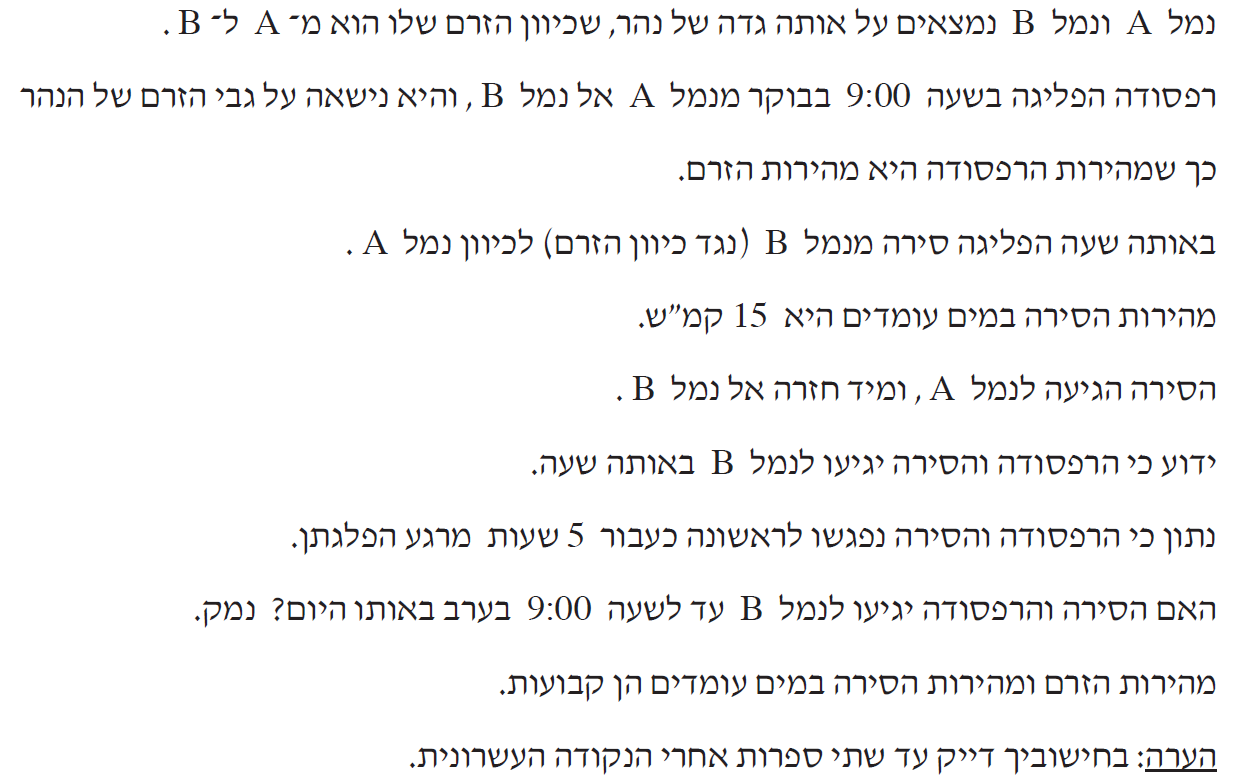
\includegraphics[width=\textwidth]{winter-2014-1}
\end{center}

\begin{center}
\selectlanguage{english}
\begin{tikzpicture}
\draw (0,0) node[below left] {$A$} node[below,xshift=-14pt,yshift=-10pt] {\p{9:00}} -- (10,0);
\draw (0,0) -- (0,6) node[above left] {$B$};
\draw[dashed] (0,6) -- (10,6);
\draw[thick,name path=raft] (0,0) -- node[left,near start,xshift=-4pt] {
\R{רפסודה}
} (10,6);
\draw[thick,name path=boat] (0,6) -- node[right,near start,xshift=2pt] {
\R{סירה}
} (8,0) -- (10,6);
\path [name intersections={of=boat and raft,by=meeting}];
\draw[dashed] (meeting) |- coordinate (time) (0,0);
\draw[dashed] (meeting) -| coordinate (distance) (0,0);
\draw[dashed] (8,0) -- (8,6);
\draw[dashed] (10,0) -- (10,6);
\fill (meeting) circle [radius=2pt];
\fill (time) circle [radius=2pt];
\fill (0,0) circle [radius=2pt];
\fill (8,0) circle [radius=2pt];
\fill (8,6) circle [radius=2pt];
\fill (10,6) circle [radius=2pt];
\fill (10,0) circle [radius=2pt];
\fill (distance) circle [radius=2pt];
\draw[<->] (-.4,0) -- node[fill=white] {$d_1$} (distance -| -.4,0);
\draw[<->] (distance -| -.4,0) -- node[fill=white] {$d_2$} (-.4,6);
\draw[<->] (-.9,0) -- node[fill=white] {$d$} (-.9,6);
\draw[<->] (0,-.6) -- node[above] {
\R{שעות}
 $5$} (time |- 0,-.6);
\draw[<->] (0,-1.2) -- node[fill=white] {$t_1$} (8,-1.2);
\draw[<->] (8,-1.2) -- node[fill=white] {$t_2$} (10,-1.2);
\draw[<->] (0,-1.8) -- node[fill=white] {$t$} (10,-1.8);
\end{tikzpicture}
\end{center}

\vspace{-2ex}

נסמן:
$=d$
מרחק בין שני הנמלים,
$=d_1$
מרחק בין
$A$
למפגש,
$=d_2$
מרחק בין 
$B$
למפגש.

$=t$
זמן עד למפגש ב-%
$B$,
$=v$
מהירות הזרם.

\smallskip

כאשר הסירה מפליגה מ-%
$B$
ל-%
$A$
ובחזרה ל-%
$B$,
היא עוברת מרחק כפול מהמרחק שהרפסודה עוברת באותו פרק זמן. נשווה את משוואות התנועה:

\np

\[
\frac{d}{v} = \frac{d}{15-v} + \frac{d}{15+v}\,.
\]
$d$
מצטמצם ונקבל משוואה ריבועית במהירות הזרם
$v$:
\[
v^2+30v-225=0\,.
\]
השורש החיובי שלה הוא
$v=6.21$.

\smallskip

עכשיו שאנחנו יודעים את המהירויות, והזמן עד למפגש נתון, ננסה לחשב את המרחק 
$d$,
שהוא הסכום של המרחקים שעוברים הרפסודה והסירה:
\[
d = 5v + 5(15-v)\,.
\]
הפתרון הוא
$d=75$
)ללא תלות במהירות הזרם
$v$(.

\smallskip

את הזמן עד המפגש בנמל 
$B$
אפשר לחשב לפי ההפלגה של הסירה או לפי ההפלגה של הרפסודה. כמובן שפשוט יותר לחשב עבור הקטע היחיד של הרפסודה:
\[
t = \frac{d}{v} = \frac{75}{6.21} \approx 12.08\,.
\]
בכל זאת נבדוק לפי הסירה:
\[
t = \frac{d}{15-v} + \frac{d}{15+v} = \frac{75}{8.79} + \frac{75}{21.21}= 8.532 + 3.536 \approx 12.07\,.
\]
בגלל עיגול של החישובים יש הבדל קטן בין שתי התוצאות.

הסירה והרפסודה יצאו בשעה
\L{\p{09:00}}
בבוקר וההפלגות לקחו יותר מ-%
$12$
שעות, כך המפגש השני התקיים לאחר השעה
\L{\p{09:00}}
בערב.


%%%%%%%%%%%%%%%%%%%%%%%%%%%%%%%%%%%%%%%%%%%%%%%%%%%%%%%%%%%%%%%%

\selectlanguage{english}
\clearpage
\selectlanguage{hebrew}


\section*{המלצות: תנועה והספק}

\addcontentsline{cot}{chapter}{המלצות: תנועה והספק}

\begin{itemize}

\item
בניגוד תרשימים חד-ממדיים האורך של קטע קו הוא מרחק הנסיעה, כאן מרחק הנסיעה הוא ההפרש בציר האנכי בין הנקודה ההתחלתית לנקודה הסופית. קטע הקו עצמו יהיה משופע ולכן יהיה אורך יותר ממרחק הנסיעה.

\item
הקושי בפתרון של הבעיות הללו נובע מהצורך לתרגם את התיאורים המילוליים למשוואת. אפשר בקלות להתבלבל כאשר מתרגמים ביטויים כגון "לפני", "אחרי", "מהר יותר", "לאט יותר".  בתרשים קל ליצג את התיאורים הללו: נקודות שהן "לפני" ו-"אחרי" נקודת ייחוס יוצגו שמאלה או ימינה מנקודת הייחוס בציר הזמן. קו המסמן מסלול "מהר יותר" יוצג עם שיפוע תלול יותר מקו המסמן מסלול "לאט יותר".

\item
מומלץ להכין תרשימים גדולים וברורים כדי שהסימנים שמוסיפים ממידע נתון או ממידע המתקבל מחישובים יהיו קריאים. לעתים, כדאי להכין תרשימים חדשים לכל סעיף כדי שמידע הנחוץ רק לסעיף אחד לא יקשה על עיון במידע הנחוץ לסעיף אחר.

\item
מצאתי שאפשר "לקרוא" את המשוואות ישירות מהתרשימים. לחילופין אפשר גם לסדר את הנתונים בטבלה כמקובל.

\item 
נקודות מפגש נוחות מאוד לכתיבת זוג משוואות תנועה עם אותם נעלמים. הזמנים האם אותם זמנים )לפעמים בתוספת קבוע(, והמרחקים שווים )אם הדמויות נוסעות בותו כיוון(, או שסכום המרחקים שווה למרחק בין נקודות הקצה )כאשר הדמויות נוסעות אחת כלפי השנייה(.

\item 
פתרון המשוואות עצמן הוא בדרך כלל קל: שני משוואות עם שני נעלמים, כאשר המשוואות שיש לפתור הן לינאריות או ריבועיות.

\end{itemize}
\selectlanguage{english}

\tikzsetfigurename{series}
% !TeX root = chapter-1-2-3.tex

\selectlanguage{hebrew}

\chapter{סדרות}


%%%%%%%%%%%%%%%%%%%%%%%%%%%%%%%%%%%%%%%%%%%%%%%%%%%%%%%%%%%%%%%%%%%

\section{קיץ תשע"ח מועד ב}

\begin{center}
\selectlanguage{english}
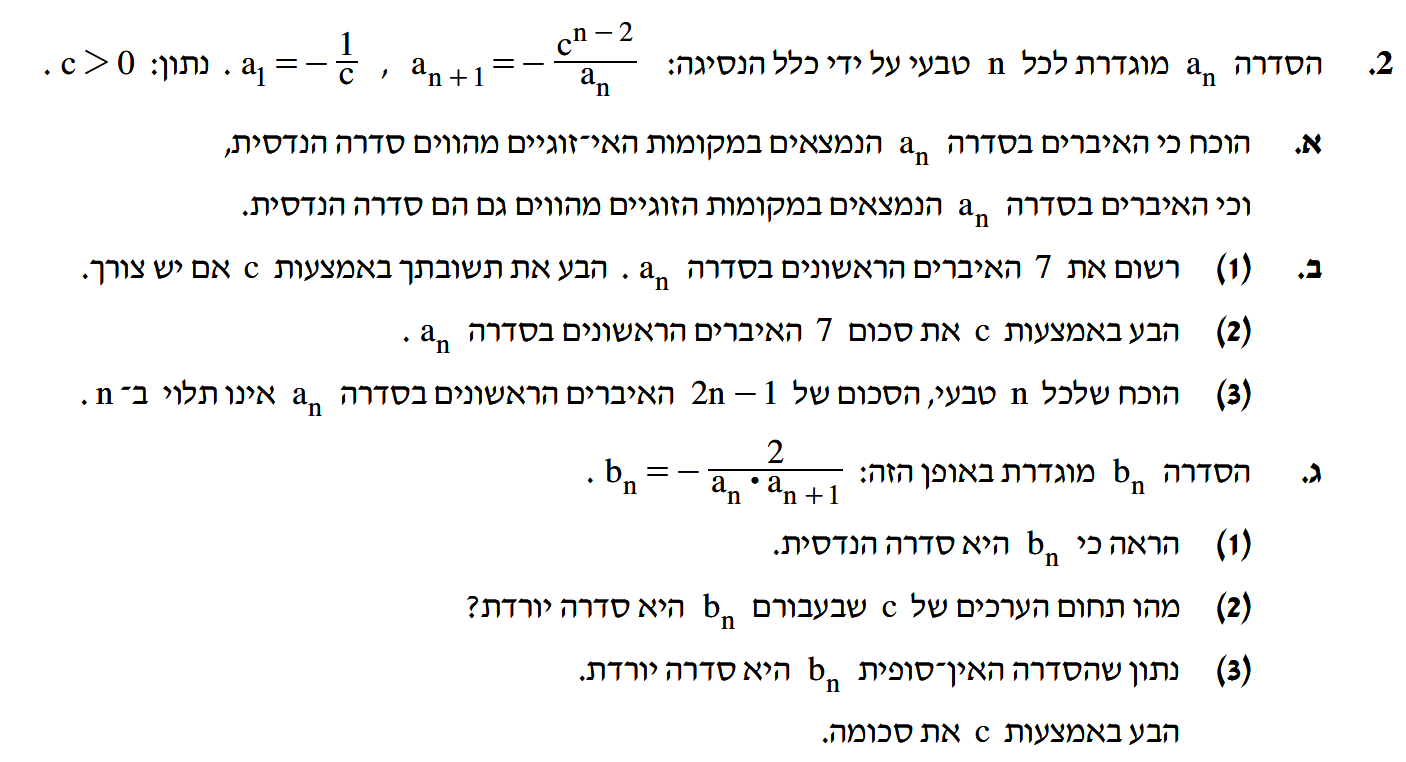
\includegraphics[width=\textwidth]{summer-2018b-2}
\end{center}
\vspace{-1ex}

\textbf{סעיף א}

כדי להוכיח שסדרה המוגדרת על ידי כלל נסיגה היא הנדסית, לא כדאי לחשב מנה של שני איברים עוקבים, כי איברים לא יצטמצמו. במקום זה, יש להציב את כלל הנסיגה כדי לקבל ערך של איבר כתלות של איבר אחר:
\[
a_{n+1} = -\frac{c^{n-2}}{a_n} = -\frac{c^{n-2}}{\displaystyle -\frac{c^{n-3}}{a_{n-1}}} = ca_{n-1}\,.
\]
המנה
$a_{n+1}/a_{n-1}=c$
קבועה ולא תלוי ב-%
$n$.
ההוכחה נכונה עבור כל זוג של איברים שיש הפרש של שניים במקומות שלהם בסדרה, ולכן ההוכחה נכונה גם עבור זוגות של מספרים זוגיים וגם עבור זוגות של מספרים א-זוגיים.

\smallskip

\textbf{סעיף ב}
$(1)$

הסדרות של הזוגיים והאי-זוגיים הן סדרות הנדסיות
\textbf{נפרדות}
ויש לחשב את האיברים בנפרד:

\vspace{-2ex}

\[
\erh{12pt}
\begin{array}{l}
a_1=-\displaystyle\frac{1}{c},\;\;a_3=ca_1=-1,\;\;a_5=ca_3=-c,\;\;a_7=ca_5=-c^2\\
a_2=\displaystyle
-\frac{c^{1-2}}{a_1}=
-\frac{c^{-1}}{-\frac{1}{c}}=1,\;\;a_4=ca_2=c,\;\;a_6=ca_4=c^2\,.
\end{array}
\]
שבעת האיברים הראשונים של הסדרה הם:
\[
-\frac{1}{c}\,,1\,, -1\,, c\,, -c\,, c^2\,, -c^2\,.
\]

\np

\textbf{סעיף ב}
$(2)$

כאשר מסכמים את האיברים הם מצטמצמים פרט לאיבר הראשון, ולכן
$S_7=-\frac{1}{c}$.

\smallskip

\textbf{סעיף ב}
$(3)$

כאשר יש מספר אי-זוגי של איברים המתחילים ממקום אי-זוגי, מספר האיברים האי-זוגיים גדול באחד ממספר האיברים הזוגיים. נבדוק דוגמה:
\[
a_1\,,a_2\,,a_3\,,a_4\,,a_5\,,a_6\,,a_7\,,a_8\,,a_9\,.
\]
מספר האיברים הוא
$9$,
מהם
$5$
אי-זוגיים ו-%
$4$
זוגיים.

נצטרך לסכם את זוגיים והאי-זוגיים בנפרד, כי הסדרה המקורית אינה הנדסית. עבור שתי התת-סדרות, המנה הוא 
$c$,
אבל האיבר הראשון שונה 
$-\frac{1}{c}, 1$:
\[
S_{\mathit{odd}}+S_{\mathit{even}}=-\frac{1}{c}\frac{c^n-1}{c-1}+ 1\cdot\frac{c^{n-1}-1}{c-1}=
%\frac{-c^{n-1}+c^{-1} + c^{n-1}-1}{c-1}=
-\frac{1}{c}\,,
\]
לא תלוי ב-%
$n$.

\smallskip

\textbf{סעיף ג}
$(1)$

כאן הסדרה נתונה על ידי נוסחה ולא כלל נסיגה ולכן ניתן לחשב ישירות את המנה:
\[
\frac{b_{n+1}}{b_n} = \frac{\displaystyle\frac{2}{a_{n+1}a_{n+2}}}{\displaystyle\frac{2}{a_{n}a_{n+1}}}= \frac{\displaystyle \frac{1}{a_{n+2}}}{\displaystyle \frac{1}{a_{n}}} =  \frac{1}{\displaystyle\frac{a_{n+2}}{a_n}} = \frac{1}{c}\,.
\]
\textbf{סעיף ג}
$(2)$

סדרה יורדת אם
$0<q=\displaystyle\frac{1}{c} < 1$.
נתון
$c>0$,
ולכן הסדרה יורדת אם
$c>1$.

\smallskip

\textbf{סעיף ג}
$(3)$

עבור סדרה הנדסית יורדת:
\erh{14pt}
\begin{equationarray*}{rcl}
S_b&=&\displaystyle\frac{b_1}{1-(1/c)}\\
&=&\frac{-2}{a_1\cdot a_{2}}\cdot \frac{c}{c-1}\\
&=&\frac{-2}{\displaystyle-\frac{1}{c}\cdot  1}\cdot \frac{c}{c-1}\\
&=&\frac{2c^2}{c-1}\,.
\end{equationarray*}

%%%%%%%%%%%%%%%%%%%%%%%%%%%%%%%%%%%%%%%%%%%%%%%%%%%%%%%%%%%%%%%%%%%
\np
\section{קיץ תשע"ח מועד א}

\begin{center}
\selectlanguage{english}
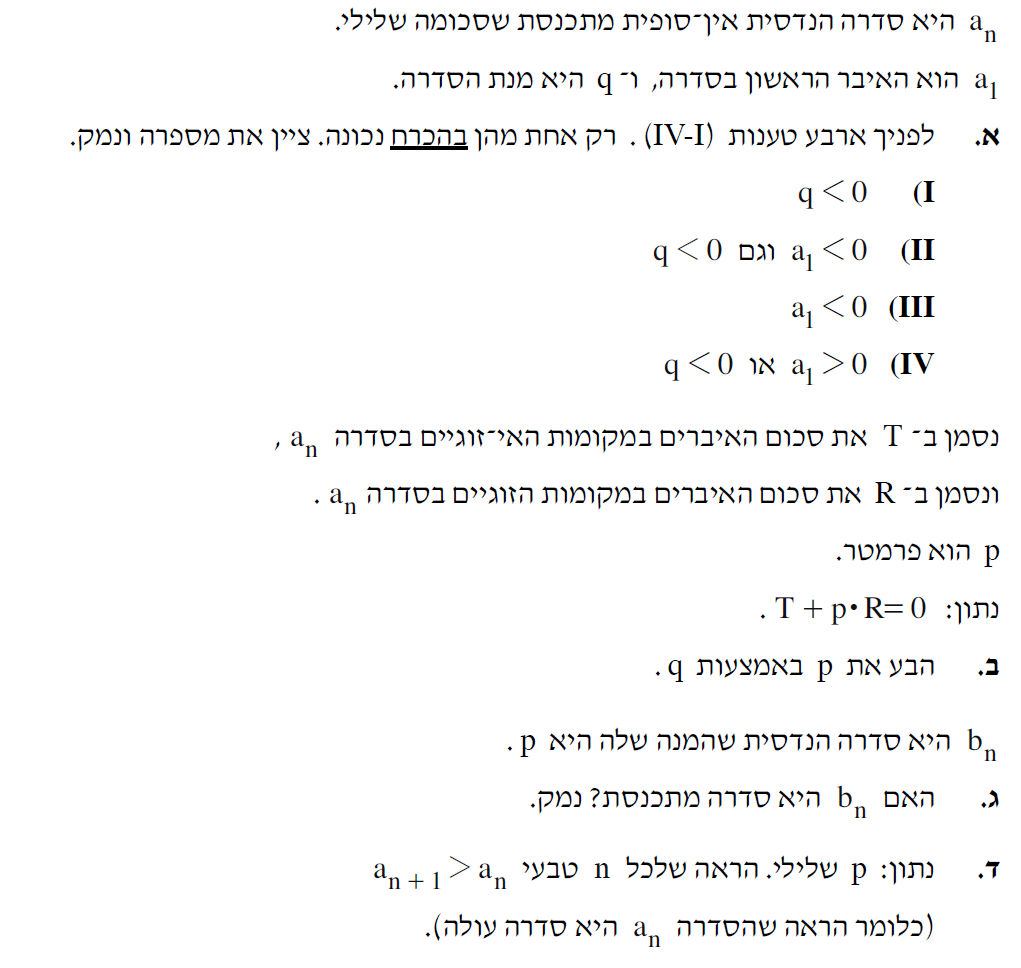
\includegraphics[width=.95\textwidth]{summer-2018a-2}
\end{center}

\textbf{סעיף א}

השאלה יפה כי היא דורשת חשיבה, לא חישובים! נבדוק את הטענות על סדרה מוכרת:
\[
1+ \frac{1}{2} + \frac{1}{4} + \frac{1}{8} + \cdots = 2\,.
\]
אם נהפוך את כל הסימנים למינוס, נקבל סדרה שסכומה שלילי:
\[
-1 - \frac{1}{2} - \frac{1}{4} - \frac{1}{8} - \cdots = -\left(1+ \frac{1}{2} + \frac{1}{4} + \frac{1}{8} + \cdots\right) = -2\,.
\]
ברור שהמנה עדיין חיובית:
\[
\frac{-2^{-(n+1)}}{-2^{-n}}=2^{-1}=\frac{1}{2}\,.
\]
לכן אפשר לפסול מייד תשובות 
\L{I, II, IV}
ונשאר רק תשובה
\L{III}.

\np

נעבור לסדרה כללית. סדרה הנדסית מתכנסת רק אם
$|q|<1$.
מהנוסחה עבור הסכום:
\[
S = \frac{a_1}{1-q} <0\,,
\]
ניתן לראות ש-% 
$a_1$
שלילי כי המכנה חיובי
$0 < 1-q < 2$.

\smallskip

\textbf{סעיף ב}

כאן מדובר בתת-סדרות של סדרה הנדסית, ועוד תת-סדרות שאיבריהן במקום קבוע אחד מהשני )הפרש של שני מקומות: זוגי לזוגי או אי-זוגי לאי-זוגי(. לכן, המנה של כל אחת מהסדרות היא
$q^2$,
והסכומים הם:
\[
T = \frac{a_1}{1-q^2},\quad\quad R = \frac{a_1q}{1-q^2}\,.
\]
מהמשוואה הנתונה
$T+pR=0$,
נקבל
$\quad 1+pq=0\quad$
ו-%
$p=-\displaystyle\frac{1}{q}\quad$.

\smallskip

\textbf{סעיף ג}

הסדרה לא מתכנסת כי 
$|q|<1$
גורר
$|p|>1$.

\smallskip

\textbf{סעיף ד}

שימו לב שהשאלה שואלת על
\textbf{הסדרה המקורית}
$a_n$
ולא על 
$b_n$!
נתון ש-%
$p$
שלילי ולכן
$q=-\displaystyle\frac{1}{p}$
חיובי. נתון שהסדרה מתכנסת ולכן
$0<q<1$.
מצאנו בסעיף א ש-%
$a_1$
שלילי ולכן
$a_{n+1}>a_n$,
כי מכפלה של מספר שלילי
$x$
עם מספר חיובי פחות מ-%
$1$
מקטינה את הערך המוחלט
$|x|$
ומורידה את
$-|x|$.

נבדוק בדוגמה: אם 
$a_n=-6,q=\frac{1}{2}$,
אז:
\[
a_{n+1} = a_nq = -6\cdot \frac{1}{2} = -3 \;> \; -6 =a_n\,.
\]


%%%%%%%%%%%%%%%%%%%%%%%%%%%%%%%%%%%%%%%%%%%%%%%%%%%%%%%%%%%%%%%%%%%

\np
\section{חורף תשע"ח}

\begin{center}
\selectlanguage{english}
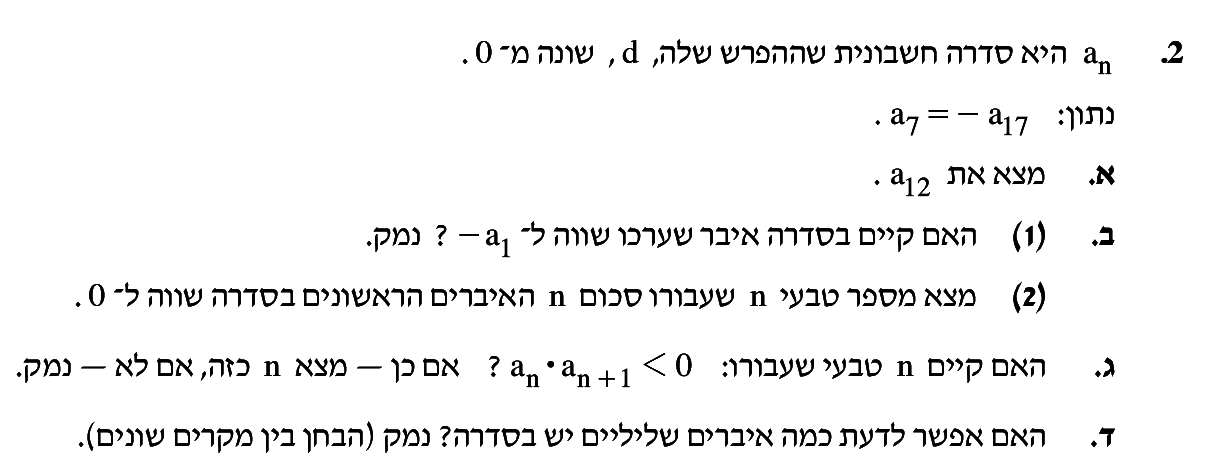
\includegraphics[width=.95\textwidth]{winter-2018-2}
\end{center}

\vspace{-1ex}

שאלה זו מתאפיין בהצבה של נוסחאות לאיברים מסויימים לתוך הנוסחאות הכלליות.

\smallskip

\textbf{סעיף א}

נציב 
$a_1+(n-1)d$
במשוואה
$a_7=-a_{17}$:
\[
\erh{2pt}
\begin{array}{l}
a_7=a_1+6d = -(a_1+16d)=-a_{17}\\
a_1+11d=0\\
a_{12}=a_1+11d=0\,.
\end{array}
\]
\textbf{סעיף ב}
$(1)$

נשווה את
$-a_1$
לנוסחה לאיבר כללי:
\[
-a_1 = a_n = a_1 + (n-1)d\,.
\]
נציב
$a_1=-11d$
שישבנו בסעיף א:
\[
-(-11d) = -11d + (n-1)d\,.
\]
$d$
מצטמצם ונקבל
$n=23$.

\smallskip

\textbf{סעיף ב}
$(2)$

נציב
$a_1=-11d$
 בנוסחה לסכום של סדרה חשבונית:
\[
\frac{n}{2}(2a_1+(n-1)d) = \frac{n}{2}(2\cdot -11d+(n-1)d) =\frac{dn}{2} (n-23)=0\,.
\]
%\begin{eqnarray*}
%0 &=& \frac{n}{2}(2a_1+(n-1)d)\\
%&=& \frac{n}{2}(2\cdot -11d+(n-1)d)\\
%&=& \frac{dn}{2} (n-23)\,.
%\end{eqnarray*}
נתון שההפרש 
$d$
שונה מאפס וש-%
$n$
מספר טבעי ולכן חיובי, כך שהביטוי מתאפס רק עבור
$n=23$.

\np

\textbf{סעיף ג}

אם איבר חיובי וההפרש חיובי, המכפלה של שני איברים עוקבים היא חיובית, וכך גם אם שניהם שליליים. האפשרות היחידה לקבל מכפלה שלילית היא איבר שלילי והפרש חיובי או איבר חיובי והפרש שלילי:
\[
\erh{2pt}
\begin{array}{l}
a_k<0,\; a_{k+1}>0\\
a_k>0,\; a_{k+1}<0\,.
\end{array}
\]
אבל ידוע שאחד האיברים בסדרה 
$(a_{12})$
הוא אפס:
\[
\erh{2pt}
\begin{array}{l}
a_k<0,\; a_{k+1}=0,\; a_{k+2}>0\\
a_k>0,\; a_{k+1}=0,\; a_{k+2}<0\,,
\end{array}
\]
ולכן המכפלה של זוג איברים עוקבים חייבת להיות חיובית או אפס.

\smallskip

\textbf{סעיף ד}

נרשום את הסדרה לפי מה שיודע לנו ש-%
$a_{12}=0$:
\[
a_1,\; a_2,\; \ldots,\; a_{11},\; 0,\; -a_{11},\; \ldots,\; -a_2,\; -a_1,\; \ldots\,.
\]
או ש-%
$11$
האיברים הראשונים שליליים אם ההפרש חיובי, או כל האיברים לאחר האיבר
$a_{12}=0$
שליליים אם ההפרש שלילי.



%%%%%%%%%%%%%%%%%%%%%%%%%%%%%%%%%%%%%%%%%%%%%%%%%%%%%%%%%%%%%%%%%%%
\np
\section{קיץ תשע"ז מועד ב}

\begin{center}
\selectlanguage{english}
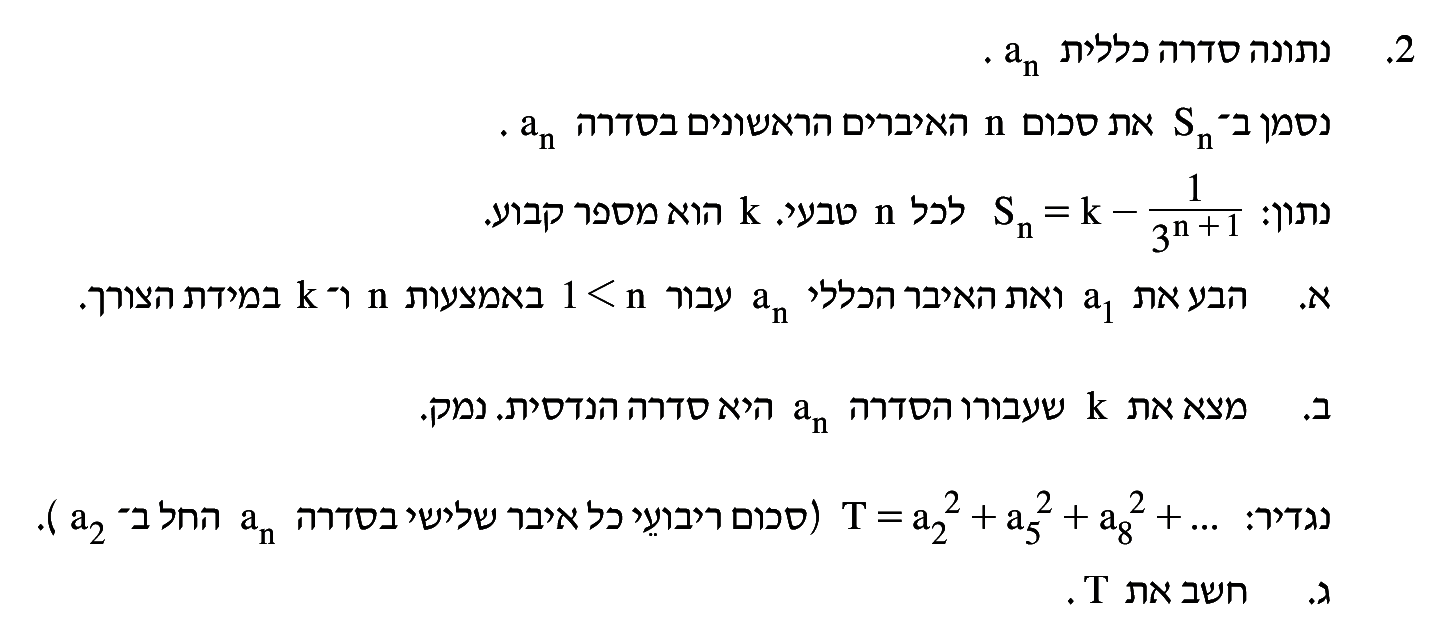
\includegraphics[width=.95\textwidth]{summer-2017b-2}
\end{center}

שאלה זו שונה משאלות אחרות כי נתון ביטוי עבור
\textbf{הסכומים}
ולא עבור האיברים בסדרה.

\smallskip

\textbf{סעיף א}

ניתן לחשב את האיברים על ידי שימוש בנוסחה עבור
$S_n$.
האיבר הראשון מתקבל ישירות מהנוסחה:
\[
a_1=S_1=k-\frac{1}{3^{1+1}}=k-\frac{1}{9}\,,
\]
והאיבר הכללי מתקבל על ידי ההפרש בין הנוסחאות לסכומים עוקבים:
\[
a_n=S_{n}-S_{n-1}=\left(k-\frac{1}{3^{n+1}}\right)-\left(k-\frac{1}{3^{n}}\right)=\frac{2}{3^{n+1}}\,.
\]
\textbf{סעיף ב}

המנה
$q=\displaystyle\frac{a_{n+1}}{a_{n}}=\frac{1}{3}$
לא תלויה ב-%
$k$.
במבט ראשון נראה שהתשובה היא שהסדרה היא הנדסית עבור כל ערך של
$k$,
אולם זו
\textbf{טעות}.
המנה המתקבלת מ-%
$\displaystyle\frac{a_2}{a_1}$
חייבת להיות
\textbf{שווה}
למנה המתקבלת מהמקרה הכללי
$\displaystyle\frac{a_{n+1}}{a_{n}}$.
נחשב:
\[
\frac{a_2}{a_1}=\frac{\displaystyle\frac{2}{3^3}}{\displaystyle k-\frac{1}{9}} =  \frac{2}{3(9k-1)} =\frac{a_{n+1}}{a_n}=\frac{1}{3}\,.
\]
הפתרון היחיד הוא
$\displaystyle k=\frac{1}{3}$.

עבור הסעיף הבא נצטרך את האיבר הראשון:
\[
\displaystyle \frac{1}{3}-\frac{1}{9}=\frac{2}{9}\,,
\]

\np

\textbf{סעיף ג}

האיבר הראשון בסדרה החדשה הוא:
\[
a'_1 = a_2^2=\left(a_1q\right)^2=\left(\frac{2}{9}\cdot\frac{1}{3}\right)^2=\frac{4}{729}\,,
\]
הסדרה החדשה היא הנדסית:
\[
\left(\frac{a_{3(k+1)-1}}{a_{3k-1}}\right)^2 =  \left(\frac{qa_{3k+1}}{a_{3k-1}}\right)^2=\left(\frac{q^2a_{3k}}{a_{3k-1}}\right)^2=\left(\frac{q^3a_{3k-1}}{a_{3k-1}}\right)^2=q^6=\left(\frac{1}{3}\right)^6=\frac{1}{729}\,.
\]
הסכום מתקבל מהנוסחה לסדרה הנדסית אינסופית עבור
$a', q'$:
\[
S'=\frac{a'_1}{1-q'}=
\frac{\displaystyle\frac{4}{729}}{1-\displaystyle\frac{1}{729}}= \frac{1}{182}\,.
\]

%%%%%%%%%%%%%%%%%%%%%%%%%%%%%%%%%%%%%%%%%%%%%%%%%%%%%%%%%%%%%%%%%%%
\np
\section{קיץ תשע"ז מועד א}

\begin{center}
\selectlanguage{english}
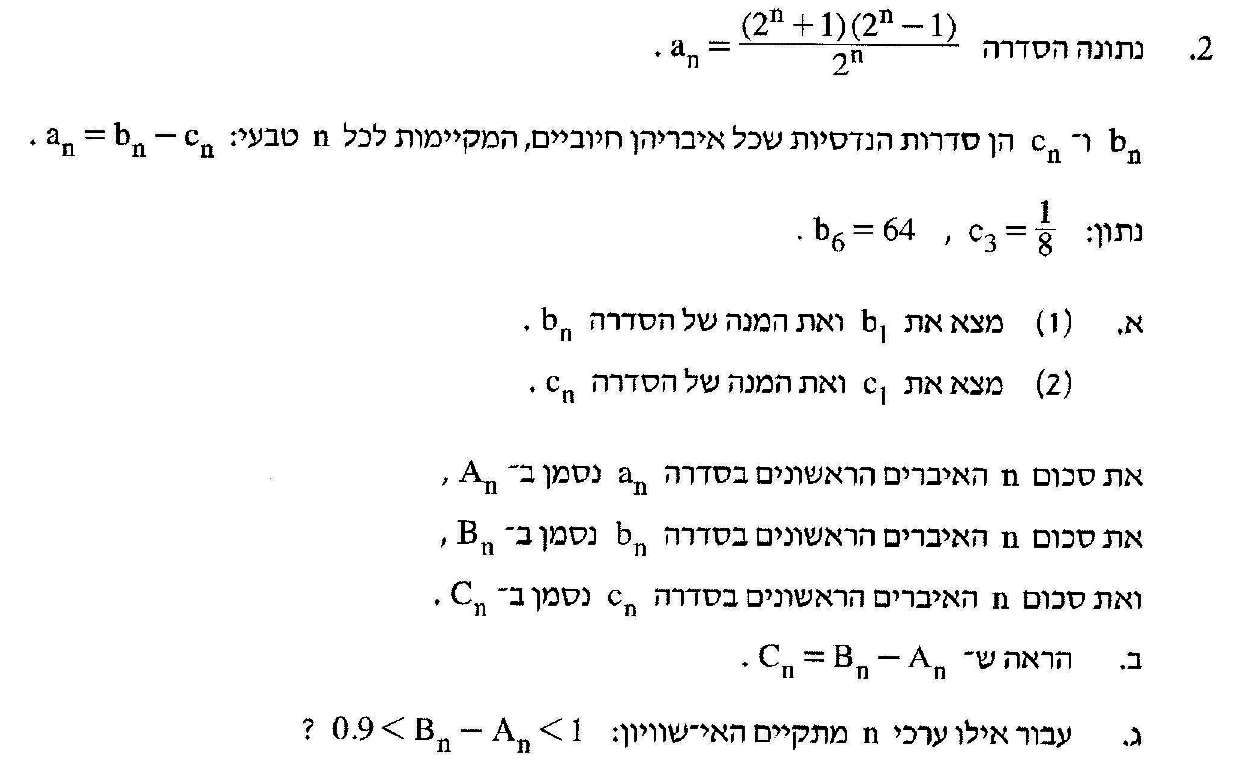
\includegraphics[width=.95\textwidth]{summer-2017a-2}
\end{center}
הנוסחה ל-%
$a_n$
אינה כלל נסיגה כי איברים של הסדרה לא מופיעים בצד הימני של המשוואה. נתון שהסדרות 
$b_n,c_n$
הנדסיות אך לא נתון אם הסדרה המקורית
$a_n$
הנדסית או לא.

\textbf{סעיף א}
$(1,2)$

נתון ש-%
$a_n=b_n-c_n$,
לכן כדי לקבל ערך של איבר בסדרה
$b_n$,
נצטרך לחשב את הערכים
$a_n,c_n$,
ובאופן דומה עבור איברים בסדרה
$c_n$.
נתון שני ערכים
$b_6,c_3$
וקל לחשב איברים ב-%
$a_n$
כי הם נתונים כפונקציה של 
$n$ 
בלבד:
\[
\erh{18pt}
\begin{array}{l@{\hspace{3em}}l}
\displaystyle a_3=\frac{(2^3+1)(2^3-1)}{2^3}=\frac{63}{8}&\displaystyle a_6=\frac{(2^6+1)(2^6-1)}{2^6}= \frac{65\cdot 63}{64}\\
\displaystyle b_3=a_3+c_3=\frac{63}{8}+\frac{1}{8}=8 &\displaystyle  c_6=b_6-a_6=64-\frac{65\cdot 63}{64}=\frac{1}{64}\,.
\end{array}
\]
כדי לחשב את מנה של
$b_n$
והמנה של
$c_n$
נשתמש בעבודה שהן סדרות הנדסיות וכדי לקבל את האיבר הששי מהאיבר השלישי יש להכפיל במנה לחזקת שלוש:
\vspace{-1ex}
\[
\erh{22pt}
\begin{array}{l@{\hspace{2em}}l@{\hspace{5em}}l@{\hspace{2em}}l}
b_6=b_3q_b^3 & \displaystyle q_b=\sqrt[3]{\frac{b_6}{b_3}}=\sqrt[3]{8}=2& b_3=b_1 q_b^2 & \displaystyle b_1=\frac{b_3}{q_b^2}=\frac{8}{4}=2\\
c_6=c_3q_c^3 & \displaystyle q_c=\sqrt[3]{\frac{c_6}{c_3}} =\sqrt[3]{\frac{1}{8}} = \frac{1}{2}& c_3=c_1 q_c^2 & \displaystyle c_1=\frac{c_3}{q_c^2}=\frac{1/8}{1/4}=\frac{1}{2}
\end{array}
\]

\np

\textbf{סעיף ב}

הטיעון נובע מחוקי הקיבוץ והחילוף של מספרים שלמים:
\begin{eqnarray*}
C_n &=& (b_1-a_1) + (b_2 - a_2) + \cdots + (b_n-a_n)\\
&=&(b_1 + b_2 + \cdots + b_n) - (a_1 + a_2 + \cdots + a_n)\\
&=& B_n - A_n\,.
\end{eqnarray*}
\textbf{סעיף ג}

הוכחנו ש-%
$C_n=B_n-A_n$,
ונתונה שהסדרה 
$c_n$
הנדסית. מסעיף א
$\displaystyle q_c=\frac{1}{2},\,c_1=\frac{1}{2}$,
ולכן:
\[
C_n = \frac{1}{2}\cdot\frac{\displaystyle\left(\left(\frac{1}{2}\right)^n-1\right)}{\displaystyle\left(\frac{1}{2}-1\right)}=1-2^{-n}\,.
\]
בדיקה במחשבון מראה ש:
%\vspace{-2ex}
\[
\erh{8pt}
\begin{array}{l}
0.9 \not< 1-2^{-3}=0.875<1\\
0.9 < 1-2^{-4}=0.938 < 1\,.
\end{array}
\]

לא לעצור כאן! השאלה מבקשת את
\textbf{כל הערכים}
של
$n$
המקיימים את האי-שוויון, ולכן התשובה המליאה היא כל מספר גדול או שווה ל-%
$4$,
כי כאשר 
$n$
גדל מעל ל-%
$4$,
הערך של 
$1-2^{-n}$
עולה )ולכן גדול מ-%
$0.9$(
אבל תמיד פחות מ-%
$1$.

%%%%%%%%%%%%%%%%%%%%%%%%%%%%%%%%%%%%%%%%%%%%%%%%%%%%%%%%%%%%%%%%%%%
\np
\section{חורף תשע"ז}

\begin{center}
\selectlanguage{english}
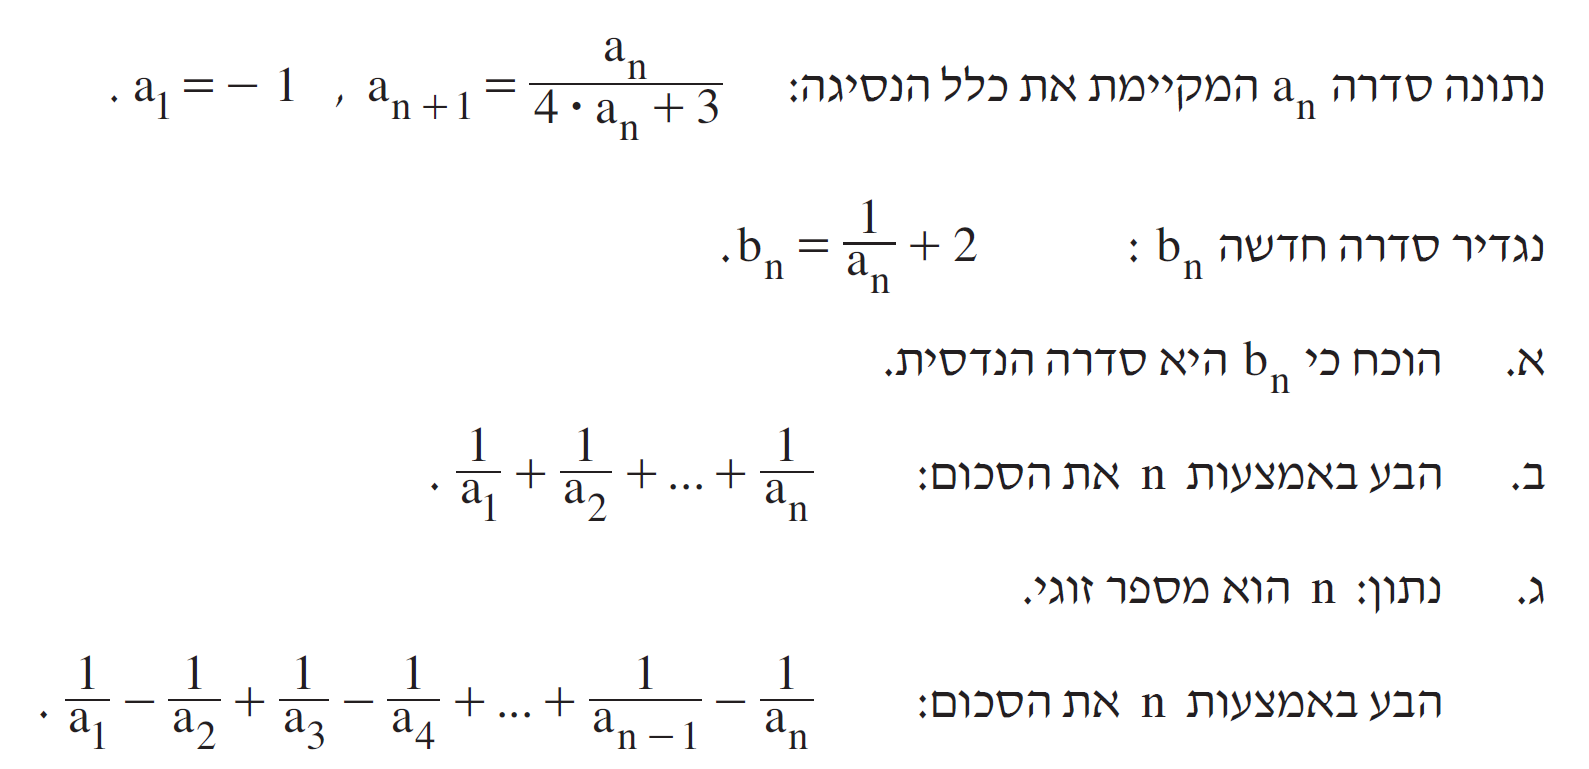
\includegraphics[width=.9\textwidth]{winter-2017-2}
\end{center}

\vspace{-2ex}

\textbf{סעיף א}

נחשב את המנה על ידי הצבה עבור 
$b_n$
לפי ההגדרה, ואחר כך הצבה עבור 
$a_{n+1}$
לפי כלל הנסיגה. נקבל מנה קבועה ולכן הסדרה הנדסית:
\[
\frac{b_{n+1}}{b_n} = \frac{\displaystyle\frac{1}{a_{n+1}}+2}{\displaystyle\frac{1}{a_{n}}+2}= \frac{\displaystyle\frac{4a_n+3}{a_n}+2}{\displaystyle\frac{1}{a_{n}}+2}=\frac{3(2a_n+1)}{2a_n+1}=3\,.
\]
\vspace{-3ex}

\textbf{סעיף ב}

לא נתון שהסדרה $a_n$ הנדסית, אבל בסעיף א הוכחנו שהסדרה  
$b_n$
הנדסית, ולכן ניתן לבטא את סכום הסדרה
$\displaystyle\frac{1}{a_n}$
כסכום של הסדרה
$b_n$
על ידי ההצבה 
$\displaystyle\frac{1}{a_i} = b_i - 2$:
\[
\frac{1}{a_1} + \cdots + \frac{1}{a_n}=(b_1-2) + \cdots + (b_n-2)=b_1+\cdots+b_n- 2n\,.
\]
נתון ש
$a_1=-1$,
כך ש-%
$b_1=\displaystyle\frac{1}{a_1}+2=1$
ובסעיף א חישבנו 
$q_b=3$.
סכום הסדרה של 
$\displaystyle \frac{1}{a_n}$
הוא:
\[
b_1+\cdots+b_n- 2n=\frac{1(3^n-1)}{3-1} - 2n = \frac{3^n - 4n -1}{2}\,.
\]
\textbf{סעיף ג}

לפי ההגדרה של 
$b_n$
נוכל לבטא את הסכום כך:
\[
(b_1 - 2) - (b_2 - 2) + \cdots + (b_{n-1} - 2) - (b_n - 2)\,.
\]
נתון שמספר האיברים זוגי ולכן סכום הקבועים מתאפס. המנה של הסדרה היא
$-3$
והסכום הוא:
\[
b_1-b_2+\cdots+b_{n-1}-b_n=\frac{1((-3)^n-1)}{-3-1}=\frac{(-3)^n-1}{-4}=\frac{1-3^n}{4}\,,
\]
כי מספר האיברים זוגי ולכן
$(-3)^n=3^n$.


%%%%%%%%%%%%%%%%%%%%%%%%%%%%%%%%%%%%%%%%%%%%%%%%%%%%%%%%%%%%%%%%%%%

\np
\section{קיץ תשע"ו מועד ב}

\begin{center}
\selectlanguage{english}
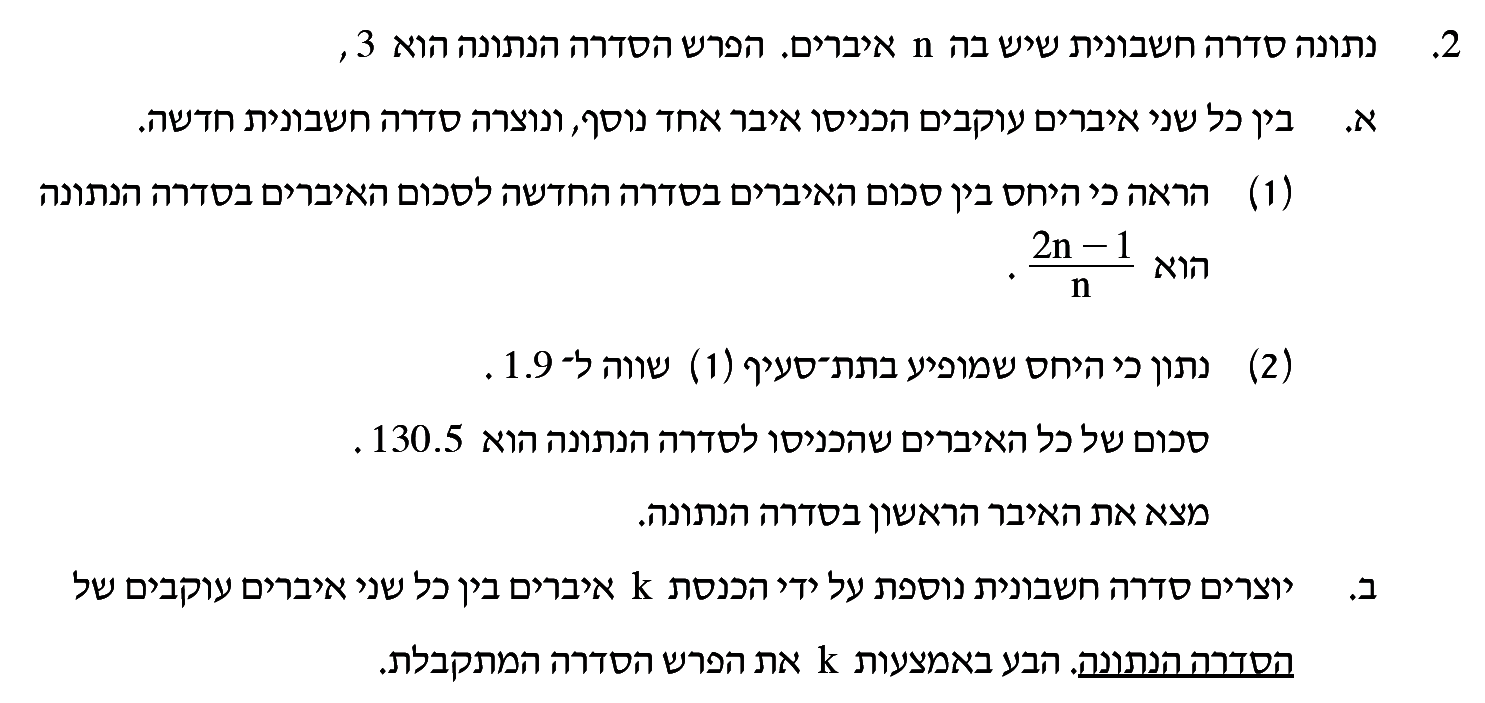
\includegraphics[width=.95\textwidth]{summer-2016b-2}
\end{center}
\vspace{-1ex}

\textbf{סעיף א}
$(1)$

מספר האיברים החדשים הוא
$n-1$,
כפי שרואים אם רושמים את הסדרה:
\[
a_1,\; a'_1,\; a_2,\; a'_2,\; \ldots,\; a_{n-1},\; a'_{n-1},\; a_n\,.
\]
נתון שהסדרה החדשה גם היא חשבונית. הפרש הסדרה אינו מספר שלם אלא
$1.5$!
אז מה? נחשב את היחס בין סכומי הסדרות, כאשר האיבר
$a_1$
מצטמצם:
\[
\frac{S_{\mathit{new}}}{S_{\mathit{old}}}= \frac{\displaystyle\frac{2n-1}{2}(2a_1+1.5(2n-1-1))}{\displaystyle\frac{n}{2}(2a_1+3(n-1))}=\frac{\displaystyle\frac{2n-1}{2}(2a_1+3(n-1))}{\displaystyle\frac{n}{2}(2a_1+3(n-1))}=\frac{2n-1}{n}\,.
\]
\textbf{סעיף א}
$(2)$

מ-%
$\displaystyle\frac{2n-1}{n}=1.9$
נקבל
$n=10$. 
אם הסדרה הנתונה חשבונית וגם הסדרה החדשה חשבונית, סדרת האיברים החדשים היא חשבונית עם אותו הפרש כמו בסדרה המקורית, 
$3$.
%
%נתון שהסדרה החדשה חשבונית ולכן גם סדרת האיברים החדשים חשבונית:
%\[
%a'_{i+1}-a'_{i}=a'_{i+1}-(a_{i+1}-a_{i+1})-a'_i=(a'_{i+1}-a_{i+1})+(a_{i+1}-a'_i)=\frac{d}{2}+\frac{d}{2}=3\,.
%\]
האיבר הראשון של האיברים החדשים הוא
$a'_1=a_1+1.5$,
ונתון סכום האיברים החדשים:
\[
\frac{10-1}{2}(2(a_1+1.5)+((10-1)-1)\cdot 3) = 130.5\,,
\]
והפתרון הוא
$a_1=1$.

\textbf{סעיף ב}

נתון שהסדרה המתקבלת לאחר הכנסת
$k$
איברים חדשים בין איברים סמוכים של הסדרה הנתונה:
\[
a_i,\; b_1,\; b_2,\; \ldots,\; b_k,\; a_{i+1}
\]
היא חשבונית. ההפרשים בין האיברים החדשים חייבים להיות שווים וסכומם שווה להפרש של הסדרה הנתונה שהוא
$3$.
יש
$k+1$
הפרשים שערכם
$\displaystyle\frac{3}{k+1}$.

%%%%%%%%%%%%%%%%%%%%%%%%%%%%%%%%%%%%%%%%%%%%%%%%%%%%%%%%%%%%%%%%%%%

\np
\section{קיץ תשע"ו מועד א}

\begin{center}
\selectlanguage{english}
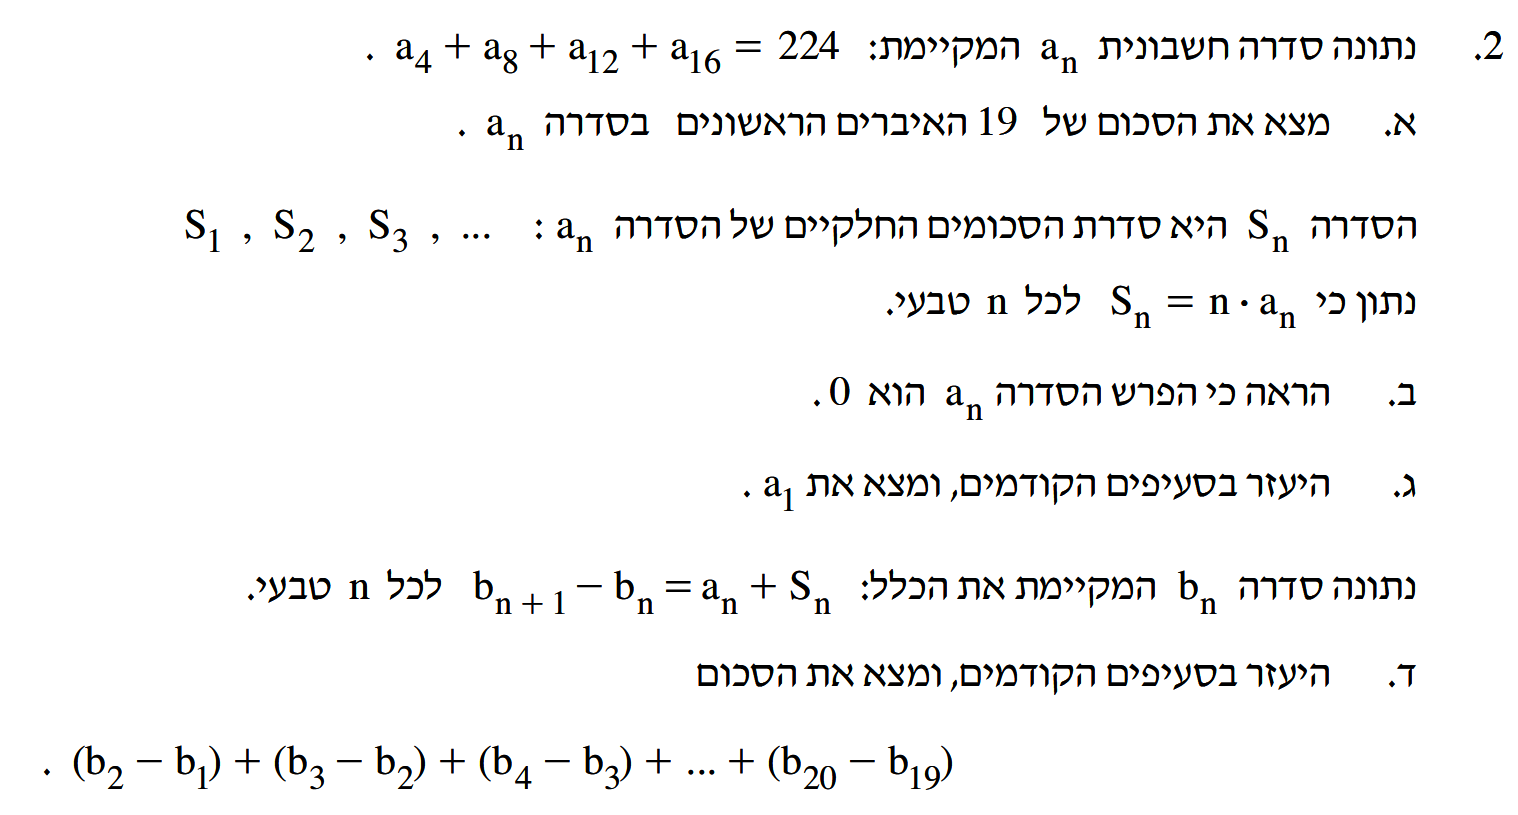
\includegraphics[width=.95\textwidth]{summer-2016a-2}
\end{center}
\vspace{-4ex}

\textbf{סעיף א}

האיברים
$a_4,a_8,a_{12},a_{16}$
מהווים סדרה חשבועית עם הפרש
$d^4$.
נתון הסכום של הסדרה:
\begin{eqnarray*}
(a_1+3d)+(a_1+7d)+(a_1+11d)+(a_1+15d)&=&224\\
a_1+9d&=&56\,.
\end{eqnarray*}
יש לנו משוואה אחת עם שני נעלמים. לא נתייאש וננסה בכל זאת לחשב את הסכום
$S_{19}$:
\[
S_{19}=\frac{19}{2}(2a_1+18d) = 19(a_1+9d)=19\cdot 56 = 1064\,.
\]
\vspace{-1ex}
\textbf{סעיף ב}

נשווה את המשוואה הנתונה
$S_n=n\cdot a_n$
לנוסחה עבור סכום של סדרה חשבונית:
\erh{10pt}
\begin{equationarray*}{rcl}
n\cdot a_n &=& \frac{n}{2}(2a_1+(n-1)d)\\
n(a_1+(n-1)d) &=&\frac{n}{2}(2a_1+(n-1)d)\,.
\end{equationarray*}
נפשט את המשוואה ונקבל 
$d=d/2$
שהפתרון היחיד שלה הוא
$d=0$.

\textbf{סעיף ג}

נציב
$0$
עבור 
$d$:
$a_1+9d=a_1+0=56$.

\textbf{סעיף ד}

במבט ראשון נראה שכדאי לצמצם את סכום הסדרה  ל-%
$b_{20}-b_1$,
אבל זה מבוי סתום כי אין לנו דרך לחשב את איברי הסדרה
$b_n$.
במקום זה נחשב את 
$(b_{i+1}-b_i)$
וניעזר במשוואה הנתונה:
\[
b_{i+1}-b_i=a_i+S_i=(a_1+(i-1)\cdot 0)+\frac{i}{2}(2a_1+(i-1)\cdot 0)=a_1(1+i)\,.
\]
הסכום הוא:
\[
a_1(2+3+\cdots+20)=56\cdot\frac{19}{2}(2\cdot 2 + (19-1)\cdot 1)=11704\,.
\]

%%%%%%%%%%%%%%%%%%%%%%%%%%%%%%%%%%%%%%%%%%%%%%%%%%%%%%%%%%%%%%%%%%%
\np
\section{חורף תשע"ו}

\begin{center}
\selectlanguage{english}
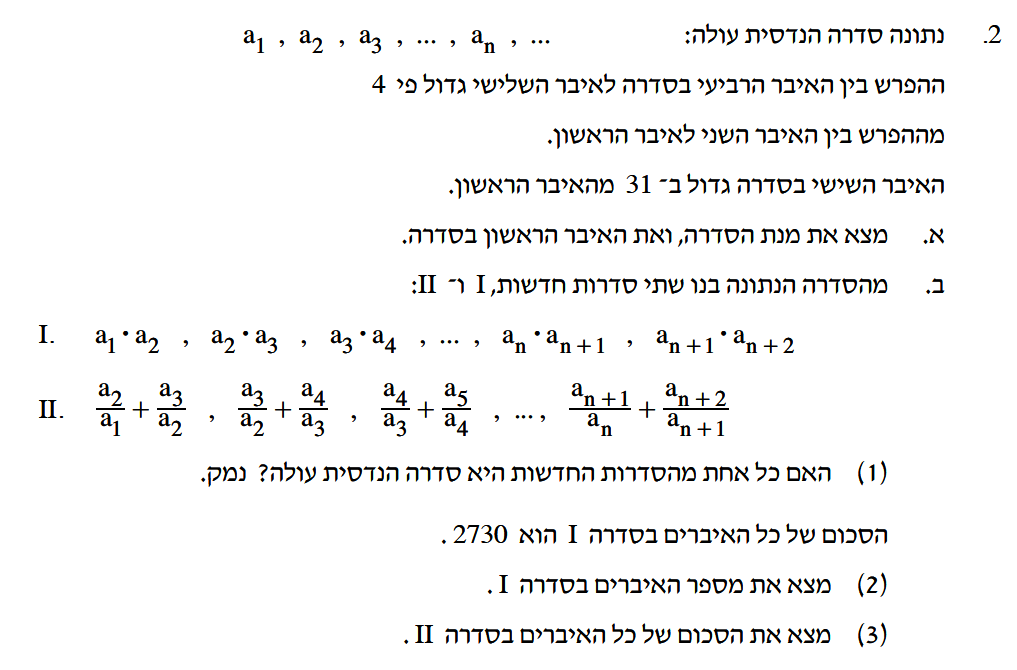
\includegraphics[width=.95\textwidth]{winter-2016-2}
\end{center}

\vspace{-3ex}

\textbf{סעיף א}

נתון:
\[
(1)\, a_4-a_3 = 4 (a_2-a_1),\quad (2)\, a_6 - a_1 = 31\,.
\]
נציב
$a_n=a_1q^{n-1}$ 
עבור
$a_2, a_3, a_4$,
ב-%
$(1)$,
ונקבל שלוש תשובות
$q=1,q=2,q=-2$.\\
נתון שהסדרה 
\textbf{עולה}
ולכן
$q=2$.
נציב 
$a_1q^5=32 a_1$
עבור
$a_6$
ב-%
$(2)$,
ונקבל
$a_1=1$.

\textbf{סעיף ב} 
$(1)$

עבור סדרה I:
\[
q_I=\frac{a_{n+1}\cdot a_{n+2}}{a_n\cdot a_{n+1}}=\frac{a_{n+2}}{a_n}=\frac{a_n\,q^2}{a_n}=q^2=4\,,
\]
והסדרה היא סדרה הנדסית עולה. עבור סדרה II:
\[
q_{II}=\left(\frac{a_{n+1}}{a_n} + \frac{a_{n+2}}{a_{n+1}}\right) / \left(\frac{a_{n}}{a_{n-1}} + \frac{a_{n+1}}{a_{n}}\right)=\frac{q+q}{q+q}=1\,.
\]
הסדרה הנדסית אבל
\textbf{לא עולה}.

\textbf{סעיף ב}
$(2)$

מסכום הסדרה ניתן לחשב את מספר האיברים בסדרה:
\begin{eqnarray*}
a_1\cdot a_2 + \cdots + a_{n+1} \cdot a_{n+2} &=& 2730\\
(1\cdot 2)\cdot \frac{4^{n+1}-1}{4-1}&=&2730\\
4^{n+1}&=&4096\\
n&=&5\,.
\end{eqnarray*}

\np

\textbf{שימו לב!}
אמנם
$n=5$
אבל מספר האיברים בסדרה I הוא 
$n+1=6$:
\[
(1)\, a_1\cdot a_2,\;\; (2)\,a_2\cdot a_3,\;\;(3)\, a_3\cdot a_4,\;\; (4)\,a_4\cdot a_5,\;\; (5)\,a_5\cdot a_6,\;\; (6)\,a_6\cdot a_7 \;(= a_{n+1}\cdot a_{n+2})\,.
\]
\textbf{סעיף ב}
$(2)$

חישבנו
$q_{II}=1$.
נחשב את
$a_1^{II}$:
\[
a_1^{II}=\frac{a_{2}}{a_1} + \frac{a_{3}}{a_{2}}=\frac{2}{1}+\frac{4}{2}=4\,.
\]
\textbf{שימו לב!}
מספר האיברים בסדרה II הוא 
$5$:
\[
(1)\,\frac{a_2}{a_1}+\frac{a_3}{a_2},\;\;
(2)\,\frac{a_3}{a_2}+\frac{a_4}{a_3},\;\;
(3)\,\frac{a_4}{a_3}+\frac{a_5}{a_4},\;\;
(4)\,\frac{a_5}{a_4}+\frac{a_6}{a_5},\;\;
(5)\,\frac{a_6}{a_5}+\frac{a_7}{a_6} \left(= \frac{a_{n+1}}{a_n}+\frac{a_{n+2}}{a_{n+1}}\right)\,.
\]
ולכן סכום האיברים הוא:
\[
a_1^{II}+a_1^{II}\cdot 1 + a_1^{II}\cdot 1^2 + \cdots + a_1^{II}\cdot 1^4 = 4\cdot 5=20\,.
\]


%%%%%%%%%%%%%%%%%%%%%%%%%%%%%%%%%%%%%%%%%%%%%%%%%%%%%%%%%%%%%%%%%%%
\np

\section{קיץ תשע"ה, מועד ב}

\begin{center}
\selectlanguage{english}
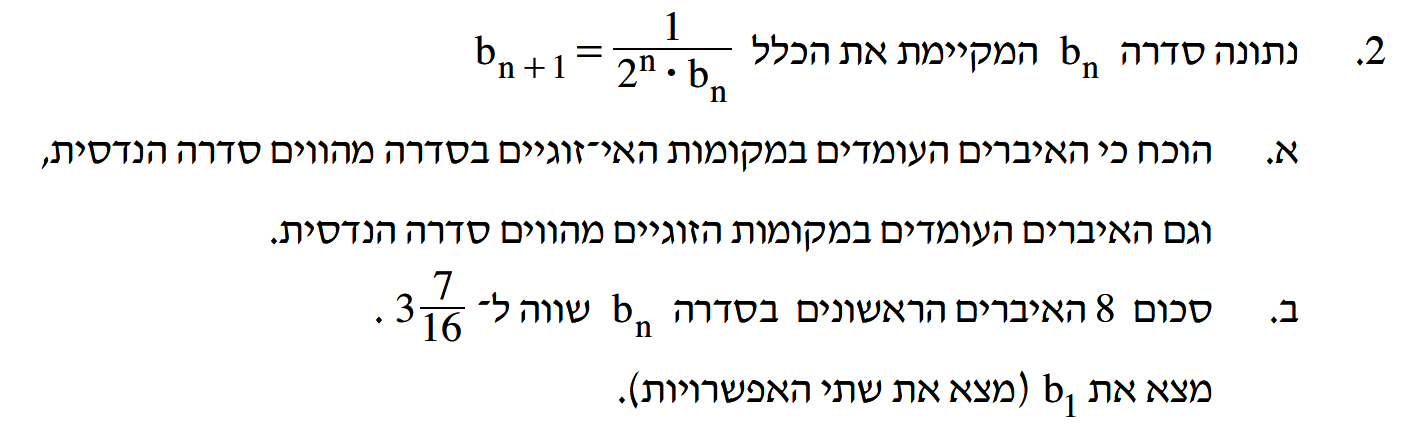
\includegraphics[width=.95\textwidth]{summer-2015b-2}
\end{center}
\vspace{-2ex}

\textbf{סעיף א}

החילוק של איברים במרחק שני מקומות אחד מהשני לא תלוי בזוגיות:
\[
\frac{b_{n+2}}{b_n} = \frac{1}{2^{n+1}b_{n+1}}\cdot\frac{1}{b_n}=\frac{1}{2^{n+1}\cdot\displaystyle\frac{1}{2^nb_n}{b_n}}= \frac{1}{2}\,.
\]
\textbf{סעיף ב}

 נחשב בנפרד את הסכום של ארבעת האיברים הזוגיים וארבעת האיברים האי-זוגיים:
\begin{eqnarray*}
S_{\mathit{odd}} &=& b_1+b_3+b_5+b_7=b_1\left(1 + \frac{1}{2} + \frac{1}{4} +\frac{1}{8}\right)=\frac{15}{8}b_1\\
S_{\mathit{even}} &=& b_2+b_4+b_6+b_8=b_2\left(1 + \frac{1}{2} + \frac{1}{4} +\frac{1}{8}\right)=\frac{15}{8}b_2=\frac{15}{8}\cdot\frac{1}{2^1b_1}\,.
\end{eqnarray*}
מ:
\[
S_{\mathit{odd}} + S_{\mathit{even}} =\frac{15}{8}\left(b_1+\frac{1}{2b_1}\right)= 3\frac{7}{16}=\frac{55}{16}\,.
\]
נקבל משוואה ריבועית 
$6b_1^2-11b_1+3=0$
שיש לה שני פתרונות 
$b_1=\frac{3}{2},\,\frac{1}{3}$.


%%%%%%%%%%%%%%%%%%%%%%%%%%%%%%%%%%%%%%%%%%%%%%%%%%%%%%%%%%%%%%%%%%%
\np

\section{חורף תשע"ו}

\begin{center}
\selectlanguage{english}
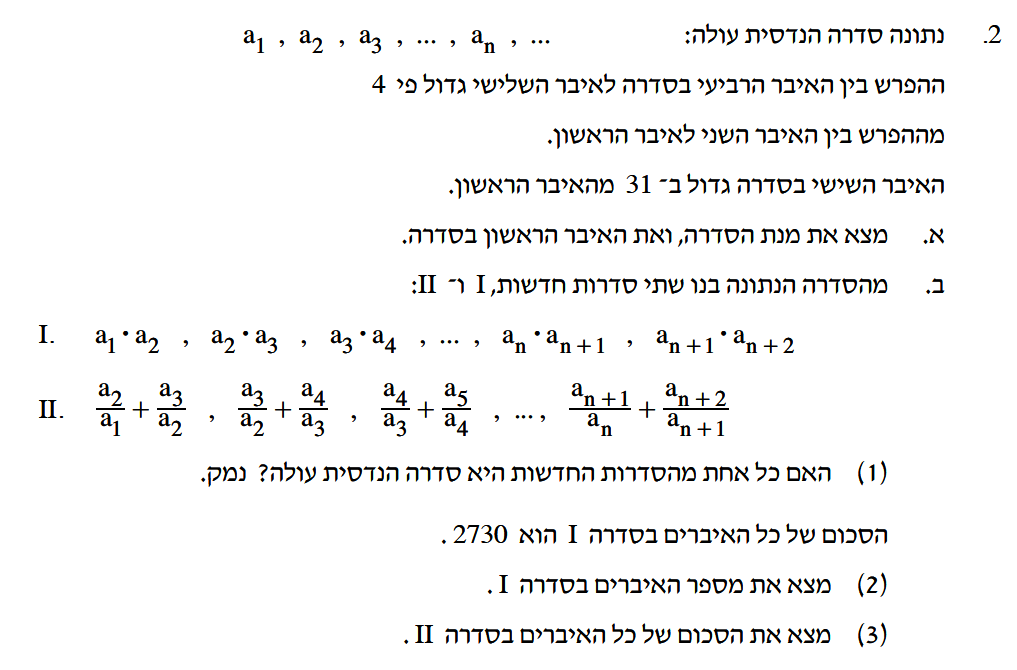
\includegraphics[width=.95\textwidth]{winter-2016-2}
\end{center}

\vspace{-4ex}

\textbf{סעיף א}

שימו לב ששואלים על
\textbf{ההפרשים}
של סדרה 
\textbf{הנדסית}.

המנתון הראשון:
\erh{2pt}
\begin{equationarray*}{rcl}
a_4-a_3 &=& 4 (a_2-a_1)\\
a_1q^3-a_1q^2 &=& 4(a_1q-a_1)\\
q^2(q-1)&=&4(q-1)\,.
\end{equationarray*}
\vspace{-5ex}

פתרון אחד של המשוואה הוא
$q=1$
אבל נתון שהסדרה עולה ולכן
$q\neq 1$.
אם 
$q\neq 1$,
נחלק ב-%
$q-1$
ונקבל
$q^2=4$.
כאשר המנה שלילי, הסימנים של איברי הסדרה מתחלפים, אז הפתרון היחיד הוא
$q=2$.

מהנתון השני:
\vspace{-2ex}
\erh{2pt}
\begin{equationarray*}{rcl}
a_6-a_1 &=& 31\\
a_1q^5-a_1&=& 31\\
32a_1-a_1&=&31\\
a_1&=&1\,.
\end{equationarray*}
\vspace{-6ex}

\textbf{סעיף ב} 
$(1)$

עבור סדרה I:
\[
q_I=\frac{a_{n+1}\cdot a_{n+2}}{a_n\cdot a_{n+1}}=\frac{a_{n+2}}{a_n}=\frac{a_n\,q^2}{a_n}=q^2=4\,,
\]
והסדרה היא סדרה הנדסית עולה.
\np

עבור סדרה II:
\[
q_{II}=\left(\frac{a_{n+1}}{a_n} + \frac{a_{n+2}}{a_{n+1}}\right) / \left(\frac{a_{n}}{a_{n-1}} + \frac{a_{n+1}}{a_{n}}\right)=\frac{q+q}{q+q}=1\,.
\]
הסדרה הנדסית אבל
\textbf{לא עולה}.

\smallskip

\textbf{סעיף ב}
$(2)$

מסכום הסדרה ניתן לחשב את מספר האיברים בסדרה:
\begin{eqnarray*}
a_1\cdot a_2 + \cdots + a_{n+1} \cdot a_{n+2} &=& 2730\\
(1\cdot 2)\cdot \frac{4^{n+1}-1}{4-1}&=&2730\\
4^{n+1}&=&4096\\
n&=&5\,.
\end{eqnarray*}
\begin{large}
\textbf{שימו לב!}
\end{large}
אמנם
$n=5$
אבל מספר האיברים בסדרה I הוא 
$n+1=6$:
\[
(1)\, a_1\cdot a_2,\;\; (2)\,a_2\cdot a_3,\;\;(3)\, a_3\cdot a_4,\;\; (4)\,a_4\cdot a_5,\;\; (5)\,a_5\cdot a_6,\;\; (6)\,a_6\cdot a_7 \;(= a_{n+1}\cdot a_{n+2})\,.
\]



\textbf{סעיף ב}
$(3)$

חישבנו
$q_{II}=1$.
נחשב את
$a_1^{II}$:
\[
a_1^{II}=\frac{a_{2}}{a_1} + \frac{a_{3}}{a_{2}}=\frac{2}{1}+\frac{4}{2}=4\,.
\]
\begin{large}
\textbf{שימו לב!}
\end{large}
מספר האיברים בסדרה II הוא 
$5$:
\[
(1)\,\frac{a_2}{a_1}+\frac{a_3}{a_2},\;\;
(2)\,\frac{a_3}{a_2}+\frac{a_4}{a_3},\;\;
(3)\,\frac{a_4}{a_3}+\frac{a_5}{a_4},\;\;
(4)\,\frac{a_5}{a_4}+\frac{a_6}{a_5},\;\;
(5)\,\frac{a_6}{a_5}+\frac{a_7}{a_6} \left(= \frac{a_{n+1}}{a_n}+\frac{a_{n+2}}{a_{n+1}}\right)\,.
\]

$q_{II}=1$
ולכן
\textbf{כל}
איברי הסדרה שווים ל-%
$a_1=4$.
הסכום הוא:
$4\cdot 5$.

%%%%%%%%%%%%%%%%%%%%%%%%%%%%%%%%%%%%%%%%%%%%%%%%%%%%%%%%%%%%%%%%%%%
\np
\section{קיץ תשע"ה מועד ב}

\begin{center}
\selectlanguage{english}
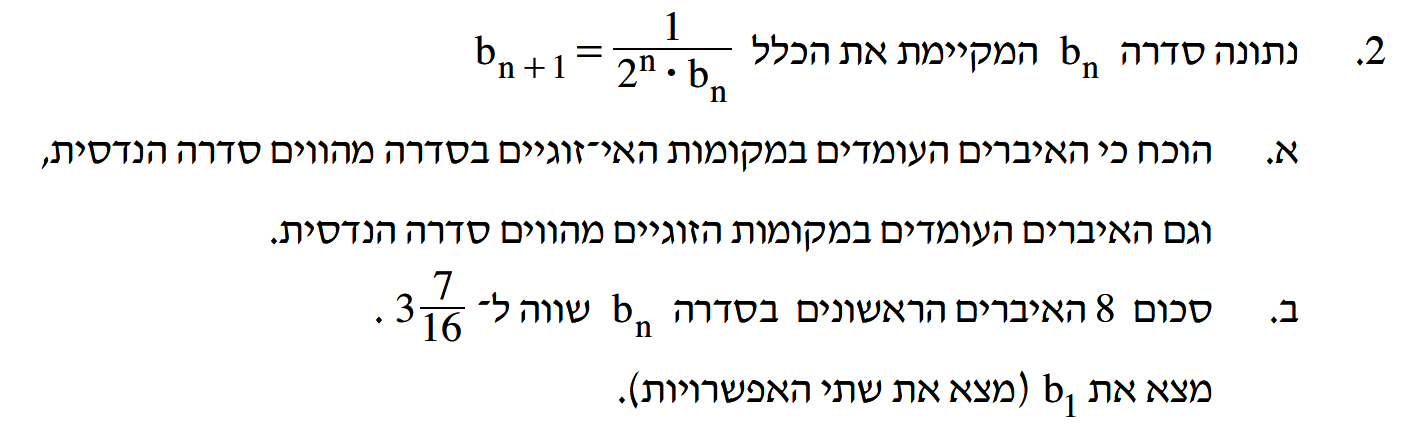
\includegraphics[width=.95\textwidth]{summer-2015b-2}
\end{center}
\vspace{-2ex}

\textbf{סעיף א}

החילוק של איברים במרחק שני מקומות אחד מהשני לא תלוי בזוגיות:
\[
\frac{b_{n+2}}{b_n} = \frac{1}{2^{n+1}\cdot b_{n+1}\cdot b_n}=\frac{1}{2^{n+1}\cdot\displaystyle\frac{1}{2^n\cdot b_n}\cdot {b_n}}= \frac{1}{2}\,.
\]
\textbf{סעיף ב}

אנחנו לא יודעים אם הסדרה כולה היא הנדסית, לכן נחשב בנפרד את הסכום 
של ארבעת האיברים הזוגיים וארבעת האיברים האי-זוגיים:
\erh{18pt}
\begin{equationarray*}{rcl}
S_{\mathit{odd}} &=& b_1+b_3+b_5+b_7=b_1\left(1 + \frac{1}{2} + \frac{1}{4} +\frac{1}{8}\right)=\frac{15}{8}b_1\\
S_{\mathit{even}} &=& b_2+b_4+b_6+b_8=b_2\left(1 + \frac{1}{2} + \frac{1}{4} +\frac{1}{8}\right)=\frac{15}{8}b_2=\frac{15}{8}\cdot\frac{1}{2^1b_1}\,.
\end{equationarray*}
מ:
\[
S_{\mathit{odd}} + S_{\mathit{even}} =\frac{15}{8}\left(b_1+\frac{1}{2b_1}\right)= 3\frac{7}{16}=\frac{55}{16}\,.
\]

נקבל משוואה ריבועית 
$6b_1^2-11b_1+3=0$
שיש לה שני פתרונות 
$\displaystyle b_1=\frac{3}{2},\,b_1=\frac{1}{3}$.

%%%%%%%%%%%%%%%%%%%%%%%%%%%%%%%%%%%%%%%%%%%%%%%%%%%%%%%%%%%%%%%%%%%
\np
\section{קיץ תשע"ה מועד א}

\begin{center}
\selectlanguage{english}
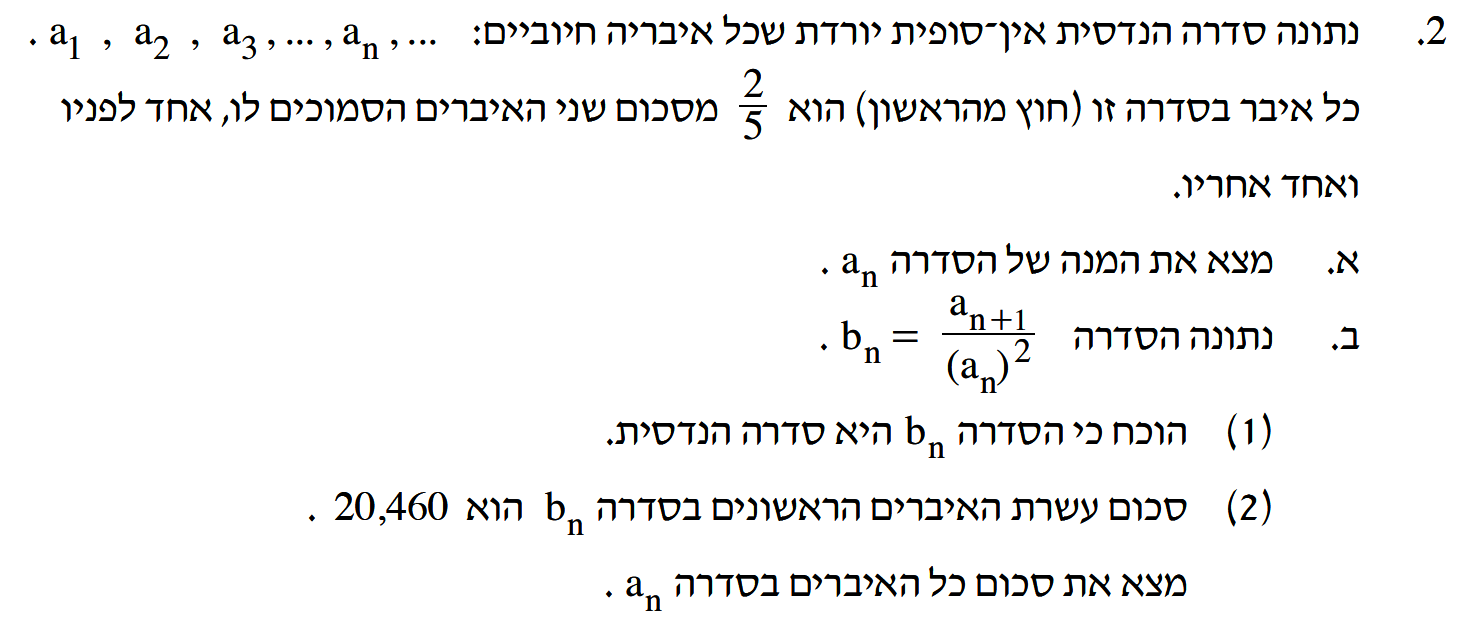
\includegraphics[width=.95\textwidth]{summer-2015a-2}
\end{center}
\vspace{-2ex}

\textbf{סעיף א}

נתון:
\[
a_n = \frac{2}{5}(a_{n-1}+a_{n+1}) =\frac{2}{5}\left(\frac{a_n}{q}+qa_n\right)
\]
עבור
$n\geq 2$.
$a_n$
מצטמצם ונקבל משוואה ריבועית
$2q^2-5q+2=0$
שיש לה שני פתורונות
$\displaystyle q=\frac{1}{2},	q=2$.
נתון שהסדרה יורדת ולכן
$\displaystyle q_a=\frac{1}{2}$.

\medskip

\textbf{סעיף ב}
$(1)$
\[
q_b=\frac{b_{n+1}}{b_n} = \frac{\displaystyle\frac{a_{n+2}}{(a_{n+1})^2}}{\displaystyle\frac{(a_{n})^2}{a_{n+1}}}= \frac{a_{n+2}}{(a_{n+1})^2}\cdot\frac{(a_{n})^2}{a_{n+1}} = \frac{a_nq^2}{(a_nq)^2}\cdot\frac{(a_n)^2}{a_nq}=\frac{1}{q}=2\,.
\]
\textbf{סעיף ב}
$(2)$

מ:
\[
S_{10}=\frac{b_1(2^{10}-1)}{2-1}=20460
\]
מתקבל
$b_1=20$.
השאלה מבקשת את סכום 
\textbf{הסדרה המקורית}
$a_{n}$.
כבר חישבנו את המנה
$q_a$
וניתן לחשב את
$a_1$
מהנוסחה עבור 
$b_n$:
\erh{16pt}
\begin{equationarray*}{rcl}
b_1 &=& \frac{a_2}{a_1^2} = \frac{a_1q_a}{(a_1)^2} = \frac{1}{2a_1}\\
a_1&=&\frac{1}{2b_1}=\frac{1}{40}\\
S_a &=& \frac{a_1}{1-q_a}=\frac{1}{40\left(1-\displaystyle\frac{1}{2}\right)} = \frac{1}{20}\,.
\end{equationarray*}

%%%%%%%%%%%%%%%%%%%%%%%%%%%%%%%%%%%%%%%%%%%%%%%%%%%%%%%%%%%%%%%%%%%

\np
\section{חורף תשע"ה}

\begin{center}
\selectlanguage{english}
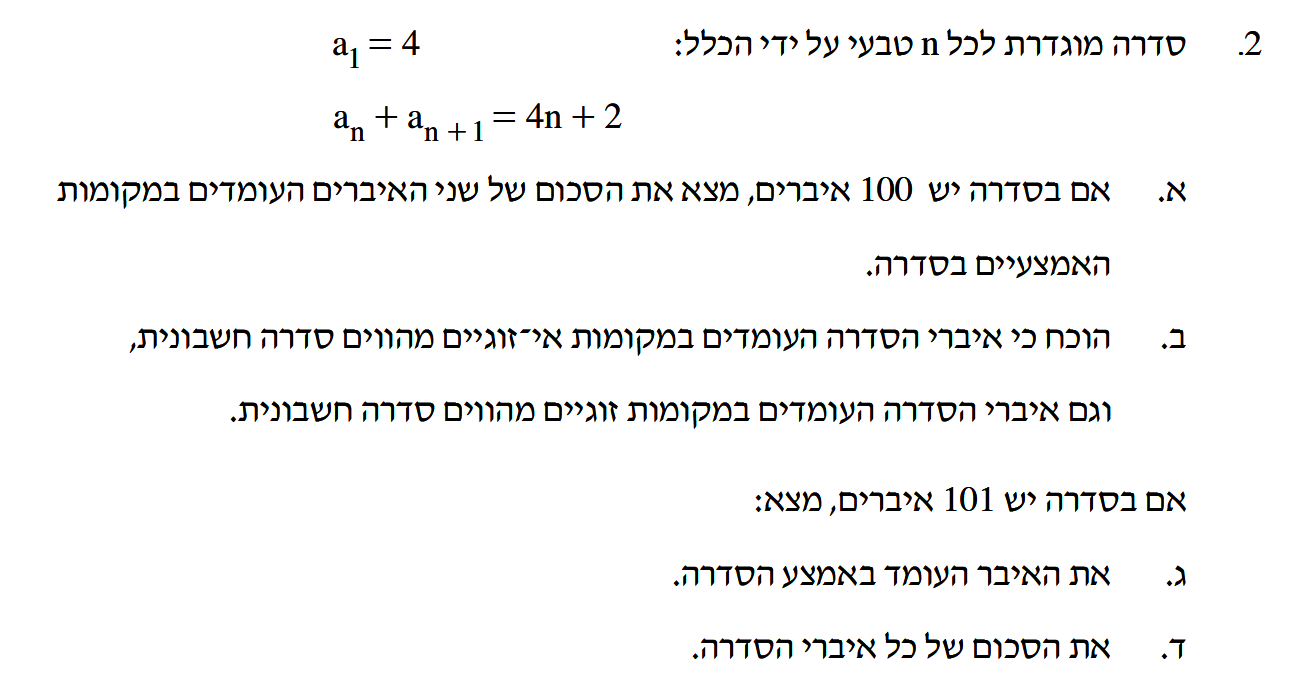
\includegraphics[width=.95\textwidth]{winter-2015-2}
\end{center}
\vspace{-1ex}

\textbf{שימו לב}
שלא נתון שהסדרה כולה היא חשבונית.

\textbf{סעיף א}

כדאי לרשום את איברי הסדרה כדי לוודא מהם האיברים האמצעיים:
\[
\overbrace{\rule{0pt}{8pt}a_1, a_2, \ldots, a_{49}, a_{50}}^{50}, \overbrace{\rule{0pt}{8pt}a_{51}, a_{52},\ldots, a_{100}}^{50}\,.
\]
ניתן לחשב את הסכום מהגדרת הסדרה:
\[
a_{50}+a_{51}=4\cdot 50+2=202\,.
\]
\textbf{סעיף ב}

במבט ראשון השאלה נראית בעייתית כי נתונה נוסחה לחישוב איברים סמוכים זה לזה
$a_n+a_{n+1}$,
אבל האיברים הזוגיים נמצאים במרחק שני מקומות זה מזה וכך גם האיברים האי-זוגיים
$a_{n+2}-a_{n}$.
חבל שאין לנו
$a_{n+1}-a_{n}$
ו-%
$a_{n+2}-a_{n+1}$.
צמד הביטויים האלה יכול לרמוז ל-"טריק" ידוע במתמטיקה: אם נוסיף ונחסיר את אותו ערך לביטוי, ערך הביטוי לא משתנה:
\begin{eqnarray*}
a_{k+2} - a_{k} &=& a_{k+2}+(a_{k+1}-a_{k+1})-a_{k}\\
&=& (a_{k+2}+a_{k+1})-(a_{k+1}+a_{k})\\
&=& (4(k+1)+2)-(4k+2)\\
&=&4\,.
\end{eqnarray*}
ההפרש קבוע ולא תלוי בזוגיות, ולכן הזוגיים והאי-זוגיים מהווים סדרות חשבוניות.

\np

\textbf{סעיף ג}

לא ידוע שהסדרה
$a_{n}$
חשבונית, אבל
$a_{51}$
הוא איבר בסדרת
\textbf{האי-זוגיים}.
נרשום את הסדרה כדי לדייק בספירת האיברים הזוגיים והאי-זוגיים:
\[
\overbrace{\rule{0pt}{8pt}a_1, a_2, \ldots, a_{49}, a_{50}}^{50}, a_{51}, \overbrace{\rule{0pt}{8pt}a_{52}, \ldots, a_{100}, a_{101}}^{50}\,.
\]
ברור שמספר האיברים האי-זוגיים גדול באחד ממספר האיברים הזוגיים,
$51$
אי-זוגיים ו-%
$50$
זוגיים. 
$a_{51}$
הוא האיבר ה-%
$25$
העומד באמצע הסדרה. האיבר הראשון של המספרים האי-זוגיים נתון,
$a_1=4$,
ואת ההפרש
$d=4$
חישבנו בסעיף הקודם. מכאן:
\[
a_{51}=a_1+25d =4+25\cdot 4=104\,.
\]

\textbf{סעיף ד}

נחשב את סכום הסדרה כחיבור של סכום האי-זוגיים וסכום הזוגיים.
$a_1=4$
נתון, וניתן לחשב לפי הנוסחה הנתונה:
\[
a_2=a_{1+1}=4\cdot 1+2-a_1=4+2-4=2\,.
\]
כבר חישבנו שהפרשים של שתי תת-הסדרות הם 
$4$.
מספר האי-זוגיים הוא
$51$
ומספר הזוגיים הוא
$50$.
הסכום הוא:
\[
S=S_{\mathit{odd}} + S_{\mathit{even}}=\frac{51}{2}(2\cdot 4+50\cdot 4)+\frac{50}{2}(2\cdot 2+49\cdot 4)=5304+5000=10304\,.
\]

%%%%%%%%%%%%%%%%%%%%%%%%%%%%%%%%%%%%%%%%%%%%%%%%%%%%%%%%%%%%%%%%%%%
\np

\section{קיץ תשע"ד מועד ב}

\begin{center}
\selectlanguage{english}
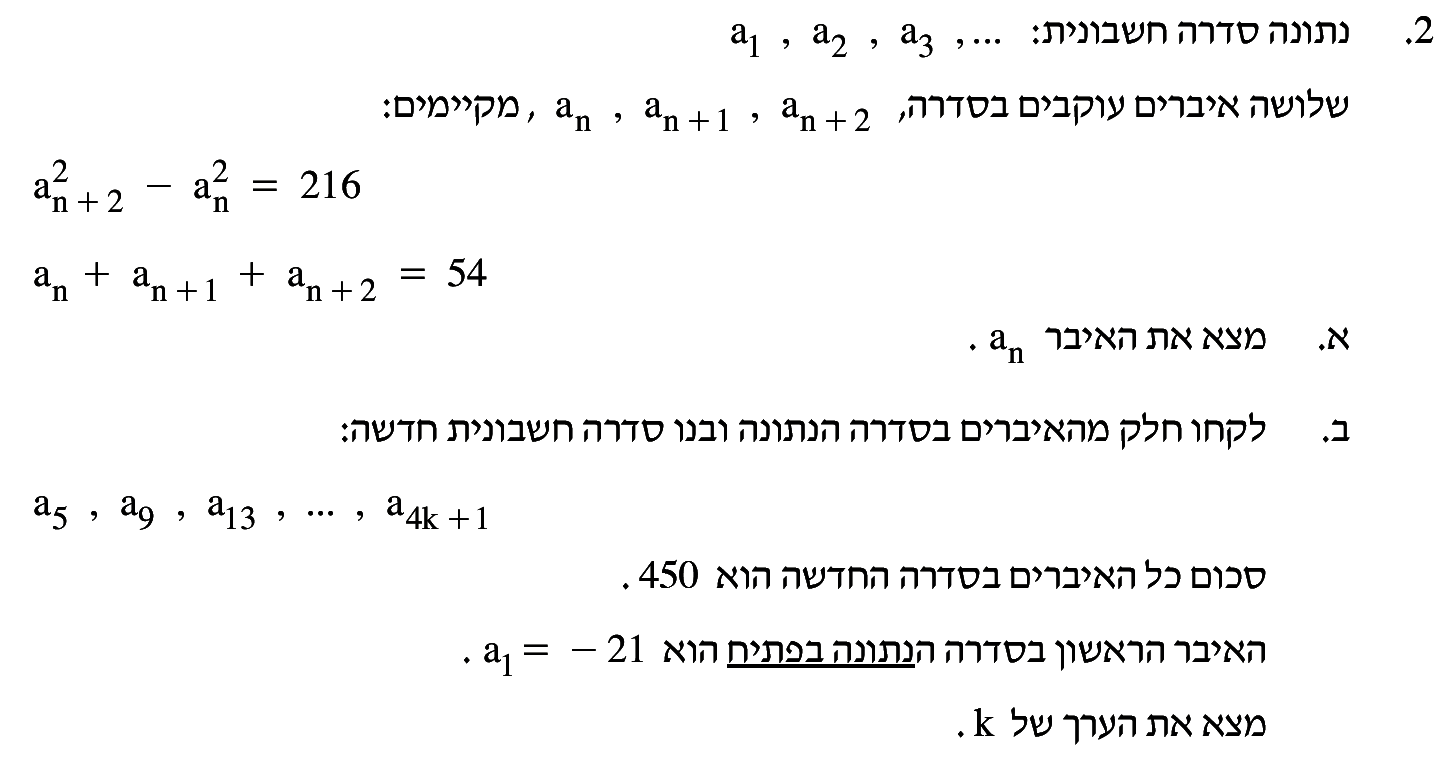
\includegraphics[width=.95\textwidth]{summer-2014b-2}
\end{center}
\vspace{-2ex}


\textbf{סעיף א}

הסדרה חשבונית ולכן ניתן להשתמש להציב בתוך המשוואות הנתונות ולקבל שתי משוואות עם שני נעלמים:
\erh{4pt}
\begin{equationarray*}{rcl}
(a_n+2d)^2 - a_n^2 &=& 216\\
4a_nd+4d^2 &=& 216\\
a_n+(a_n+d)+(a_n+2d)&=&54\\
3a_n + 3d &=& 54\,.
\end{equationarray*}
הפתרון הוא
$d=3,a_n=15$.

\smallskip

\textbf{סעיף ב}

הסדרה החדשה חשבונית שאיבריה 
$a'_1, a'_2,\ldots$
הם:
\[
\overbrace{a_5=a_1+4d}^{a_1'}, \quad a_6=a_5+5d,\quad  a_7=a_5+6d,\quad  a_8=a_5+7d,\quad  \overbrace{a_9=a_5+8d}^{a_2'}\,.
\]
בסדרה החדשה
$d' = 4d = 12$
ו-%
$a_1' = a_5 = -21 + 4d= -9$.
מסכום הסדרה החדשה:
\[
\frac{k}{2}(2a'_1 + (k-1)d')=\frac{k}{2}(-18+(k-1)\cdot 12)=450
\]
מתקבלת משוואה ריבועית
$2k^2-5k-150=0$
שהשורש החיובי שלה הוא
$k=10$.


%%%%%%%%%%%%%%%%%%%%%%%%%%%%%%%%%%%%%%%%%%%%%%%%%%%%%%%%%%%%%%%%%%%

\np
\section{קיץ תשע"ד מועד א}

\begin{center}
\selectlanguage{english}
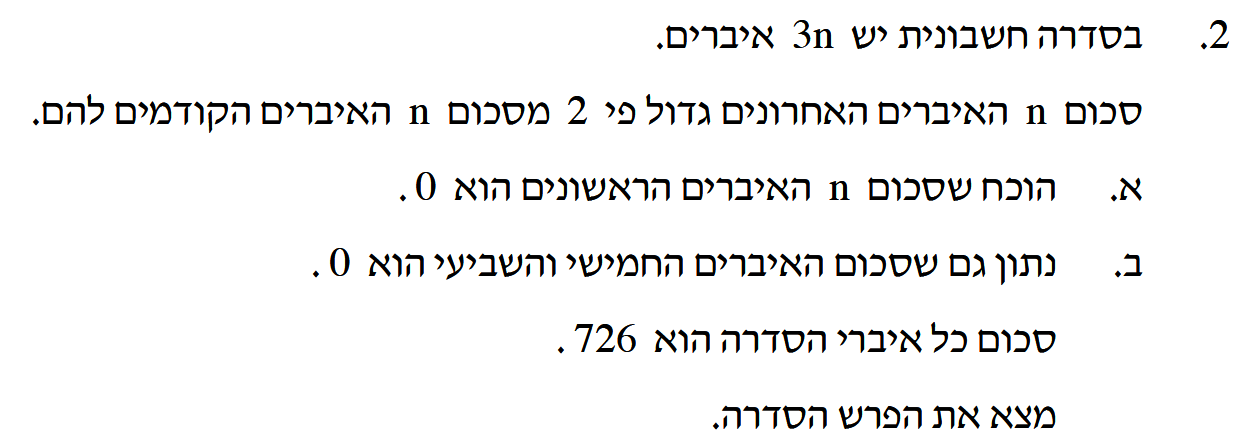
\includegraphics[width=.9\textwidth]{summer-2014a-2}
\end{center}

\vspace{-4ex}

\textbf{סעיף א}

כדי לדייק עם האינדקסים כדאי לרשום את הסדרה עם סימון של הסדרות החלקיות:
\[
\underbrace{
\overbrace{\rule{0pt}{8pt}a_1, a_2, \ldots, a_n}^{S_1},
\overbrace{\rule{0pt}{8pt}a_{n+1}, a_{n+2}, \ldots, a_{2n}}^{S_2},
\overbrace{\rule{0pt}{8pt}a_{2n+1}, a_{2n+2}, \ldots, a_{3n}}^{S_3}
}_{S_{3n}}\,.
\]
נתון
$S_3=2S_2$:
\[
\erh{10pt}
\begin{array}{lll}
\displaystyle\frac{n}{2}(2(a_1+2nd)+(n-1)d)&=&2\cdot \displaystyle\frac{n}{2}(2(a_1+nd)+(n-1)d)\\
2a_1+(5n-1)d&=&4a_1+(6n-2)d\\
2a_1+(n-1)d&=&0\,.
\end{array}
\]
הביטוי בצד השמאלי של המשוואה האחרונה הוא הסכום 
$S_1$.

דרך אחרת לפתור את הבעיה היא להחסיר את סכום התת-הסדרות מסכום הסדרה כולה:
\erh{14pt}
\begin{equationarray*}{rcl}
S_1&=& S_{3n} - (S_2+S_3) =  S_{3n} - (S_2 + 2S_2) = S_{3n} - 3S_2\\
&=&\displaystyle\frac{3n}{2}(2a_1+(3n-1)d) -3\cdot\displaystyle \frac{n}{2}(2(a_1+nd)+(n-1)d)\\
&=&0\,.
\end{equationarray*}

\np

\begin{center}
\fbox{
\begin{minipage}{.8\textwidth}
בבחינה של חורף תשע"ב אורך הסדרה הוא
$2n-1$,
ונתונים הסכומים של
$n$
האיברים הראשונים ו-%
$n$
האיברים האחרונים. רק רישום זהיר של הסדרה יבהיר שיש חפיפה בין שתי תת-הסדרות:
\[
\renewcommand{\arraystretch}{.3}
\begin{array}{ll}
\overbrace{\rule{0pt}{8pt}a_1, a_2, \ldots, a_n}^{n},&\hspace{-9pt}a_{n+1}, a_{n+2}, \ldots, a_{2n-1}\,.\\
&\hspace{-2em}\underbrace{\rule{10em}{0pt}}_{n}
\end{array}
\]
בדוגמה קל יותר לשים לב לחפיפה. עם
$n=4$:
\[
\renewcommand{\arraystretch}{.3}
\begin{array}{ll}
\overbrace{\rule{0pt}{8pt}a_1, a_2, a_3, a_4}^{4},&\hspace{-9pt}a_5, a_6, a_7\,.\\
&\hspace{-2em}\underbrace{\rule{5em}{0pt}}_{4}
\end{array}
\]
\vspace*{-1ex}
\end{minipage}
}
\end{center}

\bigskip

\textbf{סעיף ב}

נתון סכום הסדרה ועלינו למצוא
$d$
למרות שאין לנו 
$a_1$.
נבדוק אם הנתון השני יכול לעזור:
\[
a_5+a_7=(a_1 + 4d) + (a_1 + 6d) = 0\,.
\]
מכאן ש-%
$a_1=-5d$.


בסעיף א חישבנו ש-%
$S_1=0$
ונציב עבור 
$a_1$:
\[
\frac{n}{2}(-10d+(n-1)d)=0\,.
\]
$d$
לא יכול להיות
$0$
כי אחרת מהנתון שהסכום של שני איברים הוא אפס אפשר להסיק שכל איברי הסדרה הם אפס. זה סותר את הנתון שהסכום הוא מספר חיובי. לכן אפשר לחלק את המשוואה ב-%
$d$
ונקבל
$n=11$.

נציב עבור
$a_1,n$
בנוסחה ל-%
$S_{3n}$:
\erh{16pt}
\begin{equationarray*}{rcl}
S_3&=&\frac{3n}{2}(2a_1+(3n-1)d)\\
&=&\frac{33}{2}(-10d+(33-1)d)\\
&=&\frac{33}{2}\cdot 22d = 363d=726\,,
\end{equationarray*}
ונקבל 
$d=2$.

%%%%%%%%%%%%%%%%%%%%%%%%%%%%%%%%%%%%%%%%%%%%%%%%%%%%%%%%%%%%%%%%%%%
\np

\section{חורף תשע"ד}

\begin{center}
\selectlanguage{english}
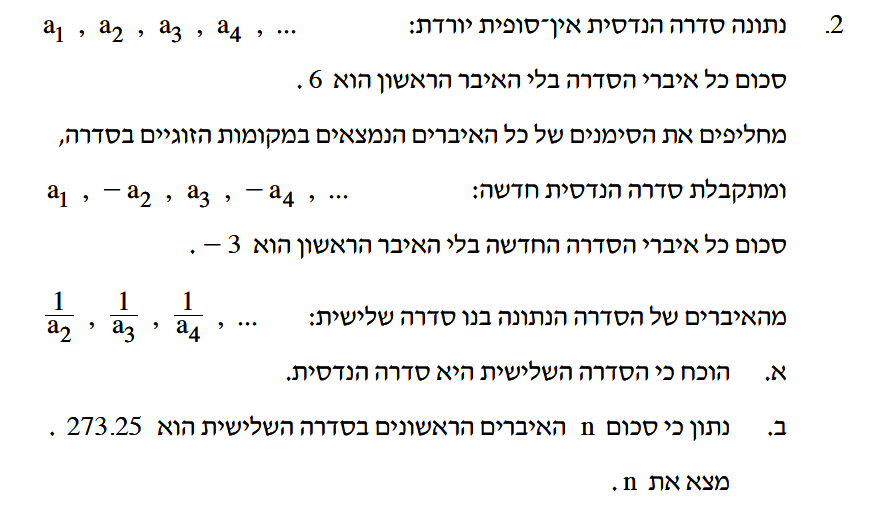
\includegraphics[width=.9\textwidth]{winter-2014-2}
\end{center}
\vspace{-2ex}
\textbf{סעיף א}

המנה של הסדרה השלישית קבועה כי נתון שהסדרה הראשונה הנדסית:
\[
\frac{1/a_{n+1}}{1/a_n}=\frac{a_n}{a_{n+1}}\,.
\]
\textbf{סעיף ב}

נשתמש בשני הסכומים הנתונים כדי לכתוב שתי משוואות עם שני נעלמים:
\erh{12pt}
\begin{equationarray*}{rcl}
\frac{a_2}{1-q}&=&6\\
\frac{-a_2}{1-(-q)}&=& -3\,.
\end{equationarray*}
הפתרון הוא 
$q=\displaystyle\frac{1}{3}$
ו-%
$a_2=4$.

בסדרה השלישית, האיבר הראשון הוא 
$\displaystyle \frac{1}{a_2}=\frac{1}{4}$
וההפרש הוא
$\displaystyle \frac{1}{d}=3$
מהסכום השלישי ונקבל:
\erh{12pt}
\begin{equationarray*}{rcl}
\frac{1}{4}\cdot \frac{3^n-1}{3-1}&=&273.25\\
3^n&=&2187\\
n&=&7\,,
\end{equationarray*}
כאשר בדקנו חזקות של
$3$
עד שהתקבל
$2187$.



%%%%%%%%%%%%%%%%%%%%%%%%%%%%%%%%%%%%%%%%%%%%%%%%%%%%%%%%%%%%%%%%%%%

\np
\section{המלצות}

\begin{itemize}


\item
\textbf{חובה לקרוא את השאלות בזהירות רבה.}
בבחינה של קיץ תשע"ה א, סעיף ב שואלת על סדרה חדשה
${b_n}$
אבל בסוף חוזרת ומבקשת למצוא את הסכום של הסדרה הנתונה
${a_n}$.

\item
שימו לב אם סדרה היא חשבונית, הנדסית או לא זו ולא זו.

\item 
ברוב השאלות נתונה סדרה ומוגדרת סדרה חדשה המובססת על הסדרה הנתונה. 
\textbf{אין בהכרח קשר}
בין תכונה של הסדרה המקורית והסדרה החדשה. להלן שתי סדרות חשבוניות, אבל כאשר משלבים את שתיהן, מתקבלת סדרה שאיננה חשבונית:
\[
\begin{array}{rrrrrrrrrrr}
1,& 4,& 7,& 10,& 13,& \ldots\\
2,& 5,& 8,& 11,& 14, &\ldots\\
1,& 2,& 4,& 5,& 7,& 8,& 10,& 11,& 13,& 14, &\ldots
\end{array}
\]
\item
כאשר מבקשים להוכיח שתת-סדרת הזוגיים חשבונית או הנדסית וגם תת-סדרת האי-זוגיים, הוכחה אחת תספיק כי אם 
$\displaystyle \frac{a_{n+2}}{a_n}$
קבוע, לא משנה אם 
$n$
זוגי או אי-זוגי.


\item
כדאי לרשום את איברי הסדרה כדי לדייק במקומות של האיברים:
\[
\setlength{\extrarowheight}{8pt}
\begin{array}{l}
\overbrace{\rule{0pt}{8pt}a_1, a_2, \ldots, a_{49}, a_{50}}^{50}, \overbrace{\rule{0pt}{8pt}a_{51}, a_{52},\ldots, a_{100}}^{50}\\
\underbrace{\rule{0pt}{8pt}a_1, a_2, \ldots, a_{49}, a_{50}}_{50}, a_{51}, \underbrace{\rule{0pt}{8pt}a_{52}, \ldots, a_{100}, a_{101}}_{50}\,.
\end{array}
\]
\vspace{-3ex}

\item
מקרה מעניין הוא תת-סדרות חופפות )בחינה של חורף תשע"ב שלא נמצאת במסמך זה(:
\[
\renewcommand{\arraystretch}{.4}
\begin{array}{ll}
\overbrace{\rule{0pt}{8pt}a_1, a_2, \ldots, a_n}^{n},&\hspace{-9pt}a_{n+1}, a_{n+2}, \ldots, a_{2n-1}\\
&\hspace{-2em}\underbrace{\rule{10em}{0pt}}_{n}
\end{array}
\]
\vspace{-4ex}
\item
קיימות שתי דרכים לסכם מספר תת-סדרות )בחינה של קיץ תשע"ד א(. דרך אחת היא לסכם כל תת-סדרות בנפרד עם ערכי ה-%
$d, a_1$
או
$n, q$
שלהן. זה קורה לעתים קרובות כאשר השאלה מבקשת לחשב סכום של סדרה, אבל ידוע רק שתת-סדרות חשבוניות או הנדסיות, למשל, זוגיים ואי-זוגיים )בחינה של קיץ תשע"ח ב(.
\item 
דרך אחרת היא לחבר הסכומים של תת-סדרות ולהחסיר את התוצאה מסכום הסדרה כולה:
\[
S_1 = S_n - (S_2+S_3)\,.
\]
\vspace{-6ex}

\item
בסדרה קיימים ארבעה נעלמים
$d, a_1$
או
$S, n, q$.
כדי למצוא את ערכו של נעלם אחד, צריך לדעת את ערכי שלושת הנעלמים האחרים )או שניים אם לא מדובר בסכום(. לפעמים, מספיק לדעת את הקשר בין שני נעלמים, כגון
$a_1+11d = 0$
בבחינה של הורף תשע"ח.

\np

\item
הבחינה של חורף תשע"ו מעניינת כי מספר האיברים הוא לא הערך של המספר 
$n$
המופיע בשאלה. חשוב לרשום דוגמה מספרית כדי לוודא מהו מספר האיברים:
\[
(1)\, a_1\cdot a_2,\;\; (2)\,a_2\cdot a_3,\;\;\cdots\;\; (5)\,a_5\cdot a_6=(a_n\cdot a_{n+1}),\;\; (6)\,a_6\cdot a_7 \;(= a_{n+1}\cdot a_{n+2})\,.
\]
\vspace{-4ex}

\item
טריק שימושי הוא לחבר ולהחסיר את אותו ערך בביטוי )בחינה  חורף תשע"ה(:
\[
a_{k+2} - a_{k} = a_{k+2}+(a_{k+1}-a_{k+1})-a_{k} = (a_{k+2}+a_{k+1})-(a_{k+1}+a_{k})\,.
\]
\vspace{-4ex}

\item
הכנסת איברים חדשים בתוך סדרה לא בהכרח שומרת על הסדרה כחשבונית או הנדסית. השורה הראשונה להלן היא סדרה חשבונית. בשורה השנייה הוכנסו איברים של סדרה חשבונית נוספת והסדרה החדשה היא חשבונית. בשורה השלישית הוכנסו איברים של סדרה חשבונית נוספת והסדרה החדשה איננה חשבונית.
\[
\begin{array}{rrrrrrrrrrrrr}
1,& 5,& 9,& 13,& 17\\
1, &3,& 5,&7,& 9,& 11,& 13, &15, & 17\\
1, &2,& 5,&6,& 9,& 10,& 13, &14, & 17
\end{array}
\]
בבחינה של קיץ תשע"ו ב כתוב במפורש שהסדרה חדשה חשבונית.

\item
בhישוב הפרש או מנה, כדאי להציב ב-%
$a_{n+1}$
או
$a_{n-1}$
ביטוי שיש בו 
$a_n$.
הנה דוגמה מהבחינה של  קיץ תשע"ה א:
\[
a_n = \frac{2}{5}(a_{n-1}+a_{n+1}) =\frac{2}{5}\left(\frac{a_n}{q}+qa_n\right)\,.
\]
$a_n$
מצטמצם ונקבל משוואה ריבועית ב-%
$q$.

\end{itemize}

\selectlanguage{english}

\tikzsetfigurename{probability}
% !TeX root = chapter1.tex

\chapter{הסתברות}



במסמך זה נפתור את השאלות על הסתברות בבחינות הבגרות, שאלון
$806$.
מצאתי שהבעיות עצמן קלות יחסית, בתנאי שמבינים את ניסוחי השאלות ואיך לתרגם אותן לחישובים המתאימים. בסוף המסמך סיכמתי את הניסוחים שמופיעים בשאלות.


%%%%%%%%%%%%%%%%%%%%%%%%%%%%%%%%%%%%%%%%%%%%%%%%%%%%%%%%%%%%%%%%%%%


\textbf{\R{
חורף תשע"ח
}}

\begin{center}
\selectlanguage{english}
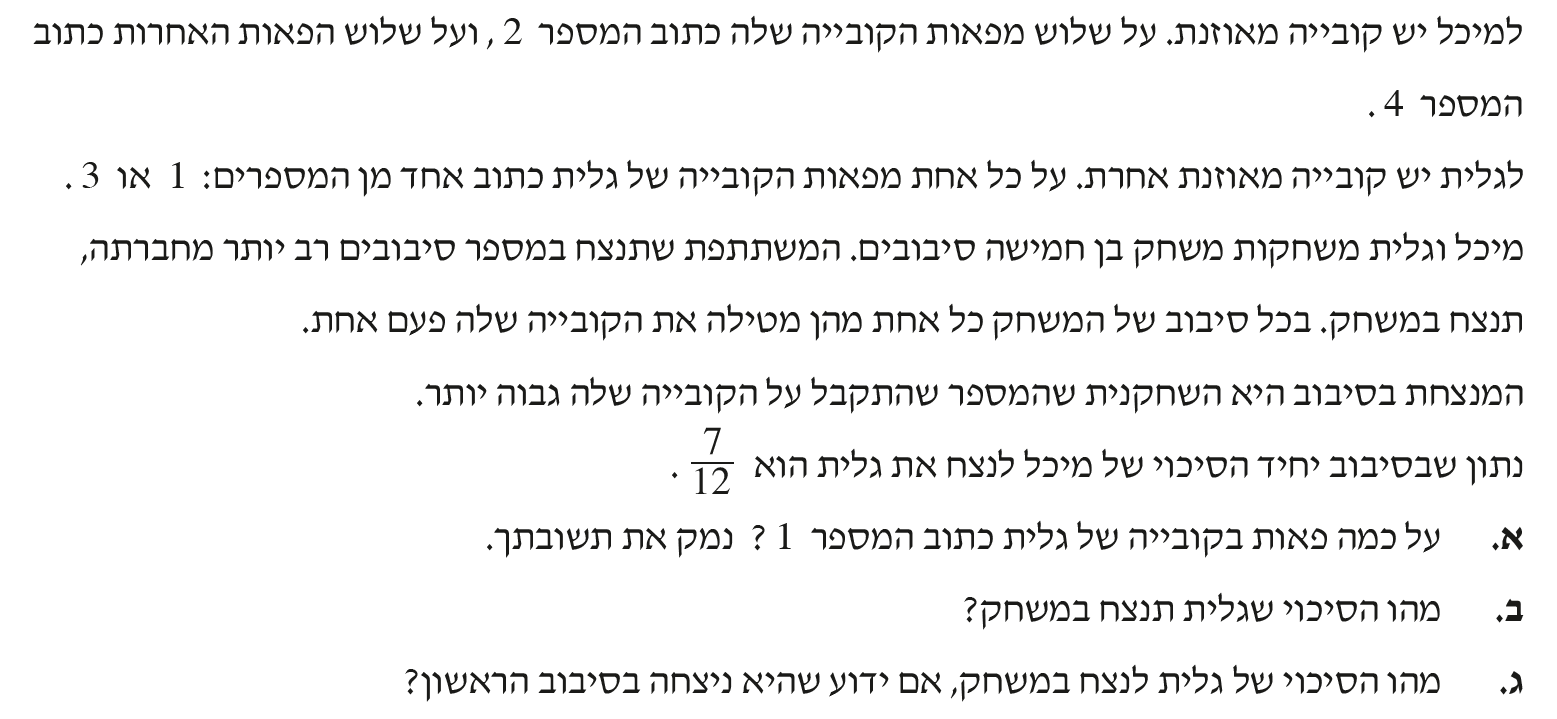
\includegraphics[width=\textwidth]{winter-2018-3}
\end{center}

סעיף א. מיכל תנצח אם )א( היא מטילה 
$4$
לא משנה מה גלית מטילה, אירוע שההסתברות שלה היא 
$1$,
או )ב( מיכל מטילה 
$2$
וגלית מטילה
$1$,
אירוע שההסתברות שלה היא
$\frac{n}{6}$,
כאשר נסמן ב-%
$n$
את המספר הפאות של הקוביה של גלית שכתוב עליהן
$1$.
המשוואה לניצחון של מיכל היא:
\[
\frac{3}{6}\cdot 1 + \frac{3}{6}\cdot \frac{n}{6}=\frac{7}{12}\,,
\]
והפתרון הוא
$n=1$.

סעיף ב. גלית תנצח במשחק אם היא תנצח ב-%
$3,4,5$
סיבובים:
\[
{5\choose 3}\left(\frac{5}{12}\right)^3\left(\frac{7}{12}\right)^2+{5\choose 4}\left(\frac{5}{12}\right)^4\left(\frac{7}{12}\right)^1+{5\choose 5}\left(\frac{5}{12}\right)^5\left(\frac{7}{12}\right)^0=0.3466\,.
\]
סעיף ג. המילים 
\textbf{אם ידוע}
מכוונות להסתברות מותנית:
\vspace{-4ex}
\[
\renewcommand{\arraystretch}{2.4}
\begin{array}{c}
P(\textrm{\R{גלית תנצח}}/\textrm{\R{גלית ניצחה בסיבוב הראשון}}) =\\
\displaystyle\frac{P(\textrm{\R{גלית תנצח}}\cap\textrm{\R{גלית ניצחה בסיבוב הראשון}})}{P(\textrm{\R{גלית ניצחה בסיבוב הראשון}})}\,.
\end{array}
\]
ההסתברות במנה: כדי שגלית תנצח במשחק וגם בסיבוב הראשון, היא חייבת לנצח בסיבוב הראשון וגם ב-%
$2,3,4$
מהסיבובים הנותרים:
\[
\frac{5}{12}\left[{4 \choose 4}\left(\frac{5}{12}\right)^4 \left(\frac{7}{12}\right)^0+
{4 \choose 3}\left(\frac{5}{12}\right)^3 \left(\frac{7}{12}\right)^1+
{4 \choose 2}\left(\frac{5}{12}\right)^2 \left(\frac{7}{12}\right)^2\right]
=\frac{5}{12}\cdot 0.5534\,.
\]
ההסתברות במכנה היא כמובן 
$\frac{5}{12}$,
ולכן התשובה היא
$0.5534$.

%%%%%%%%%%%%%%%%%%%%%%%%%%%%%%%%%%%%%%%%%%%%%%%%%%%%%%%%%%%%%%%%%%%
\newpage

\textbf{\R{
קיץ תשע"ח, מועד א
}}

\begin{center}
\selectlanguage{english}
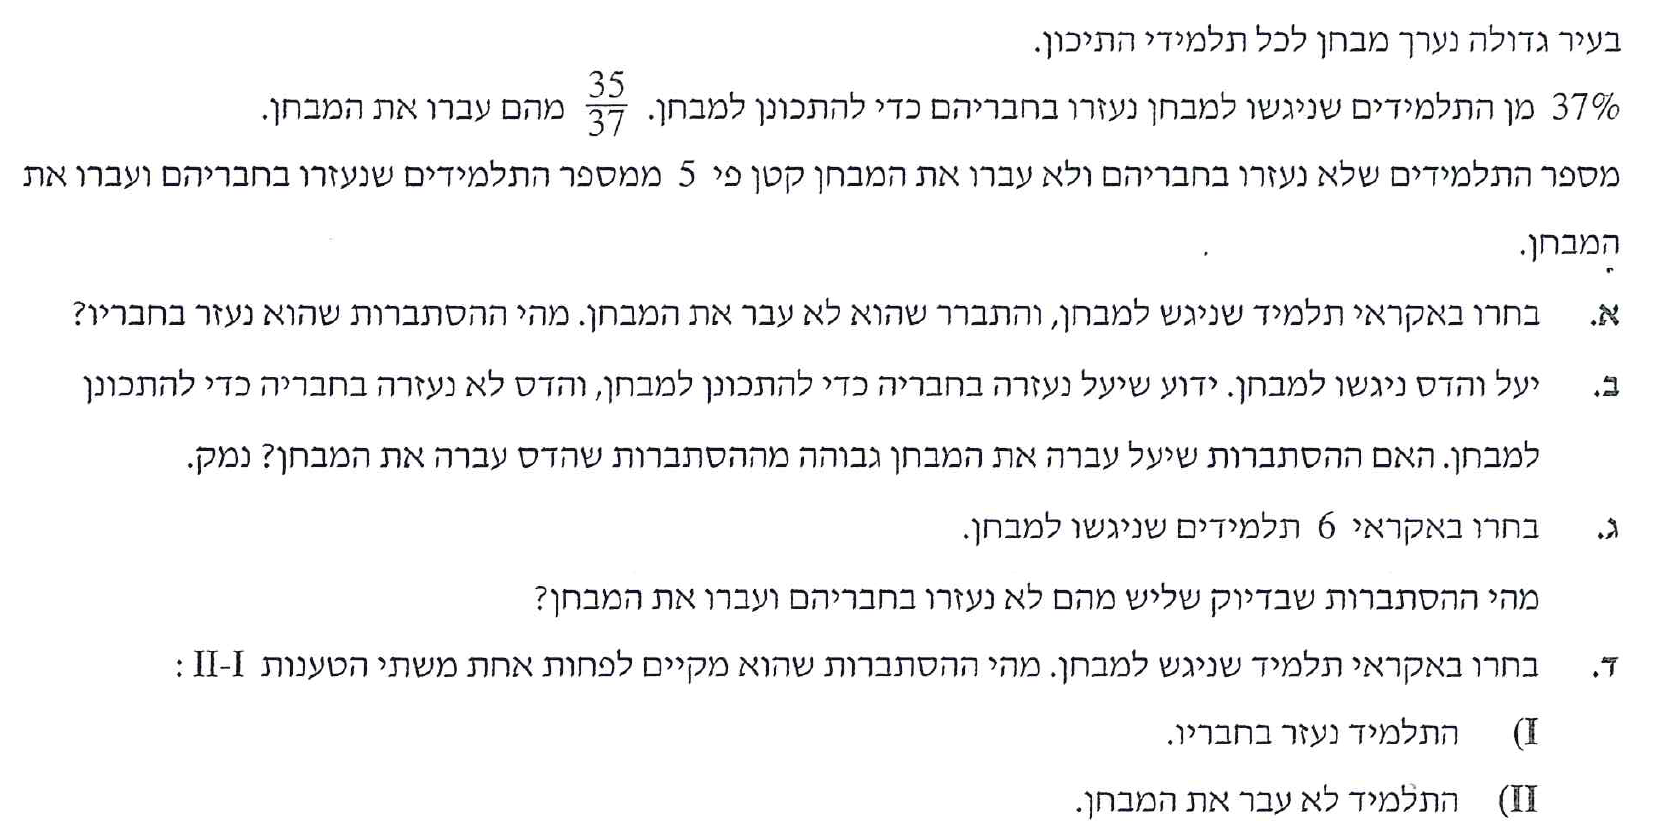
\includegraphics[width=	\textwidth]{summer-2018a-3}
\end{center}
נסמן ב-%
$N$
את התלמידים שנעזרו בחבריהם, וב-%
$A$
את התלמידים שעברו את המבחן. נתון ש-%
$P(N)=0.37$.
\textbf{מהם}
עברו את הבחינה 
$\displaystyle\frac{35}{37}$,
ההסתברות המותנית
$P(A/N)$.
נחשב:
\[
P(A/N) = \frac{P(N\cap A)}{P(N)} = \frac{P(N\cap A)}{0.37}=\frac{35}{37},\quad\quad\quad P(N\cap A)=0.35\,.
\]
עד כאן טבלת ההסתברויות היא:
\begin{center}
\selectlanguage{english}
\begin{tikzpicture}[scale=1.25]
\draw (0,0) grid (3,3);
\node at (2.5,3.3) {$\bm{A}$};
\node at (1.5,3.3) {$\bover{A}$};
\node at (3.3,2.5) {$\bm{N}$};
\node at (3.3,1.5) {$\bover{N}$};
\node at (2.5,2.5) {$0.35$};
\node at (0.5,2.5) {$0.37$};
\node at (1.5,2.5) {$0.02$};
\node at (0.5,1.5) {$0.63$};
\node at (0.5,0.5) {$1.0$};
\end{tikzpicture}
\end{center}
בהמשך נתון ש-%
\[
P(\overline{N}\cap\overline{A})=\frac{P(N\cap A)}{5}=\frac{0.35}{5}=0.07\,,
\]
וניתן להשלים את הטבלה:
\begin{center}
\selectlanguage{english}
\begin{tikzpicture}[scale=1.25]
\draw (0,0) grid (3,3);
\node at (2.5,3.3) {$\bm{A}$};
\node at (1.5,3.3) {$\bover{A}$};
\node at (3.3,2.5) {$\bm{N}$};
\node at (3.3,1.5) {$\bover{N}$};
\node at (2.5,2.5) {$0.35$};
\node at (0.5,2.5) {$0.37$};
\node at (1.5,2.5) {$0.02$};
\node at (0.5,1.5) {$0.63$};
\node at (0.5,0.5) {$1.0$};
\node at (1.5,0.5) {$0.09$};
\node at (2.5,0.5) {$0.91$};
\node at (1.5,1.5) {$0.07$};
\node at (2.5,1.5) {$0.56$};
\end{tikzpicture}
\end{center}
סעיף א.
\[
P(N/\overline{A})=\frac{P(N\cap \overline{A})}{P(\overline{A})}=\frac{0.02}{0.09}=\frac{2}{9}\,.
\]
סעיף ב. עבור יעל:
\[
P(A/N)=\frac{P(A \cap N)}{P(N)}=\frac{0.35}{0.37}=0.9459\,,
\]
ועבור הדס:
\[
P(A/\overline{N})=\frac{P(A\cap \overline{N})}{P(\overline{N})}=\frac{0.56}{0.63}=0.8889\,.
\]
ליעל הסתברות גבוהה יותר לעבור את המבחן.

סעיף ג. שליש של שש הוא שניים. )שימו לב שלא לקרוא "שלושה" במקום "שליש"!( החישוב הוא לפי נוסחת ברנולי כאשר הערך של
$P(\overline{N}\cap A)$
נמצא בטבלה:
\[
{6 \choose 2}(0.56)^2 (1-0.56)^4=0.1763\,.
\]
סעיף ד. הניסוח "%
\textbf{לפחות אחת}
משתי הטענות
$I, II$"
אומר שהאירוע קורה אם קורה אחד מהאירועים
$I, II$
\textbf{או שניהם}.
באיור להלן שני עגולים המייצגים את שני האירועים
$I, II$.
האירוע "לפחות אחד משניהם" מיוצג על ידי כל השטח המקווקו.
\begin{center}
\selectlanguage{english}
\begin{tikzpicture}
\begin{scope}
\clip[draw] (0,0) circle[radius=2];
\foreach \y in {-1.5,-1,-.5,0,.5,1,1.5}
  \draw (-2,\y) -- (2,\y);
\end{scope}
\begin{scope}
\clip[draw] (2.5,0) circle[radius=2];
\foreach \x in {1,1.5,2,2.5,3,3.5,4}
  \draw (\x,-2) -- (\x,2);
\end{scope}
\node at (-2,2.5) {$I$};
\node at (4.5,2.5) {$II$};
\node at (1.25,2.5) {$I\cap II$};
\node at (-3.5,.2) {$I-II$};
\node at (6,.2) {$II-I$};
\draw[->] (1.25,2.2) -- ++(0,-1);
\draw[->] (-3,.2) -- ++(1.7,0);
\draw[->] (5.5,.2) -- ++(-1.7,0);
\draw[->] (-2,2.2) -- +(.6,-.6);
\draw[->] (4.5,2.2) -- +(-.6,-.6);
\end{tikzpicture}
\end{center}
יש שתי דרכים לחשב את ההסתברות. בדרך הראשונה אנו לוקחים את סכום ההסתברויות של שני האירועים, וחסירים את ההסתברות של האירוע המשותף כי ספרנו אותו פעמיים, פעם כחלק מהאירוע 
$I$
ופעם כחלק מהאירוע
$II$:
\[
P(I \cup II) = P(I) + P(II) - P(I \cap II)\,.
\]
בדרך השניה אנו סופרים כל חלק מהאירוע השותף בנפרד, כאשר הסימון
$A-B$
הוא כל האיברים בקבוצה 
$A$
שאינם בקבוצה
$B$:
\[
P(I \cup II) = P(I-II) + P(II-I) + P(I \cap II)\,.
\]
את ההסתברויות לחישוב ניקח מהטבלה. הדרך הראשונה מופיעה מימין והדרך השניה משמאל:
\begin{center}
\selectlanguage{english}
\begin{tikzpicture}[scale=1.25]
\begin{scope}
\draw (0,0) grid (3,3);
\node at (2.5,3.3) {$\bm{A}$};
\node at (1.5,3.3) {$\bover{A}$};
\node at (3.3,2.5) {$\bm{N}$};
\node at (3.3,1.5) {$\bover{N}$};
\node at (2.5,2.5) {$0.35$};
\node at (0.5,2.5) {$0.37$};
\node at (1.5,2.5) {$0.02$};
\node at (0.5,1.5) {$0.63$};
\node at (0.5,0.5) {$1.0$};
\node at (1.5,0.5) {$0.09$};
\node at (2.5,0.5) {$0.91$};
\node at (1.5,1.5) {$0.07$};
\node at (2.5,1.5) {$0.56$};
\draw[ultra thick] (2,2) rectangle +(1,1);
\draw[ultra thick] (1,1) rectangle +(1,1);
\draw[ultra thick] (1,2) rectangle +(1,1);
\end{scope}
\begin{scope}[xshift=6cm]
\draw (0,0) grid (3,3);
\node at (2.5,3.3) {$\bm{A}$};
\node at (1.5,3.3) {$\bover{A}$};
\node at (3.3,2.5) {$\bm{N}$};
\node at (3.3,1.5) {$\bover{N}$};
\node at (2.5,2.5) {$0.35$};
\node at (0.5,2.5) {$0.37$};
\node at (1.5,2.5) {$0.02$};
\node at (0.5,1.5) {$0.63$};
\node at (0.5,0.5) {$1.0$};
\node at (1.5,0.5) {$0.09$};
\node at (2.5,0.5) {$0.91$};
\node at (1.5,1.5) {$0.07$};
\node at (2.5,1.5) {$0.56$};
\draw[ultra thick] (0,2) rectangle +(1,1);
\draw[ultra thick] (1,0) rectangle +(1,1);
\draw[ultra thick] (1,2) rectangle +(1,1);
\end{scope}
\end{tikzpicture}
\end{center}
בשתי הדרכים מקבלים אותה תוצאה:
\[
\renewcommand{\arraystretch}{1.5}
\begin{array}{l}
P(N\cup\overline{A})=P(N) + P(\overline{A}) - P(N\cap\overline{A}) = 0.37+0.09-0.02=0.44\\
P(N\cup\overline{A})=P(N-\overline{A}) + P(\overline{A}-N) + P(N\cap\overline{A}) = 0.35+0.07+0.02=0.44\,.
\end{array}
\]


%%%%%%%%%%%%%%%%%%%%%%%%%%%%%%%%%%%%%%%%%%%%%%%%%%%%%%%%%%%%%%%%%%%

\textbf{\R{
קיץ תשע"ח, מועד ב
}}

\begin{center}
\selectlanguage{english}
%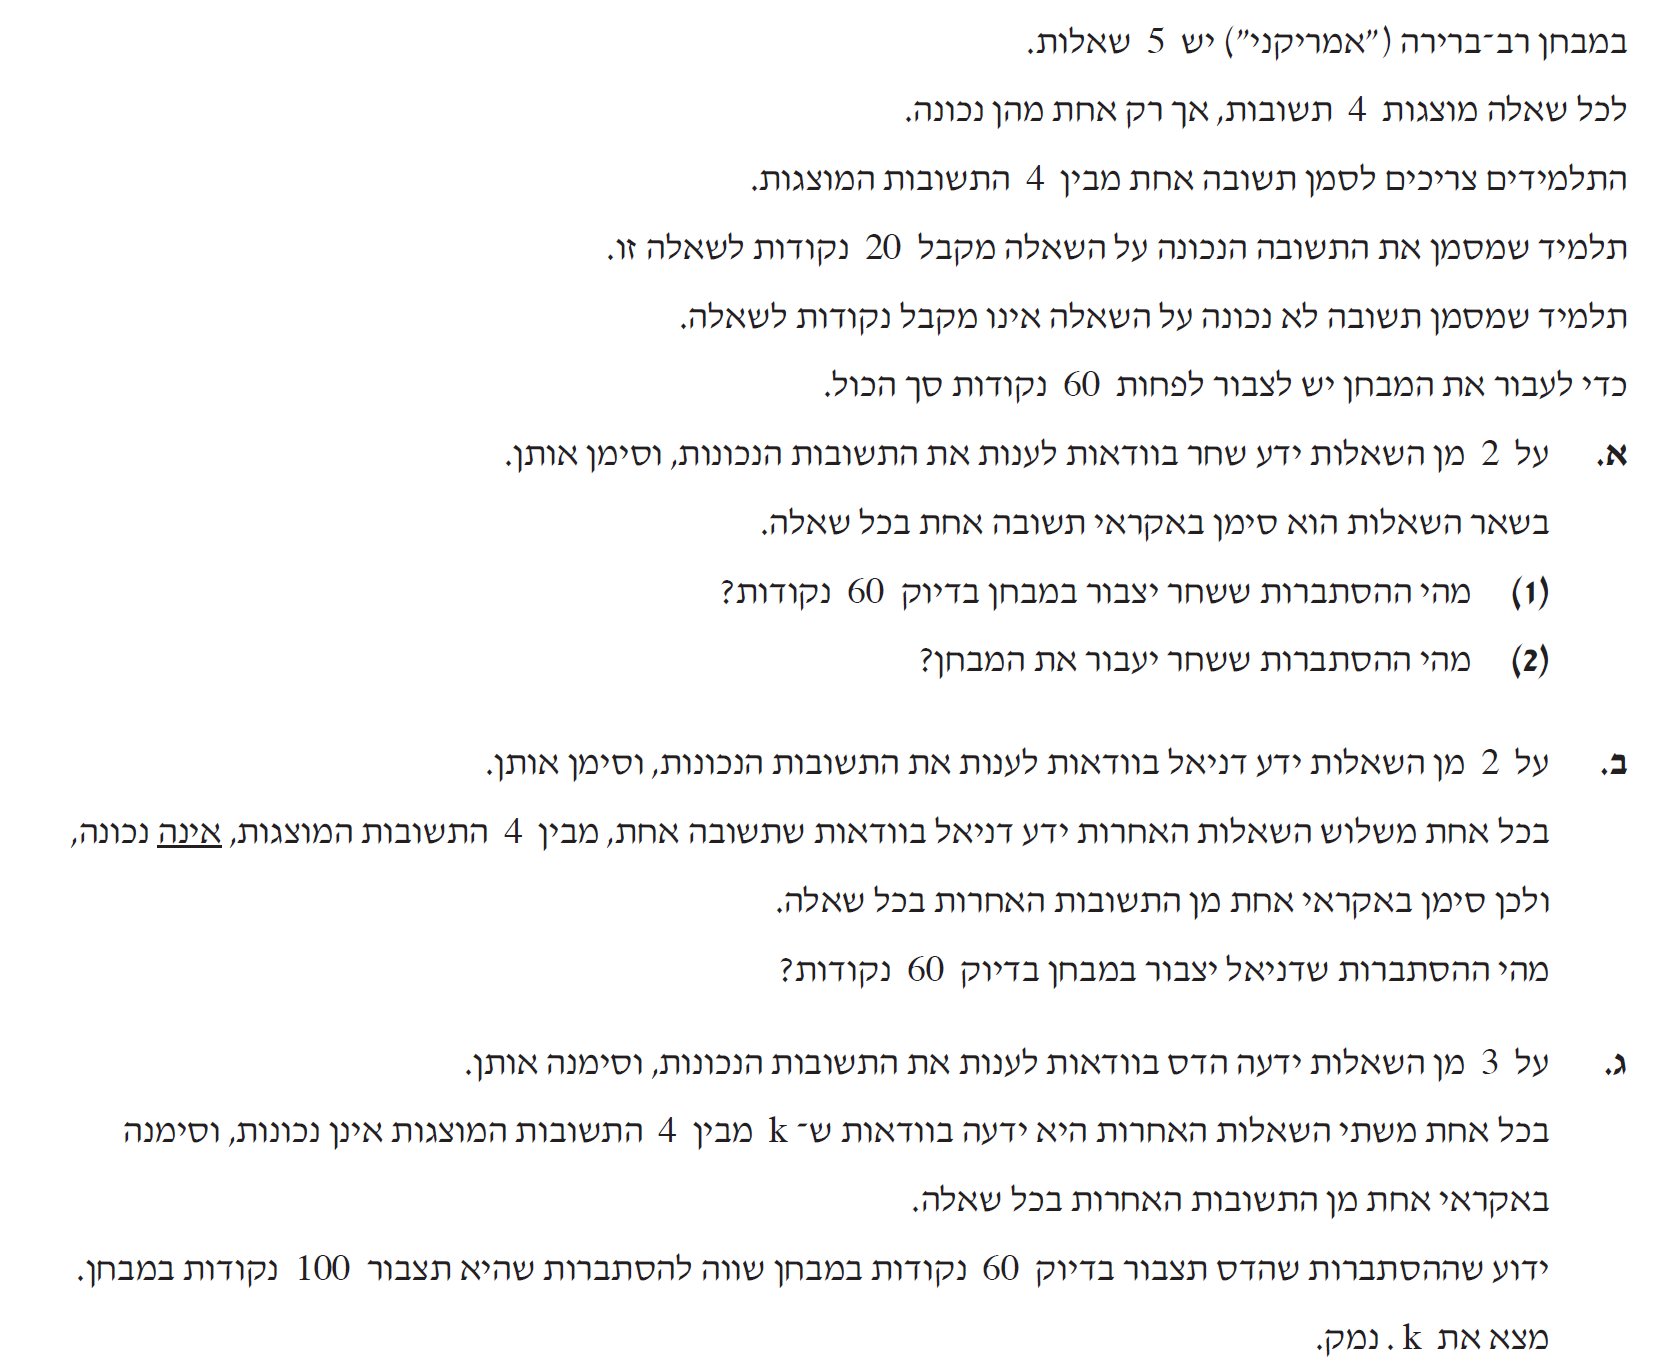
\includegraphics[width=\textwidth]{summer-2018b-3}
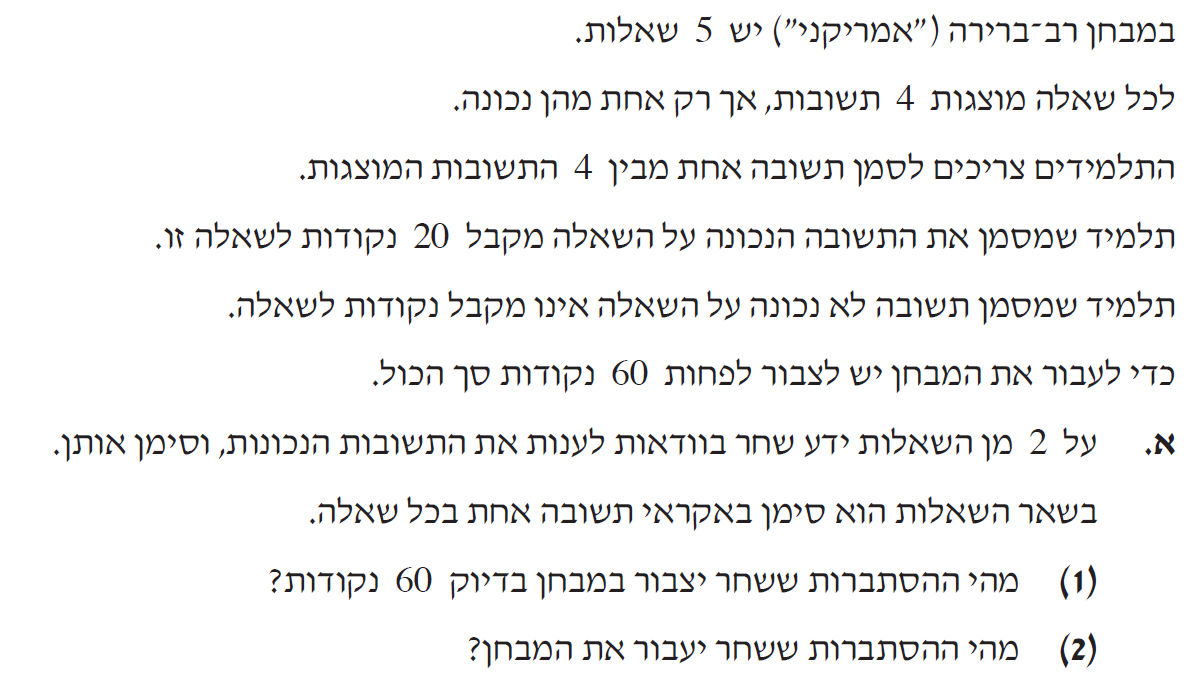
\includegraphics[width=.85\textwidth]{summer-2018b-3-1}
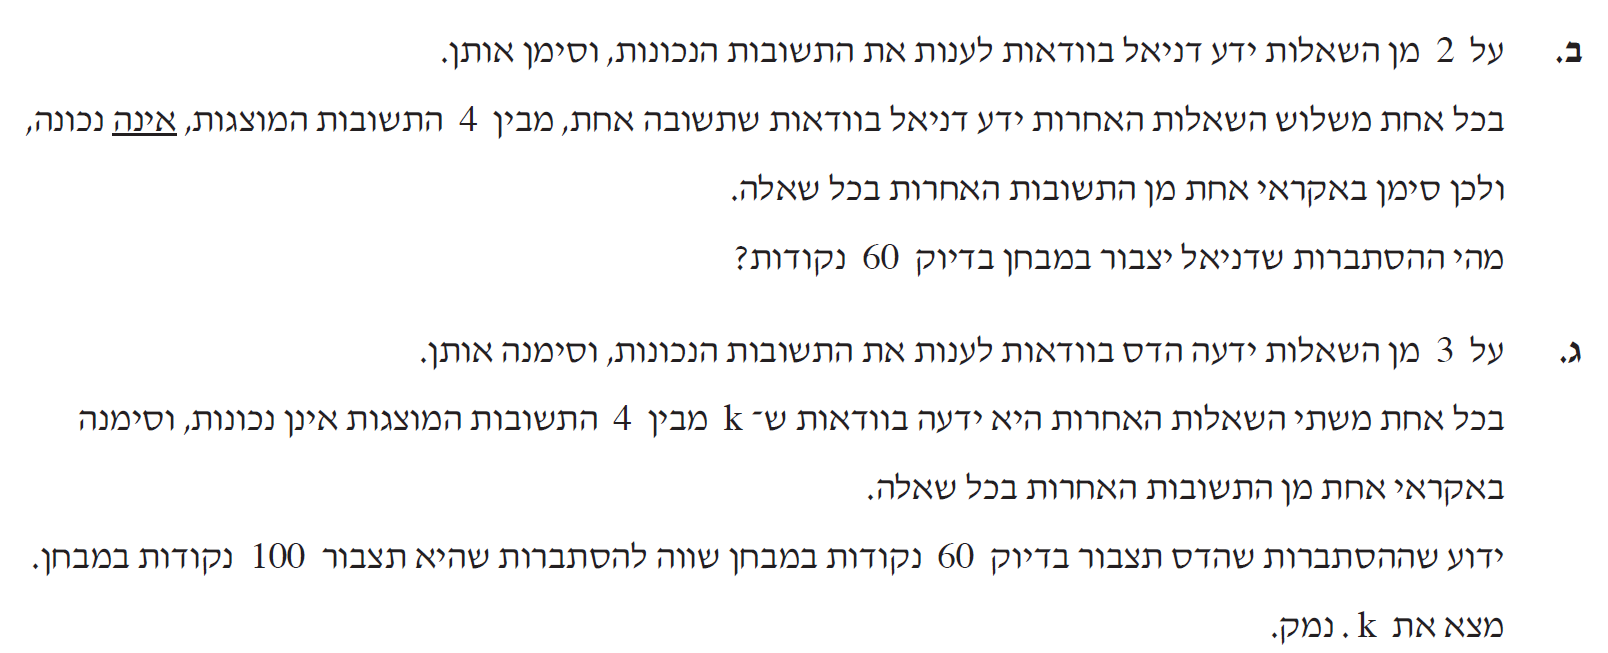
\includegraphics[width=\textwidth]{summer-2018b-3-2}
\end{center}

סעיף א
$(1)$.
שחר ידע שהוא ענה נכון על שתי שאלות ולכן כדי לקבל ציון
$60$
עליו לענות על 
\textbf{בדיוק אחת}
משלושת השאלות האחרות:
\[
{3 \choose 1}\left(\frac{1}{4}\right)\left(\frac{3}{4}\right)^2=\frac{27}{64}\,.
\]
סעיף א
$(2)$.
כדי לעבור את המבחן עליו לצבור
\textbf{לפחות}
שלוש תשובות נכונות. יש להוסיף את ההסבתרויות של ארבע וחמש תשובות נכונות:
\[
\frac{27}{64}+{3 \choose 2}\left(\frac{1}{4}\right)^2\left(\frac{3}{4}\right)^1+{3 \choose 3}\left(\frac{1}{4}\right)^3\left(\frac{3}{4}\right)^0=\frac{37}{64}\,.
\]
סעיף ב.
דניאל צירך לענות נכון על שאלה אחת 
\textbf{בדיוק}
מתוך שלושת השאלות הנותרות. דניאל ידע שתשובה אחת מתוך ארבע לא נכונה, לכן ההסתברות שהוא ענה נכון על השאלה היא
$\frac{1}{3}$:
\[
{3 \choose 1}\left(\frac{1}{3}\right)\left(\frac{2}{3}\right)^2=\frac{4}{9}\,.
\]
סעיף ג. אם הדס ידעה ש-%
$k$
מתוך 
$4$
תשובות לא נכונות, ההסתברות שהיא ענתה תשובה נכונה היא
$\frac{1}{4-k}$,
וההסתברות שהיא תענה תשובה לא נכונה היא
$\frac{4-k-1}{4-k}$.
כדי לקבל ציון 
\textbf{בדיוק}
$100$
הדס צריכה לבחור תשובות נכונות לשתי השאלות הנותרות. כדי לקבל ציון 
\textbf{בדיוק}
$60$
עליה לבחר תשובות לא נכונות לשתי השאלות הנותרות.

אין צורך להשתמש בנוסחת ברנולי במלואו, כי כאשר מחשבים את ההסתברות של "כל" או "אף אחד", 
${n\choose k}=1$,
וגם
$(1-p)^0=1$
או
$p^0=1$.
לכן, מספיק לחשב את ההסתברות של האירוע לחזקת מספר השאלות:
\begin{eqnarray*}
\left(\frac{1}{4-k}\right)^2 &=&\left(\frac{4-k-1}{4-k}\right)^2\\
(3-k)^2&=&1\\
k^2-6k+8&=& 0\,.
\end{eqnarray*}
הפתרונות הם 
$k=2,4$
אבל נתון ש-"אחת ]מהתשובות[ נכונה", לכן הפתרון היחיד הוא
$k=2$.

%%%%%%%%%%%%%%%%%%%%%%%%%%%%%%%%%%%%%%%%%%%%%%%%%%%%%%%%%%%%%%%%%%%

\newpage

\textbf{\R{
חורף תשע"ז
}}

\begin{center}
\selectlanguage{english}
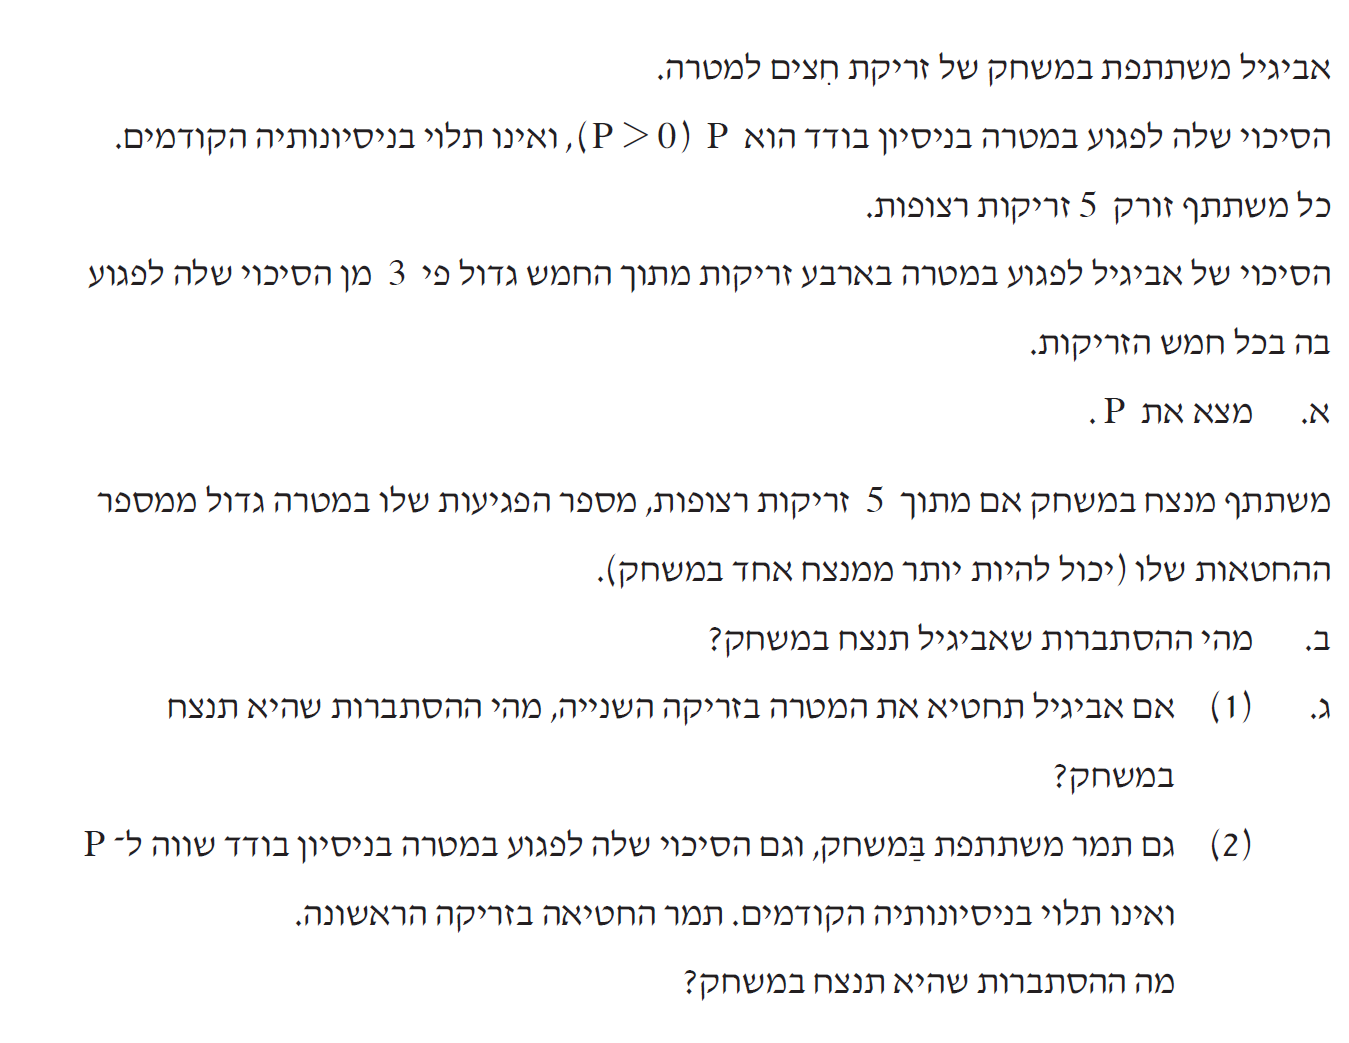
\includegraphics[width=.95\textwidth]{winter-2017-3.png}
\end{center}
\vspace{-1ex}

סעיף א. לפי המידע הנתון:
\[
{5 \choose 4} p^4(1-p)^1 = 3{5\choose 5}p^5(1-p)^0\,.
\]
והפתרון הוא
$p=\frac{5}{8}$.

סעיף ב. ההסתברות ל-%
$3,4,5$
פגיעות היא:
\[
{5 \choose 3}p^3(1-p)^2 + {5 \choose 4}p^4(1-p)^1 + {5 \choose 5}p^5(1-p)^0
\]
נציב
$p=\frac{5}{8}$
ונקבל
$0.7248$.

סעיף ג 
$(1)$.
לדעתי, ניסוח השאלה לא ברור. אני פירשתי אותה: מה ההסתברות של
\textbf{האירוע}
"אביגיל מחטיאה בזריקה השנייה ופוגעת בשלוש או ארבע מהזריקות האחרות"? כותב הבחינה התכוון להסתברות מותנית: "%
\textbf{אם ידוע ש-}%
אביגיל החטיאה בזריקה השנייה, מה ההסתברות שהיא פוגעת בשלוש או ארבע מהזריקות האחרות"?
\[
\renewcommand{\arraystretch}{2}
\begin{array}{c}
P(1,3,4,5\ \textrm{\R{אביגיל פגעה בשלוש או ארבע מהזריקות}}/\textrm{\R{אביגיל החטיאה בזריקה השניה}}) =\\
\displaystyle\frac{P(1,3,4,5\ \textrm{\R{אביגיל פגעה בשלוש או ארבע מהזריקות}}\cap \textrm{\R{אביגיל החטיאה בזריקה השניה}})}{P(\textrm{\R{אביגיל החטיאה בזריקה השניה}})}\,.
\end{array}
\]
אפשר לפתור את הבעיה בשתי דרכים. נתחיל עם הדרך הפשוטה יותר. נתון שהסיכוי לפגוע במטרה אינו תלוי בניסיונות הקודמים, ולכן ההסתברויות בלתי תלויות והחישוב מצטמצם:
\[
\renewcommand{\arraystretch}{2}
\begin{array}{c}
\displaystyle\frac{P(1,3,4,5\ \textrm{\R{אביגיל פגעה בשלוש או ארבע מהזריקות}}) \cdot P(\textrm{\R{אביגיל החטיאה בזריקה השניה}})}{P(\textrm{\R{אביגיל החטיאה בזריקה השניה}})}=\\
P(1,3,4,5\ \textrm{\R{אביגיל פגעה בשלוש או ארבע מהזריקות}})\,.
\end{array}
\]
החישוב הוא:
\[
{4\choose 4}\left(\frac{5}{8}\right)^4 \left(\frac{3}{6}\right)^0 +{4\choose 3}\left(\frac{5}{8}\right)^3\left(\frac{3}{8}\right)^1 = 0.5188\,.
\]
הדרך השנייה ארוכה יותר אבל מעניינת. האירוע של החיתוך בנוסחה להסתברות מותנית מורכבת משני אירועים: )א( לא משנה מה יצאה מהזריקה הראשונה, הזריקה השניה החטיאה, ושלושת הזריקות האחרונות פגעו. )ב( הזריקה הראשונה פגעה, הזריקה השניה החטיאה, ושתיים מתוך שלושת הזריקות האחרונות פגעו. הסתברות של האירוע המשותף היא:
\[
1\cdot \frac{3}{8} \cdot \left(\frac{5}{8}\right)^3 \quad + \quad
\frac{5}{8}\cdot \frac{3}{8} \cdot \left[{3\choose 2}\left(\frac{5}{8}\right)^2\frac{3}{8}\right] = 0.1945\,.
\]
נחלק ב-%
$\frac{3}{8}$,
ההסתברות האביגיל החטיאה בזריקה השנייה, ונקבל 
$0.5188$.

סעיף ג 
$(2)$.
לא משנה איזו זריקה החטיאה, הזריקות בלתי תלויות וחישוב ההסתברות של "תמר פגעה בשלוש  או ארבע מהזריקות 
$2,3,4,5$"
נותן אותה תוצאה כמו האירוע "אביגיל פגעה בשלוש או ארבע מהזריקות 
$1,3,4,5$".

%%%%%%%%%%%%%%%%%%%%%%%%%%%%%%%%%%%%%%%%%%%%%%%%%%%%%%%%%%%%%%%%%%%
\bigskip

\textbf{\R{
קיץ תשע"ז, מועד א
}}

\begin{center}
\selectlanguage{english}
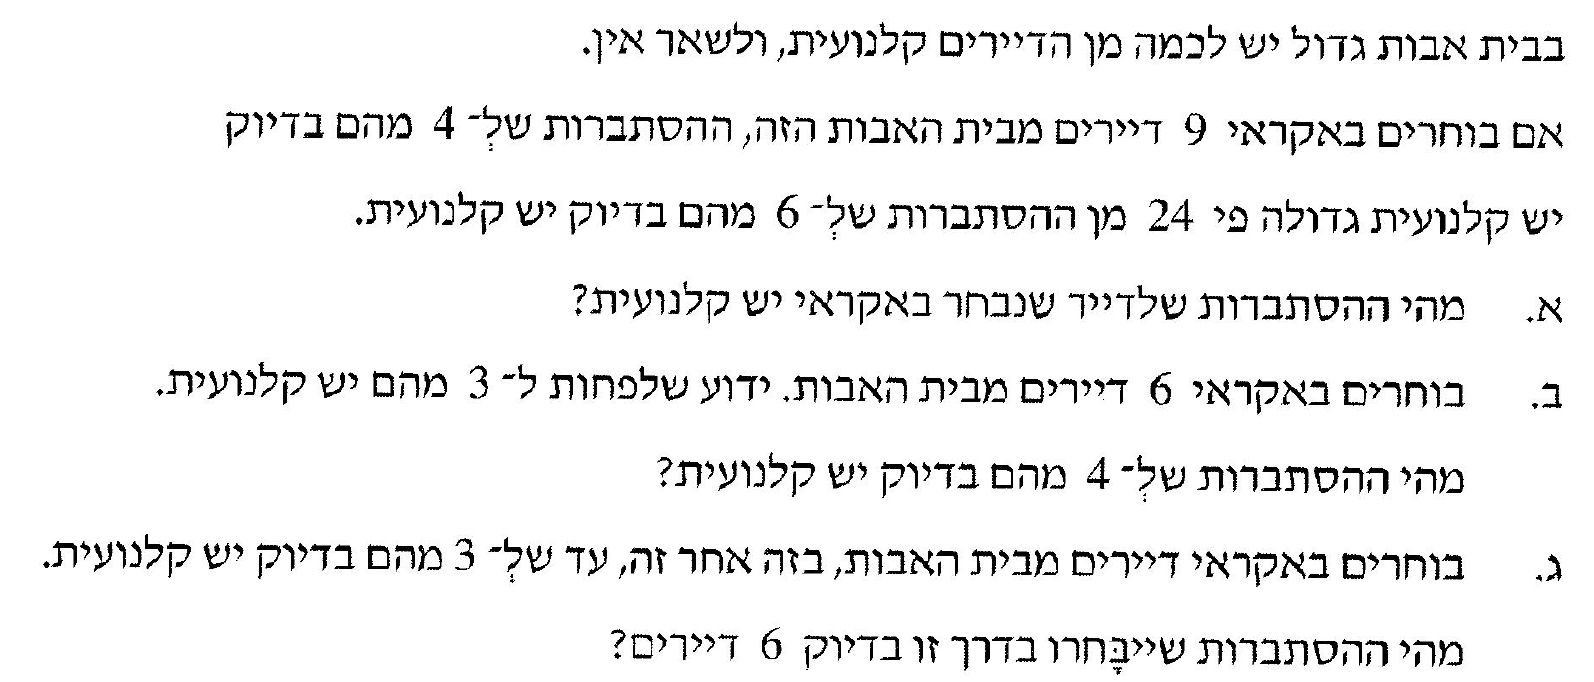
\includegraphics[width=.95\textwidth]{summer-2017a-3}
\end{center}

סעיף א. נסמן ב-%
$D$
את האירוע "לדייר יש קלנועית" ואת ההסתברות של האירוע ב-%
$p$.
נתון ש:
\[
{9\choose 4} p^4 (1-p)^5=24 {9\choose 6} p^6 (1-p)^3\,.
\]
נפשט ונקבל משוואה ריבועית:
\[
15p^2+2p-1=0\,,
\]
עם שני פתרונות
$p=\frac{1}{5},-\frac{1}{3}$.
הסתברות חייבת להיות לא-שלילית ולכן התשובה היא 
$p=\frac{1}{5}=0.2$.

סעיף ב. המילים
"\textbf{ידוע ש-}"
מכוונות להסתברות מותנית:
\[
P(D=4/D\ge3) = \frac{P(D=4\cap D\ge 3)}{P(D\ge 3)}\,.
\]
כאשר יש חפיפה בין שני ביטויים בחיתוך אפשר לפשט אותו. ברור שאם ערך גדול או שווה
$3$
\textbf{וגם}
שווה ל-%
$4$
אז הוא שווה ל-%
$4$:
\[
P(D=4/D\ge3) =\frac{P(D=4)}{P(D\ge 3)}\,.
\]
לפי נוסחת ברנולי:
\[
P(D=4)={6\choose 4} 0.2^4 (1-0.2)^2= 0.01536\,.
\]
את הערך של
$P(D\ge 3)$
אפשר לחשב בשתי דרכים, בצורה ישירה או כאחד פחות המשלים. נבחר את האפשרות השנייה כי יש פחות גורמים בביטוי:
\[
1-0.2^0(1-0.2)^6-{6\choose 1}0.2^1(1-0.2)^5 - {6 \choose 2} 0.2^2(1-0.2)^4=0.099\,,
\]
והתשובה היא
$\displaystyle\frac{0.01536}{0.099}=0.15534$.

סעיף ג. הבחירה 
\textbf{האחרונה} 
תהיה "הצלחה" ויהיו שתי "הצלחות" בחמשת הבחירות הקודמות:
\[
\overbrace{\pm\;\pm\;\pm\;\pm\;\pm}^{2/5}\quad\quad \overbrace{+}^{1/1}\,.
\]
התשובה מתקבלת מנוסחת ברנולי לבחירות הראשונות כפול ההסתברות
$p$
לבחירה האחרונה:
\[
\left[{5\choose 2}0.2^2 (1-.02)^3\right]\cdot 0.2=0.04096\,.
\]

%%%%%%%%%%%%%%%%%%%%%%%%%%%%%%%%%%%%%%%%%%%%%%%%%%%%%%%%%%%%%%%%%%%
\newpage

\textbf{\R{
קיץ תשע"ז, מועד ב
}}

\begin{center}
\selectlanguage{english}
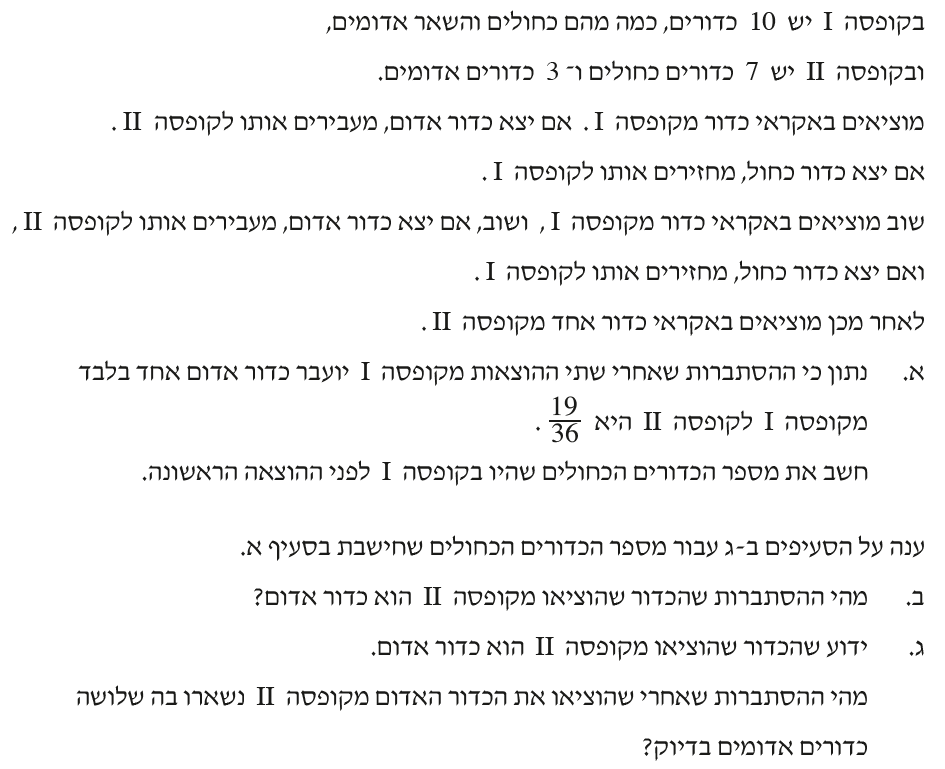
\includegraphics[width=.95\textwidth]{summer-2017b-3}
\end{center}

המילים "מוציאים באקראי
$\ldots$
\textbf{ולאחר מכן}
שוב מוציאים באקראי" מכוונות לשימוש בעץ. נסמן ב-%
\textsf{b}
את מספר הכדורים הכחולים בקופסה 
$I$.
באיור~%
\L{\ref{fig.summer-2017b.1}},
בכל צומת רשום שני זוגות של מספרים: מספר הכדורים האדומים ומספר הכדורים הכחולים בקופסה
$I$,
ומתחתיו מספר הכדורים האדומים ומספר הכדורים הכחולים בקופסה
$II$.

סעיף א. הכוכביות מסמנות את שתי האפשרויות בהן הוצאנו כדור אדום אחד בדיוק מקופסה
\textsf{I}.
\begin{figure}
\begin{center}
\selectlanguage{english}
\begin{tikzpicture}
[grow=right,
level 1/.append style={font=\sffamily,text width=2cm,level distance=5cm,sibling distance=10em},
level 2/.append style={font=\sffamily,text width=2cm,level distance=7cm,sibling distance=6em}]
\node[font=\sffamily,text width=2cm] {(10-b,b)\\(3,7)} % root
child {
  node {(10-b,b)\\(3,7)}
    child {
      node {(10-b,b)\\(3,7)}
      edge from parent node[below] {\R{כחול}}
        node[above,xshift=16mm,yshift=-2mm] {$\frac{b}{10}$}
    }
    child {
      node {(9-b,b)\ *\\(4,7)}
      edge from parent node[above] {\R{אדום}}
        node[below,xshift=16mm,yshift=2mm] {$\frac{10-b}{10}$}
    }
    edge from parent node[below] {\R{כחול}} node[above,xshift=8mm,yshift=0mm] {$\frac{b}{10}$}
}
child { 
  node {(9-b,b)\\(4,7)}
    child {
      node {(9-b,b)\ *\\(4,7)}
      edge from parent node[below] {\R{כחול}}
        node[above,xshift=16mm,yshift=-2mm] {$\frac{b}{9}$}
    }
    child {
      node {(8-b,b)\\(5,7)}
      edge from parent node[above] {\R{אדום}}
        node[below,xshift=16mm,yshift=2mm] {$\frac{9-b}{9}$}
    }
    edge from parent node[above] {\R{אדום}} 
      node[below,xshift=8mm,yshift=0mm] {$\frac{10-b}{10}$}
};
\end{tikzpicture}
\selectlanguage{hebrew}
\setlength{\belowcaptionskip}{-4ex}
\caption{עץ ההסתברויות של הוצאת הכדורים מקופסה $I$}\label{fig.summer-2017b.1}
\end{center}
\end{figure}
נשווה את הסתברות הנתונה לסכום ההסתברויות של שני המסלולים:
\[
\frac{10-b}{10}\cdot\frac{b}{9} + \frac{b}{10}\cdot\frac{10-b}{10} = \frac{19}{36}\,.
\]
נפשט ונקבל משוואה ריבועית 
$b^2-10b+25=0$
שיש לה פתרון אחד
$b=5$.

סעיף ב. לאחר הצבת 
$b=5$,
נקבל עבור כל מצב את מספר הכדורים האדומים וכחולים בקופסה
$II$,
נוכל לחשב את ההסתברויות להוצאת כדור אדום מקופסה
$II$,
ונסכם את ההסתברויות לאחר הכפלתן בהסתברות להגיע לכל אחד מהמצבים:
\[
\renewcommand{\arraystretch}{2}
\begin{array}{l}
\displaystyle\left(\frac{5}{10}\cdot\frac{4}{9}\right)\left(\frac{5}{5+7}\right)+
\left(\frac{5}{10}\cdot\frac{5}{9}\right)\left(\frac{4}{4+7}\right)+\\
\displaystyle\left(\frac{5}{10}\cdot\frac{5}{10}\right)\left(\frac{4}{4+7}\right)+
\left(\frac{5}{10}\cdot\frac{5}{10}\right)\left(\frac{3}{3+7}\right)
=0.3595\,.
\end{array}
\]

סעיף ג. המילים 
"\textbf{ידוע ש-}"
מכוונת להסתברות מותנית:
\vspace{-4ex}
\[
\renewcommand{\arraystretch}{2}
\begin{array}{c}
P(II\ \textrm{\R{נשארו שלושה אדומים בקופסה}}/II\ \textrm{\R{הוציאו כדור אדום מקופסה}}) =\\
\displaystyle\frac{P(II\ \textrm{\R{נשארו שלושה אדומים בקופסה}} \cap II\ \textrm{\R{הוציאו כדור אדום מקופסה}})}{P(II\ \textrm{\R{הוציאו כדור אדום מקופסה}})}
\end{array}
\]
ישארו שלושה כדורים אדומים רק אם היו אברעה כדורים אדומים לפני הבחירה. ההסתברות במנה היא ההסתברות )הנתונה!( שנגיע לאחד המצבים המסומנים בכוכבית כפול ההסתברות לבחור אדום מקופסה 
$II$,
וחישבנו את ההסתברות במכנה בסעיף ב. התשובה היא:
\[
\frac{\displaystyle\frac{19}{36}\cdot\frac{4}{11}}{0.3595}=0.53385\,.
\]

%%%%%%%%%%%%%%%%%%%%%%%%%%%%%%%%%%%%%%%%%%%%%%%%%%%%%%%%%%%%%%%%%%%
\newpage

\textbf{\R{
חורף תשע"ו
}}

\begin{center}
\selectlanguage{english}
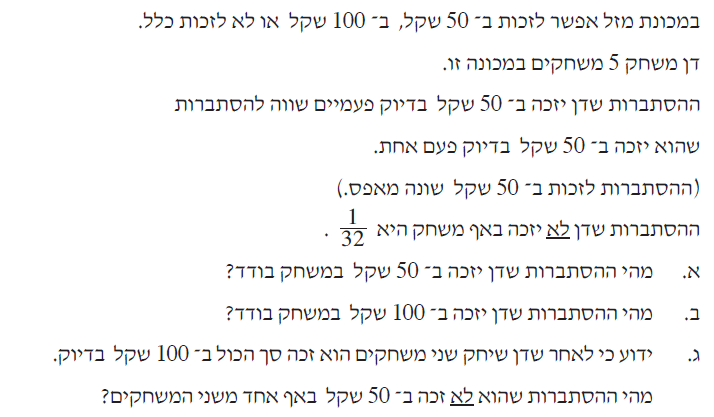
\includegraphics[width=.85\textwidth]{winter-2016-3}
\end{center}
סעיף א. ההסתברות שדן לא יזכה באף אחד מחמישת המשחקים היא 
$P(0)^5$.
נתון שערך זה הוא 
$\frac{1}{32}$,
ולכן 
$P(0)=\frac{1}{2}$.
לפי המידע הנתון:
\begin{eqnarray*}
{5\choose 2} P(50)^2 (1-P(50))^3 &=& {5\choose 1} P(50) (1-P(50))^4\\
P(50)&=&\frac{1}{3}\,.
\end{eqnarray*}
סעיף ב. לפי ההסתברות המשלימה:
$\displaystyle P(100) = 1 - P(0) - P(50) = 1-\frac{1}{2}-\frac{1}{3}=\frac{1}{6}$.

סעיף ג. המילים
"\textbf{ידוע כי}"
מכוונות להסתברות מותנית:
\vspace{-4ex}
\[
\renewcommand{\arraystretch}{2}
\begin{array}{c}
P(\textrm{\R{ באף משחק}}50\textrm{\R{לא זכה ב-}}
/
\textrm{\R{ בשני משחקים}}
100\textrm{\R{זכה ב-}}) =\\
\displaystyle\frac{
P(\textrm{\R{ באף משחק}}50\textrm{\R{לא זכה ב-}}
\cap
\textrm{\R{ בשני משחקים}}
100\textrm{\R{זכה ב-}})
}
{P(
\textrm{\R{ בשני משחקים}}
100\textrm{\R{זכה ב-}})}\,.
\end{array}
\]
נתבונן בעץ המציג את תוצאות שני המשחקים )איור~%
\L{\ref{fig.winter-2017.1}}(.
סימנו את המסלולים שבהם דן זכה ב-%
$100$
והמסלולים בהם דן לא זכה ב-%
$50$
באף אחד משני המשחקים.
\begin{figure}
\begin{center}
\selectlanguage{english}
\begin{tikzpicture}
[grow=right,
level 1/.append style={font=\sffamily,level distance=4cm,sibling distance=6em},
level 2/.append style={font=\sffamily,level distance=5cm,sibling distance=2em}]
\node[left] {$0$} % root
child {
  node[right] {$100$}
    child {
      node[right] {$200\quad \neq 50$}
      edge from parent node[below] {$1/6$}
    }
    child {
      node[right] {$150$}
      edge from parent node[below,xshift=4em] {$1/3$}
    }
    child {
      node[right] {$100\quad =100,\quad \neq 50$}
      edge from parent node[above] {$1/2$}
    }
    edge from parent node[below,yshift=-2mm] {$1/6$}
}
child {
  node[right] {$50$}
    child {
      node[right] {$150$}
      edge from parent node[below] {$1/6$}
    }
    child {
      node[right] {$100\quad =100$}
      edge from parent node[below,xshift=4em] {$1/3$}
    }
    child {
      node[right] {$50$}
      edge from parent node[above] {$1/2$}
    }
    edge from parent node[below] {$1/3$}
}
child {
  node[right] {$0$}
    child {
      node[right] {$100\quad =100,\quad \neq 50$}
      edge from parent node[below] {$1/6$}
    }
    child {
      node[right] {$50$}
      edge from parent node[below,xshift=4em] {$1/3$}
    }
    child {
      node[right] {$0\quad \neq 50$}
      edge from parent node[above] {$1/2$}
    }
    edge from parent node[above,yshift=2mm] {$1/2$}
}
;
\end{tikzpicture}
\selectlanguage{hebrew}
\setlength{\belowcaptionskip}{-6ex}
\caption{עץ ההסתברויות של המשחקים}\label{fig.winter-2017.1}
\end{center}
\end{figure}
חישוב ההסתברות המותנית:
\[
\frac{\displaystyle\frac{1}{2}\cdot\frac{1}{6} + \frac{1}{6}\cdot \frac{1}{2}}{\displaystyle\frac{1}{2}\cdot\frac{1}{6} + \frac{1}{3}\cdot \frac{1}{3}+ \frac{1}{6}\cdot \frac{1}{2}}  =  \frac{\displaystyle\frac{1}{6}}{\displaystyle\frac{5}{18}}=\frac{3}{5}\,.
\]

%%%%%%%%%%%%%%%%%%%%%%%%%%%%%%%%%%%%%%%%%%%%%%%%%%%%%%%%%%%%%%%%%%%
\newpage

\textbf{\R{
קיץ תשע"ו, מועד א
}}

\begin{center}
\selectlanguage{english}
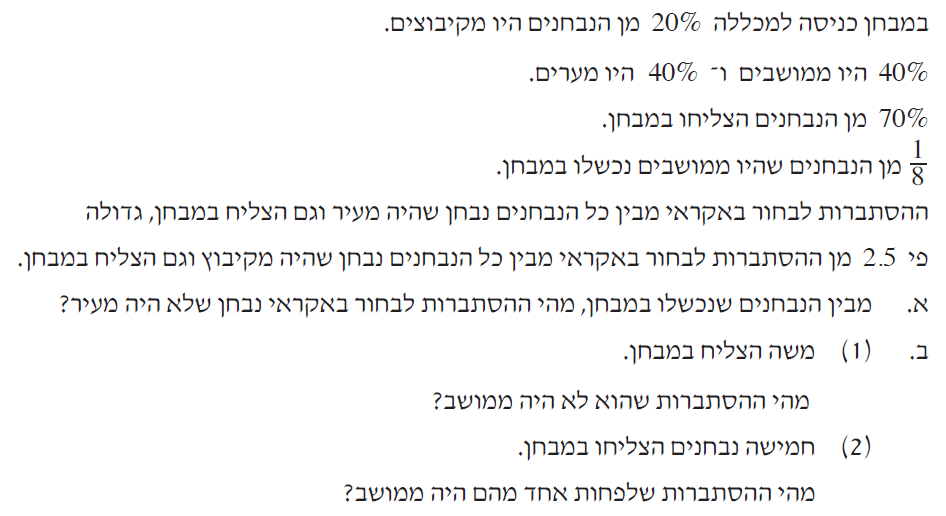
\includegraphics[width=.95\textwidth]{summer-2016a-3}
\end{center}

נסמן 
$=S$
נבחנים שהצליחו,
$=K$
נבחנים מקיבוצים,
$=M$
נבחנים ממושבים,
$=E$
נבחנים מערים. ההסתברויות הנתונות הן:
\[
P(K)=0.20,\;P(M)=0.40,\;P(E)=0.40,\;P(S)=0.70\,.
\]
נחשב את שאר ההסתברויות. לפי הסתברות משלימה
$P(\overline{S})=1-P(S)=0.30$.
נתון:
\[
P(\overline{S}/M)=P(\overline{S}\cap M) / P(M)=\frac{1}{8}\,,
\]
ולכן:
\[
P(\overline{S}\cap M)=\frac{1}{8}P(M)=0.05\,.
\]
לפי ההגדרה:
\[
P(S)=P(K\cap S) + P(M\cap S) + P(E\cap S)\,.
\]
נסמן
$P(K\cap S)=p$,
ההסתברות שנבחנים מקיבוצים הצליחו. נתון:
\[
P(E\cap S)=2.5P(K\cap S)=2.5p\,,
\]
ולכן:
\[
0.70=p+(0.40-0.05)+2.5p\,,
\]
ו-%
$p=0.1$.

שימו לב שהמילים 
"$\frac{1}{8}$
\textbf{מן}
הנבחנים שהיו ממושבים נכשלו" מכוונות להסתברות מותנית, לעומת המילים "ההסתברות לבחור באקראי
\textbf{מבין כל}
הנבחנים נבחן שהיה מהעיר
\textbf{וגם}
הצליח במבחן" מכוונות לחיתוך הסתברויות. המילה "מבין" בדרך כלל מכוונת להסתברות מותנית, אבל כאשר "מבין" מתייחס ל-%
"\textbf{כל}
הנבחנים" אין הסתברות מותנית. לחילופין, ההסתברות לבחור אחד "מכל הנבחנים" היא 
$1$,
ולכן:
\[
P(E\cap S/\textrm{\R{כל הנבחנים}})=
\frac{(P(E\cap S)\cap \textrm{\R{כל הנבחנים}})}
{P(\textrm{\R{כל הנבחנים}})} = 
\frac{P(E\cap S)}{1}=P(E\cap S)\,.
\]
נסכם את המידע בטבלה:
\begin{center}
\selectlanguage{english}
\begin{tikzpicture}[scale=1.25]
\draw (0,0) grid (4,3);
\node at (3.5,3.3) {$\bm{K}$};
\node at (2.5,3.3) {$\bm{M}$};
\node at (1.5,3.3) {$\bm{E}$};
\node at (4.3,2.5) {$\bm{S}$};
\node at (4.3,1.5) {$\bover{S}$};

\node at (0.5,2.5) {$0.70$};
\node at (0.5,1.5) {$0.30$};
\node at (0.5,0.5) {$1.0$};

\node at (1.5,2.5) {$0.25$};
\node at (1.5,1.5) {$0.15$};
\node at (1.5,0.5) {$0.40$};

\node at (2.5,2.5) {$0.35$};
\node at (2.5,1.5) {$0.05$};
\node at (2.5,0.5) {$0.40$};

\node at (3.5,2.5) {$0.10$};
\node at (3.5,1.5) {$0.10$};
\node at (3.5,0.5) {$0.20$};
\end{tikzpicture}
\end{center}
סעיף א. לפי הנוסחה להסתברות מותנית:
\[
P(\overline{E}/\overline{S})=P((K\cup M)/\overline{S}) = \frac{P(K\cap \overline{S})+P(M\cap \overline{S})}{P(\overline{S})}=\frac{0.10+0.05}{0.30}=\frac{1}{2}\,.
\]
סעיף ב
$(1)$.
לפי הנוסחה להסתברות מותנית:
\[
P(\overline{M}/S)=P((K\cup E)/S) = \frac{P(K\cap S)+P(E\cap S)}{P(S)}=\frac{0.10+0.25}{0.70}=\frac{1}{2}\,.
\]
סעיף ב
$(2)$.
%את ההסתברות שנבחן שהצליח המושב ניתן לחשב בדיוק כמו בסעיף ב
%$(1)$,
%אבל ההסתברות זו היא המשלים של ההסתברות שחושב שם
%$P(M/S)=1-P(\overline{M}/S)=1-\frac{1}{2}=\frac{1}{2}$.
"לפחות אחד ממושב" הוא המשלים ל-"כולם לא מהמושב":
\[
1-P(\overline{M}/S)^5=1-\left(\frac{1}{2}\right)^2=\frac{31}{32}\,.
\]
%%%%%%%%%%%%%%%%%%%%%%%%%%%%%%%%%%%%%%%%%%%%%%%%%%%%%%%%%%%%%%%%%%%
\newpage

\textbf{\R{
קיץ תשע"ו, מועד ב
}}

\begin{center}
\selectlanguage{english}
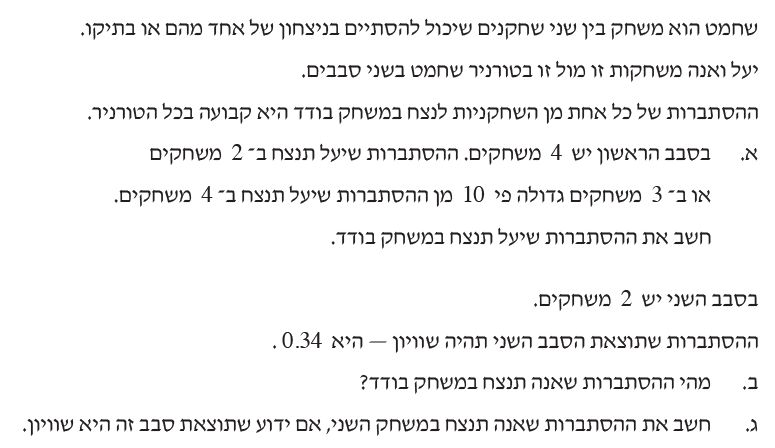
\includegraphics[width=.86\textwidth]{summer-2016b-3}
\end{center}
נסמן:
$=y$
ההסתברות שיעל תנצח במשחק בודד, 
$=a$
ההסתברות שאנה תנצח במשחק בודד.

סעיף א. לפי המידע הנתון:
\[
{4 \choose 2}y^2(1-y)^2 + {4\choose 3}y^3(1-y) = 10\cdot {4\choose 4}y^4(1-y)^0\,.
\]
נפשט ונקבל משוואה ריבועית
$4y^2+4y-3=0$
שהשורש החיובי היחיד שלה היא
$y=\frac{1}{2}$.

סעיף ב. כדאי לצייר עץ של האירועים, אבל אוותר עליו בשאלה זו כי המצב פשוט. האפשרויות לקבל שוויון הן: )א( ניצחון אחד לאנה וליעל, או )ב( תיקן בשני המשחקים. ההסתברות לתיקו היא המשלים לסכום ההסתברויות שאחת מהן תנצח:
\[
{2 \choose 1}ya + (1-(y+a))^2 = 0.34\,.
\]
נציב 
$y=\frac{1}{2}$
ונקבל
$a=0.3$.

סעיף ג. המילים
"\textbf{אם ידוע ש-}"
מכוונות להסתברות מותנית:
\vspace{-2ex}
\[
\renewcommand{\arraystretch}{2}
\begin{array}{c}
P(\textrm{\R{אנה תנצח במשחק השני}} / \textrm{\R{תוצאת הסבב השני היא שוויון}})=\\
\displaystyle\frac{
P(\textrm{\R{אנה תנצח במשחק השני}} \cap \textrm{\R{תוצאת הסבב השני היא שוויון}})
}
{P(\textrm{\R{תוצאת הסבב השני היא שוויון}})}\,.
\end{array}
\]
ההסתברות לשיוון בסבב השני נתונה. אם אנה תנצח במשחק השני, יהיה שוויון רק אם גם יעל תנצח במשחק הראשון:
\vspace{-1ex}
\[
\frac{ya}{.34}=\frac{\displaystyle\frac{1}{2}\cdot 0.3}{.34}=0.4412\,.
\]
שימו לב שלא צריכים
$2 \choose 1$
כי האירוע הוא שאנה תנצח במשחק 
\textbf{השני}
ויעל תנצח במשחק
\textbf{הראשון}.
%%%%%%%%%%%%%%%%%%%%%%%%%%%%%%%%%%%%%%%%%%%%%%%%%%%%%%%%%%%%%%%%%%%
\newpage

\textbf{\R{
חורף תשע"ה
}}

\begin{center}
\selectlanguage{english}
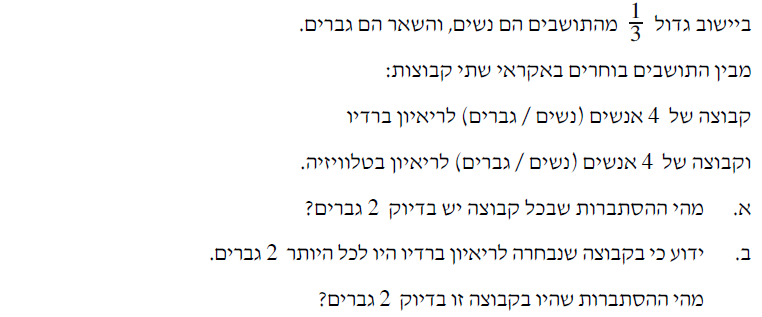
\includegraphics[width=.85\textwidth]{winter-2015-3}
\end{center}

"יישוב גדול" אומר לי שניתן לבחור מספר רב של תושבים, לפחות שמונה תושבים כפי שנדרש.

סעיף א. כל קבוצה היא בחירה בלתי תלוייה:
\[
{4 \choose 2}\left(\frac{2}{3}\right)^2\left(1-\frac{2}{3}\right)^2=\frac{8}{27}\,,
\]
וכדי לקבל את ההסתברות שלשתי הקבוצות יהיו בדיוק שני גברים, נעלה ערך זה בריבוע:
\[
\left(\frac{8}{27}\right)^2=\frac{64}{729}\,.
\]
סעיף ב. המילים
"\textbf{ידוע כי}"
מכוונות להסתברות מותנית:
\vspace{-4ex}
\[
\renewcommand{\arraystretch}{2}
\begin{array}{c}
P(\textrm{\R{בדיוק שני גברים}} / \textrm{\R{לכל היותר שני גברים}})=\\
\displaystyle\frac{
P(\textrm{\R{בדיוק שני גברים}} \cap \textrm{\R{לכל היותר שני גברים}})
}
{P(\textrm{\R{לכל היותר שני גברים}})}\,.
\end{array}
\]
החיתוך במנה שקולה ל-"בדיוק שני גברים" )שחישבנו בסעיף א(, כי "לכל היותר שני גברים" היא 
$0,1,2$
גברים. "לכל היותר שני גברים" הוא הסכום של שלוש נוסחאות ברנולי:
\[
\left(\frac{2}{3}\right)^0\left(\frac{1}{3}\right)^4 + {4\choose 1}\left(\frac{2}{3}\right)^1\left(\frac{1}{3}\right)^3 + {4\choose 2}\left(\frac{2}{3}\right)^2\left(\frac{1}{3}\right)^2=\frac{11}{27}\,
\]
והתשובה לשאלה היא:
\[
\frac{8/27}{11/27}=\frac{8}{11}\,.
\]

%%%%%%%%%%%%%%%%%%%%%%%%%%%%%%%%%%%%%%%%%%%%%%%%%%%%%%%%%%%%%%%%%%%
\newpage

\textbf{\R{
קיץ תשע"ה, מועד א
}}

\begin{center}
\selectlanguage{english}
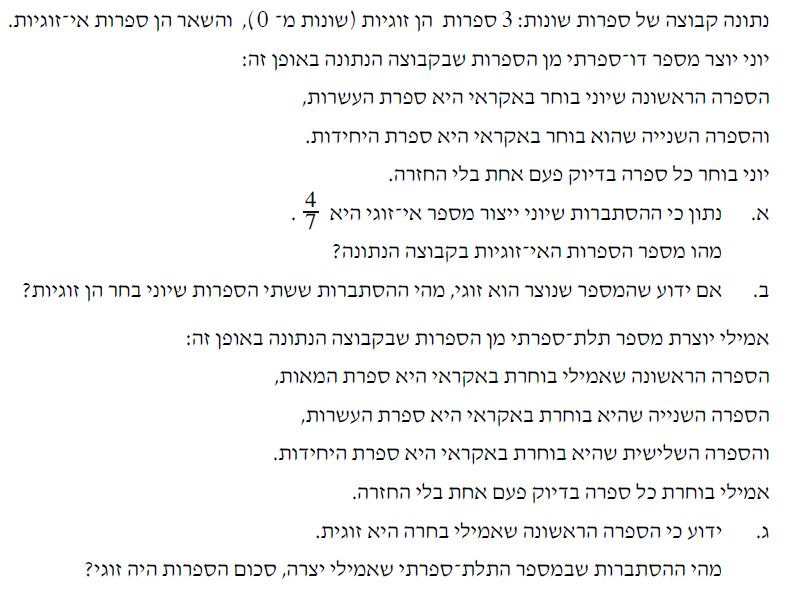
\includegraphics[width=.85\textwidth]{summer-2015a-3}
\end{center}

נסמן 
$=n$
מספר הספרות בקבוצה. מספר הזוגיים 
$3=$,
ומספר האי-זוגיים
$n-3=$.
השאלה מתארת בחירה של "הספרה הראשונה" ואחר כך "הספרה הראשונה", תיאור המכוון לעץ הסתברויות )איור~%
\L{\ref{fig.summer-2015a.1}}(.
כדי לפשט את האיור רשמתי בכל צומת את ההסתברויות ולא את מספר הספרות.

\begin{figure}[H]
\begin{center}
\selectlanguage{english}
\begin{tikzpicture}
[grow=right,
level 1/.append style={text width=2cm,level distance=3.5cm,sibling distance=8em},
level 2/.append style={text width=2.5cm,level distance=4.5cm,sibling distance=4em}]
\node[text width=2cm] {$\left(\frac{3}{n},\frac{n-3}{n}\right)$} % root
child {
  node {$\left(\frac{3}{n-1},\frac{n-4}{n-1}\right)$}
    child {
      node {$\left(\frac{3}{n-2},\frac{n-5}{n-2}\right)\quad *$}
      edge from parent node[below,xshift=5mm,yshift=-1mm] {\R{אי-זוגי}}
    }
    child {
      node {$\left(\frac{2}{n-2},\frac{n-4}{n-2}\right)$}
      edge from parent node[above,xshift=5mm,yshift=1mm] {\R{זוגי}}
    }
    edge from parent node[below,yshift=-1mm] {\R{אי-זוגי}}
}
child { 
  node {$\left(\frac{2}{n-1},\frac{n-3}{n-1}\right)$}
    child {
      node {$\left(\frac{2}{n-2},\frac{n-4}{n-2}\right)\quad *$}
      edge from parent node[below,xshift=5mm,yshift=-1mm] {\R{אי-זוגי}}
    }
    child {
      node {$\left(\frac{1}{n-2},\frac{n-3}{n-2}\right)$}
      edge from parent node[above,xshift=5mm,yshift=1mm] {\R{זוגי}}
    }
    edge from parent node[above] {\R{זוגי}}
};
\end{tikzpicture}
\selectlanguage{hebrew}
\setlength{\belowcaptionskip}{-8ex}
\caption{עץ ההסתברויות של בחירת הספרות}\label{fig.summer-2015a.1}
\end{center}
\end{figure}

סעיף א. המספר יהיה אי-זוגי אם 
\textbf{הבחירה השנייה}
היא של ספרה אי-זוגית. המסלולים האלה מסומנים בכוכביות באיור. נשווה את סכום ההסתברויות של המסלולים לערך הנתון:
\[
\frac{3}{n}\cdot\frac{n-3}{n-1} \;+\; \frac{n-3}{n}\cdot\frac{n-4}{n-1} = \frac{4}{7}\,.
\]
נפשט ונקבל משוואה ריבועית
$n^2-8n+7=0$
שיש לה שני פתרונות לא-שליליים
$n=1,n=7$.
נתון שיש לפחות שלוש ספרות, לכן מספר הספרות הוא
$7$.
שימו לב שהשאלה מבקשת את מספר הספרות 
\textbf{האי-זוגיות}
ולכן התשובה היא
$7-3=4$.

סעיף ב. המילים 
"\textbf{אם ידוע ש-}"
מכוונות להסתברות מותנית. במספר זוגי הספרה האחרונה זוגית:
\vspace{-3ex}
\[
\renewcommand{\arraystretch}{2}
\begin{array}{c}
P(\textrm{\R{שתי ספרות זוגיות}} / \textrm{\R{ספרה אחרונה זוגית}})=\\
\displaystyle\frac{
P(\textrm{\R{שתי ספרות זוגיות}} \cap \textrm{\R{ספרה אחרונה זוגית}})
}
{P(\textrm{\R{ספרה אחרונה זוגית}})}=\\
\displaystyle\frac{
P(\textrm{\R{שתי ספרות זוגיות}})
}
{P(\textrm{\R{ספרה אחרונה זוגית}})}\,.
\end{array}
\]
את החיתוך אפשר לפשט כי אם שתי הספרות זוגיות, הספרה האחרונה חייבת להיות זוגית.

ניתן לחשב את ההסתברות "ספרה אחרונה זוגית" במכנה לפי המידע בעץ ההסתברויות או פשוט לשים לב שהיא המשלימה לערך הנתון בסעיף א של "הספרה האחרונה אי-זוגית". נחשב את ההסתברות במנה לפי המסלול הבודד בעץ ההסתברויות )איור~
\L{\ref{fig.summer-2015a.2}}(
של בחירה של שתי ספרות זוגיות:
\[
\frac{\displaystyle\frac{3}{7}\cdot\frac{2}{6}}{1-\displaystyle\frac{4}{7}}=\frac{1}{3}\,.
\]
סעיף ג. הסכום יהיה זוגי רק אם שתי הספרות האחרונת הן זוגיות או אי-זוגיות:
\begin{eqnarray*}
2k_1+2k_2+2k_3&=&2(k_1+k_2+k_3)\\
2k_1+2(k_2+1)+2(k_3+1)&=&2(k_1+k_2+k_3+1)\,.
\end{eqnarray*}
שני האירועים )בחירת הספרות( בלתי תלויים, ולכן אפשר לבטא את החיתוך כמכפלה:
\vspace{-3ex}
\[
\renewcommand{\arraystretch}{2}
\begin{array}{c}
P(\textrm{\R{סכום זוגי}} / \textrm{\R{ספרה ראשונה זוגית}})=\\
\displaystyle\frac{
P(\textrm{\R{סכום זוגי}} \cap \textrm{\R{ספרה ראשונה זוגית}})
}
{P(\textrm{\R{ספרה ראשונה זוגית}})}=\\
\displaystyle\frac{
P(\textrm{\R{סכום זוגי}}) \cdot P(\textrm{\R{ספרה ראשונה זוגית}})
}
{P(\textrm{\R{ספרה ראשונה זוגית}})}=\\
P(\textrm{\R{סכום זוגי}})\,.
\end{array}
\]
שימו לב שלאחר הבחירה הראשונה של אמילי מספר הספרות הוא שש. לפי עץ ההסתברויות החדש )איור~
\L{\ref{fig.summer-2015a.3}}(
 ההסתברות היא:
\[
\frac{2}{6}\cdot\frac{1}{5}+\frac{4}{6}\cdot\frac{3}{5}=\frac{7}{15}\,.
\]

\begin{figure}[H]
\begin{center}
\selectlanguage{english}
\begin{tikzpicture}
[grow=right,
level 1/.append style={level distance=3cm,sibling distance=8em},
level 2/.append style={level distance=4cm,sibling distance=4em}]
\node {$\left(\frac{3}{7},\frac{4}{7}\right)$} % root
child {
  node {$\left(\frac{3}{6},\frac{3}{6}\right)$}
    child {
      node {$\left(\frac{3}{5},\frac{2}{5}\right)$}
      edge from parent node[below,xshift=5mm,yshift=-3mm] {\R{אי-זוגי}}
    }
    child {
      node {$\left(\frac{2}{5},\frac{3}{5}\right)$}
      edge from parent node[above,xshift=5mm,yshift=1mm] {\R{זוגי}}
    }
    edge from parent node[below,yshift=-3mm] {\R{אי-זוגי}}
}
child { 
  node {$\left(\frac{2}{6},\frac{4}{6}\right)$}
    child {
      node {$\left(\frac{2}{5},\frac{3}{5}\right)$}
      edge from parent node[below,xshift=5mm,yshift=-3mm] {\R{אי-זוגי}}
    }
    child {
      node {$\left(\frac{1}{5},\frac{4}{5}\right)\quad$ *}
      edge from parent node[above,xshift=5mm,yshift=1mm] {\R{זוגי} }
    }
    edge from parent node[above,yshift=2mm] {\R{זוגי}}
};
\end{tikzpicture}
\selectlanguage{hebrew}
\caption{עץ ההסתברויות של בחירת הספרות}\label{fig.summer-2015a.2}
\end{center}
\end{figure}
\begin{figure}[H]
\begin{center}
\selectlanguage{english}
\begin{tikzpicture}
[grow=right,
level 1/.append style={level distance=3cm,sibling distance=8em},
level 2/.append style={level distance=4cm,sibling distance=4em}]
\node {$\left(\frac{2}{6},\frac{4}{6}\right)$} % root
child {
  node {$\left(\frac{2}{5},\frac{3}{5}\right)$}
    child {
      node {$\left(\frac{2}{4},\frac{2}{4}\right)$}
      edge from parent node[below,xshift=5mm,yshift=-2mm] {\R{אי-זוגי}}
    }
    child {
      node {$\left(\frac{1}{4},\frac{3}{4}\right)$}
      edge from parent node[above,xshift=5mm,yshift=2mm] {\R{זוגי}}
    }
    edge from parent node[below,yshift=-3mm] {\R{אי-זוגי}}
}
child { 
  node {$\left(\frac{1}{5},\frac{4}{5}\right)$}
    child {
      node {$\left(\frac{1}{4},\frac{3}{4}\right)$}
      edge from parent node[below,xshift=5mm,yshift=-2mm] {\R{אי-זוגי}}
    }
    child {
      node {$\left(\frac{0}{4},\frac{4}{4}\right)\quad$ *}
      edge from parent node[above,xshift=5mm,yshift=2mm] {\R{זוגי}}
    }
    edge from parent node[above,yshift=2mm] {\R{זוגי}}
};
\end{tikzpicture}
\selectlanguage{hebrew}
\caption{עצי ההסתברויות של בחירת הספרות}\label{fig.summer-2015a.3}
\end{center}
\end{figure}
\clearpage

%%%%%%%%%%%%%%%%%%%%%%%%%%%%%%%%%%%%%%%%%%%%%%%%%%%%%%%%%%%%%%%%%%%
\newpage

\textbf{\R{
קיץ תשע"ה, מועד ב
}}

\begin{center}
\selectlanguage{english}
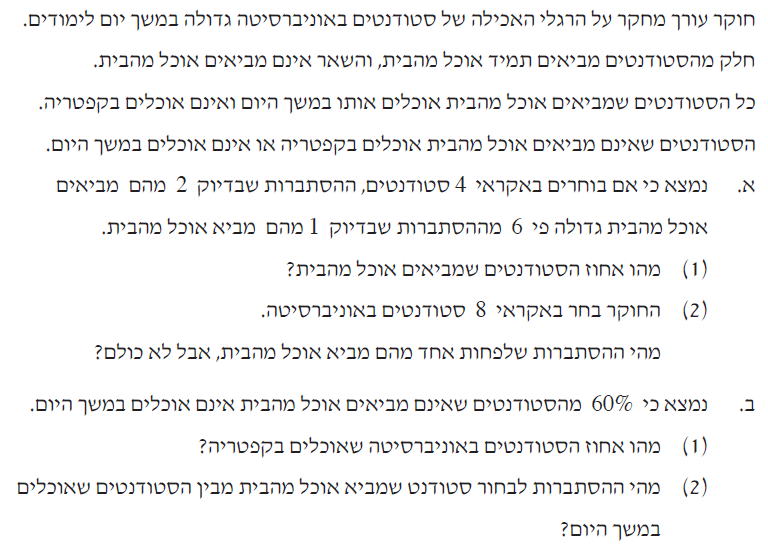
\includegraphics[width=.85\textwidth]{summer-2015b-3}
\end{center}

סעיף א
$(1)$.
נסמן
$=b$
ההסתברות להביא אוכל מהבית. לפי המידע הנתון:
\[
{4 \choose 2} b^2(1-b)^2 = 6\cdot {4 \choose 1} b (1-b)^3\,.
\]
פתרון המשוואה הוא 
$b=\frac{4}{5}$.

סעיף א
$(2)$.
"לפחות אחד אבל לא כולם" היא המשלים ל-"לא אפס ולא כולם":
\[
1-\left(\frac{1}{5}\right)^8-\left(\frac{4}{5}\right)^8=0.8322\,.
\]
סעיף ב
$(1)$.
בעץ ההסתברויות באיור~
\L{\ref{fig.summer-2015b.1}}
הכוכבית מראה את מהמסלול עבור "אוכל בקפטריה":
\[
\frac{1}{5}\cdot \frac{4}{10} = \frac{2}{25}\,.
\]
סעיף ב
$(2)$.
המילה
"\textbf{מבין}"
מכוונת להסתברות מותנית, כאשר קבוצת "מביא אוכל" היא תת-קבוצה של "אוכלים" והחישוב מצטמטם:
\[
%\vspace{-1ex}
\renewcommand{\arraystretch}{2}
\begin{array}{c}
P(\textrm{\R{מביא אוכל}} / \textrm{\R{אוכלים}})=\\
\displaystyle\frac{
P(\textrm{\R{מביא אוכל}} \cap \textrm{\R{אוכלים}})
}
{P(\textrm{\R{אוכלים}})}=\\
\displaystyle\frac{
P(\textrm{\R{מביא אוכל}})
}
{P(\textrm{\R{אוכלים}})}\,.
\end{array}
\]
החישוב הוא:
\[
\frac{4/5}{\displaystyle\frac{4}{5}+\frac{2}{25}}=\frac{10}{11}\,.
\]

\begin{figure}[H]
\begin{center}
\selectlanguage{english}
\begin{tikzpicture}
[grow=right,
level 1/.append style={level distance=3cm,sibling distance=6em},
level 2/.append style={text width=1cm,level distance=4cm,sibling distance=6em}]
\node[text width=1cm] {} % root
child {
  node {}
    edge from parent node[below,xshift=-5mm,yshift=-2mm] {\R{מביא מהבית}}
      node[above] {$\frac{4}{5}$}
}
child { 
  node {}
    child {
      node {*}
      edge from parent node[below,xshift=5mm,yshift=-1mm] {\R{אוכל בקפטריה}}
        node[above,xshift=8mm,yshift=-2mm] {$\frac{4}{10}$}
    }
    child {
      node {}
      edge from parent node[above,xshift=5mm,yshift=1mm] {\R{לא אוכל}}
        node[below,xshift=8mm,yshift=2mm] {$\frac{6}{10}$}
    }
    edge from parent node[above,xshift=-4mm,yshift=3mm] {\R{לא מביא מהבית}}
      node[below,xshift=4mm,yshift=2mm] {$\frac{1}{5}$}
};
\end{tikzpicture}
\selectlanguage{hebrew}
\setlength{\belowcaptionskip}{-4ex}
\caption{עץ ההסתברויות של אפשרויות האכילה}\label{fig.summer-2015b.1}
\end{center}
\end{figure}
%%%%%%%%%%%%%%%%%%%%%%%%%%%%%%%%%%%%%%%%%%%%%%%%%%%%%%%%%%%%%%%%%%%
%\newpage

\textbf{\R{
חורף תשע"ד
}}
\begin{center}
\selectlanguage{english}
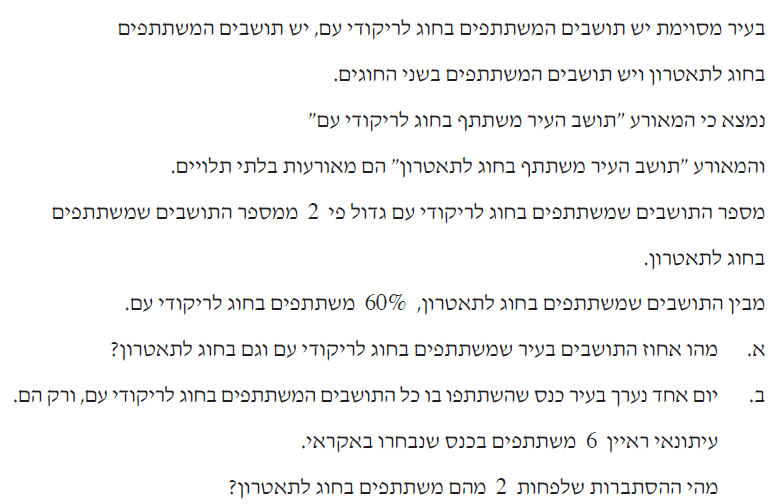
\includegraphics[width=.9\textwidth]{winter-2014-3}
\end{center}

נסמן
$=T$
מספר המשתתפים בתאטרון,
$=R$
מספר המשתתפים בריקודי עם. המילה 
"\textbf{מבין}"
מכוונת להתסברות מותנית. נתון
$P(R/T)=0.6$
וגם שהאירועים בלתי תלויים. נחשב:
\[
0.6=P(R/T)=\frac{P(R\cap T)}{P(T)}=\frac{P(R)\cdot P(T))}{P(T)}=P(R)\,.
\]
ביחד עם הנתון
$P(R)=2P(T)$
נתחיל למלא את הטבלה:
\begin{center}
\selectlanguage{english}
\begin{tikzpicture}[scale=1.25]
\draw (0,0) grid (3,3);
\node at (2.5,3.3) {$\bm{T}$};
\node at (1.5,3.3) {$\bover{T}$};
\node at (3.3,2.5) {$\bm{R}$};
\node at (3.3,1.5) {$\bover{R}$};
\node at (0.5,2.5) {$0.60$};
\node at (2.5,0.5) {$0.30$};
\node at (.5,.5) {$1.0$};
\node at (1.5,.5) {$0.70$};
\node at (.5,1.5) {$0.40$};
\end{tikzpicture}
\end{center}
שוב נסתמך על העובדה שהאירועים בלתי תלויים ונקבל:
\[
P(R\cap T)=P(R)\cdot P(T)=0.6\cdot 0.3=0.18\,,
\]
ואז יש לנו מספיק נתונים למלא את הטבלה:
\begin{center}
\selectlanguage{english}
\begin{tikzpicture}[scale=1.25]
\draw (0,0) grid (3,3);
\node at (2.5,3.3) {$\bm{T}$};
\node at (1.5,3.3) {$\bover{T}$};
\node at (3.3,2.5) {$\bm{R}$};
\node at (3.3,1.5) {$\bover{R}$};
\node at (2.5,2.5) {$0.18$};
\node at (0.5,2.5) {$0.60$};
\node at (1.5,2.5) {$0.42$};
\node at (0.5,1.5) {$0.40$};
\node at (0.5,0.5) {$1.0$};
\node at (1.5,0.5) {$0.70$};
\node at (2.5,0.5) {$0.30$};
\node at (1.5,1.5) {$0.28$};
\node at (2.5,1.5) {$0.12$};
\end{tikzpicture}
\end{center}
סעיף א. חישבנו ש-%
$P(R\cap T)=0.18$.

סעיף ב. המילים "כל התושבים המשתתפים בחוג לריקודי עם,
\textbf{ורק הם}"
מכוונות להסתברות מותנית. אם ידוע שתושב משתתף בריקודי עם, ההסתברות שהוא משתתף גם בתאטרון היא:
\[
P(T/R) = \frac{P(T\cap R)}{P(R)}= \frac{0.18}{.060} = 0.3\,.
\]
כדי לחשב "לפחות שניים" עדיף לחשב את המשלים ל-"אפס או אחד":
\[
1-{6\choose 0}(0.3)^0(0.7)^6 -{6\choose 1}(0.3)^1(0.7)^5=0.5798\,.
\]

%%%%%%%%%%%%%%%%%%%%%%%%%%%%%%%%%%%%%%%%%%%%%%%%%%%%%%%%%%%%%%%%%%%
\newpage

\textbf{\R{
קיץ תשע"ד, מועד א
}}

\begin{center}
\selectlanguage{english}
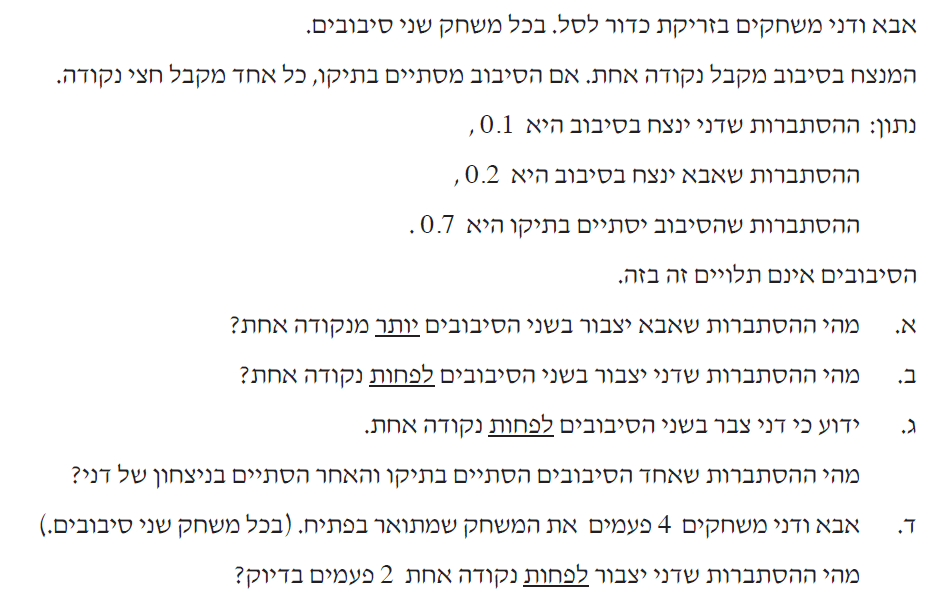
\includegraphics[width=.9\textwidth]{summer-2014a-3}
\end{center}
\vspace{-2ex}
סעיף א. איור~%
\L{\ref{fig.winter-2014.2}}
)למעלה( מראה את צבירת הנקודות של 
\textbf{אבא}
בשני הסיבובים. המצבים בהם אבא צובר
\textbf{יותר}
מנקודה אחת מסומנים בכוכבית. ההסתברות של האירוע היא:
\[
0.2\cdot 0.2 \,+\, 0.2\cdot 0.7 \,+\, 0.7\cdot 0.2 \,=\,0.32\,.
\]
סעיף ב. איור~%
\L{\ref{fig.winter-2014.2}}
)למטה( מראה את צבירת הנקודות של
\textbf{דני}
בשני הסיבובים. המצבים בהם דני צובר 
\textbf{לפחות}
נקודה אחת מסומנים בכוכבית. ההסתברות של האירוע היא:
\[
0.2\cdot 0.1 \,+\,0.1\cdot 0.2 \,+\, 0.1\cdot 0.1 \,+\,0.1\cdot 0.7 \,+\, 0.7\cdot 0.1\,+\,0.7\cdot 0.7\,=\,0.68\,.
\]
סעיף ג. המילים
"\textbf{ידוע כי}"
מכוונות להסתברות מותנית והחיתוך מצטמצם כי אם יש תיקו אחד וניצחון של דני אז דני צבר לפחות נקודה אחת:
\vspace{-2ex}
\[
\renewcommand{\arraystretch}{2}
\begin{array}{c}
P(\textrm{\R{תיקו אחד, ניצחון אחד לדני}} / \textrm{\R{דני צבר לפחות נקודה אחת}})=\\
\displaystyle\frac{
P(\textrm{\R{תיקו אחד, ניצחון אחד לדני}} \cap \textrm{\R{דני צבר לפחות נקודה אחת}})
}
{P(\textrm{\R{דני צבר לפחות נקודה אחת}})}=\\
\displaystyle\frac{
P(\textrm{\R{תיקו אחד, ניצחון אחד לדני}})
}
{P(\textrm{\R{דני צבר לפחות נקודה אחת}})}\,.
\end{array}
\]
נחשב את המנה על ידי חיבור ההסתברויות של שני מסלולים בעץ המסומנים ב-%
$\#$:
\[
\frac{0.1\cdot 0.7 \,+\, 0.7\cdot 0.1}{0.68} = .2059\,.
\]
סעיף ד. בסעיף ב חישבנו את ההסתברות של האירוע בכל סיבוב, ונשאר רק לחשב:
\vspace{-1ex}
\[
{4\choose 2}(0.68)^2 (0.32)^2= 0.2841\,.
\]
\vspace{-2ex}
\begin{figure}[H]
\begin{center}
\selectlanguage{english}
\begin{tikzpicture}
[align=left,grow=right,
level 1/.append style={font=\sffamily,level distance=3cm,sibling distance=8em},
level 2/.append style={font=\sffamily,level distance=4cm,sibling distance=3em}]
\node at (-1,3) {$0.2=$ \R{אבא}\\%
$0.1=$ \R{דני}\\%
$0.7=$ \R{תיקו}};
\node[left] {$0$} % root
child {
  node[right] {$\frac{1}{2}$}
    child {
      node[right] {$1$}
      edge from parent node[below,yshift=-1mm] {$0.7$}
    }
    child {
      node[right] {$\frac{1}{2}$}
      edge from parent node[below,xshift=4mm] {$0.1$}
    }
    child {
      node[right] {$1\frac{1}{2}\quad *$}
      edge from parent node[above,yshift=1mm] {$0.2$}
    }
    edge from parent node[below,yshift=-3mm] {$0.7$}
}
child {
  node[right] {$0$}
    child {
      node[right] {$\frac{1}{2}$}
      edge from parent node[below,yshift=-1mm] {$0.7$}
    }
    child {
      node[right] {$0$}
      edge from parent node[below,xshift=4mm] {$0.1$}
    }
    child {
      node[right] {$1$}
      edge from parent node[above,yshift=1mm] {$0.2$}
    }
    edge from parent node[below] {$0.1$}
}
child {
  node[right] {$1$}
    child {
      node[right] {$1\frac{1}{2}\quad *$}
      edge from parent node[below,yshift=-1mm] {$0.7$}
    }
    child {
      node[right] {$1$}
      edge from parent node[below,xshift=4mm] {$0.1$}
    }
    child {
      node[right] {$2\quad *$}
      edge from parent node[above,yshift=1mm] {$0.2$}
    }
    edge from parent node[above,yshift=3mm] {$0.2$}
};
\end{tikzpicture}
%\selectlanguage{hebrew}
%\caption{עץ ההסתברויות של המשחקים: צבירת נקודות של אבא}\label{fig.winter-2014.1}
%\end{center}
%\end{figure}
%
%
%\begin{figure}[H]
%\begin{center}
%\selectlanguage{english}
\bigskip

\begin{tikzpicture}
[grow=right,
level 1/.append style={font=\sffamily,level distance=3cm,sibling distance=8em},
level 2/.append style={font=\sffamily,level distance=4cm,sibling distance=3em}]
\node[left] {$0$} % root
child {
  node[right] {$\frac{1}{2}$}
    child {
      node[right] {$1\quad *$}
      edge from parent node[below,yshift=-1mm] {$0.7$}
    }
    child {
      node[right] {$1\frac{1}{2}\quad *\quad \#$}
      edge from parent node[below,xshift=4mm] {$0.1$}
    }
    child {
      node[right] {$\frac{1}{2}$}
      edge from parent node[above,yshift=1mm] {$0.2$}
    }
    edge from parent node[below,yshift=-3mm] {$0.7$}
}
child {
  node[right] {$1$}
    child {
      node[right] {$1\frac{1}{2}\quad *\quad \#$}
      edge from parent node[below,yshift=-1mm] {$0.7$}
    }
    child {
      node[right] {$2\quad *$}
      edge from parent node[below,xshift=4mm] {$0.1$}
    }
    child {
      node[right] {$1\quad *$}
      edge from parent node[above,yshift=1mm] {$0.2$}
    }
    edge from parent node[below] {$0.1$}
}
child {
  node[right] {$0$}
    child {
      node[right] {$\frac{1}{2}$}
      edge from parent node[below,yshift=-1mm] {$0.7$}
    }
    child {
      node[right] {$1\quad *$}
      edge from parent node[below,xshift=4mm] {$0.1$}
    }
    child {
      node[right] {$0$}
      edge from parent node[above,yshift=1mm] {$0.2$}
    }
    edge from parent node[above,yshift=3mm] {$0.2$}
};
\end{tikzpicture}
\selectlanguage{hebrew}
\setlength{\belowcaptionskip}{-4ex}
\caption{עץ ההסתברויות של צבירת נקודות של אבא )למעלה( ודני )למטה(}\label{fig.winter-2014.2}
\end{center}
\end{figure}


%%%%%%%%%%%%%%%%%%%%%%%%%%%%%%%%%%%%%%%%%%%%%%%%%%%%%%%%%%%%%%%%%%%

\textbf{\R{
קיץ תשע"ד, מועד ב
}}

\begin{center}
\selectlanguage{english}
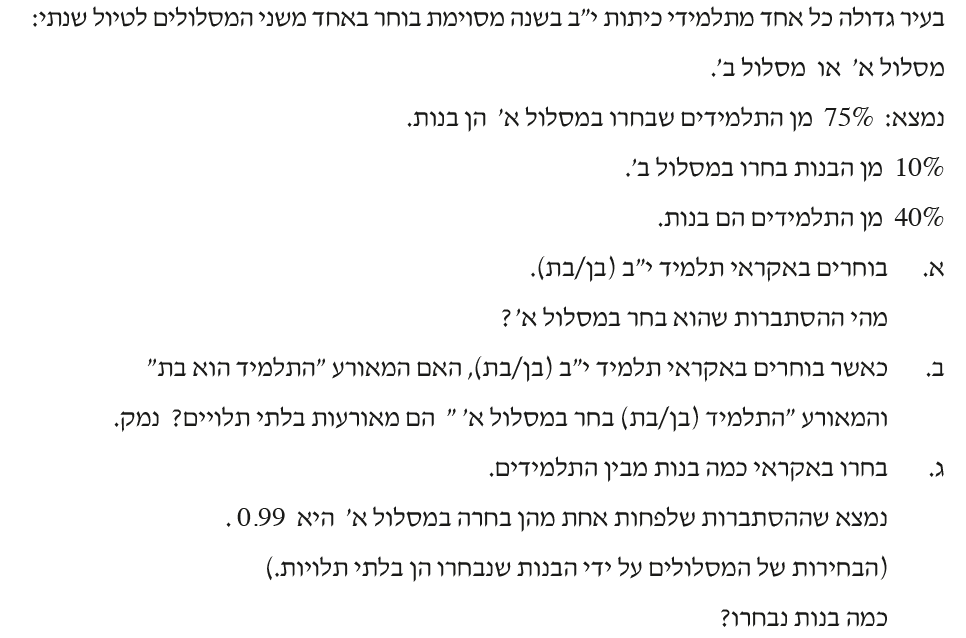
\includegraphics[width=.95\textwidth]{summer-2014b-3}
\end{center}

נמלא את הטבלה ממידע הנתון. נתון ש-% 
$0.4$
מהתלמידים הן בנות. 
$10\%$
מהם בחרו במסלול ב, ולכן נרשום
$0.1\times 0.4=.04$
מעל לתא עם הנתון הראשון. הסתברות המשלימה היא
$0.4-0.04=0.36$.
נתון ש-%
$75\%$
מהתלמידים שבחרו במסלול א הן בנות:
$0.75 \cdot \aleph = 0.36$,
ולכן 
$0.48$
מהתלמידים בחרו מסלול א. ניתן למלא את שאר התאים בטבלה לפי ההסתברויות המשלימות:
\begin{center}
\selectlanguage{english}
\begin{tikzpicture}[scale=2.2]
\draw (0,0) grid (3,3);
\node at (2.5,3.3) {\sffamily\bfseries \R{בנות}};
\node at (1.5,3.3) {\sffamily\bfseries \R{בנים}};
\node at (3.3,2.5) {\sffamily\bfseries \R{א}};
\node at (3.3,1.5) {\sffamily\bfseries \R{ב}};
\node at (2.5,2.7) {$.4-.04=$};
\node at (2.5,2.3) {$.36$};
\node at (0.5,2.7) {$.36/.75=$};
\node at (0.5,2.3) {$.48$};
\node at (1.5,2.7) {$.48-.36=$};
\node at (1.5,2.3) {$.12$};
\node at (0.5,1.7) {$1-.48=$};
\node at (0.5,1.3) {$.52$};
\node at (0.5,0.5) {$1$};
\node at (1.5,0.7) {$1-.4=$};
\node at (1.5,0.3) {$.6$};
\node at (2.5,0.7) {\sffamily\bfseries \R{נתון}};
\node at (2.5,0.3) {$0.4$};
\node at (1.5,1.7) {$.52-.04=$};
\node at (1.5,1.3) {$.48$};
\node at (2.5,1.7) {$.1\times .4=$};
\node at (2.5,1.3) {$.04$};
\end{tikzpicture}
\end{center}
בצורה יותר מפורשת תוך שימוש בהסתברות מותנית:
\[
0.1 = P(\textrm{\R{מסלול ב}} / \textrm{\R{בנות}})=
\displaystyle\frac{
P(\textrm{\R{מסלול ב}} \cap \textrm{\R{בנות}})
}
{P(\textrm{\R{בנות}})}=
\displaystyle\frac{
P(\textrm{\R{מסלול ב}} \cap \textrm{\R{בנות}})
}
{0.4}\,.
\]
מכאן ש:
\[
P(\textrm{\R{מסלול ב}} \cap \textrm{\R{בנות}})
=0.4\cdot 0.1= 0.04\,.
\]
לפי הסתברות משלימה:
\[
P(\textrm{\R{מסלול א}} \cap \textrm{\R{בנות}}) 
= 0.40-0.04=0.36\,.
\]
נמשיך עם הנתון הנוסף:
\[
0.75 = P(\textrm{\R{בנות}} / \textrm{\R{מסלול א}})=
\displaystyle\frac{
P(\textrm{\R{בנות}} \cap \textrm{\R{מסלול א}})
}{P(\textrm{\R{מסלול א}})}=\frac{0.36}{P(\textrm{\R{מסלול א}})}\,.
\]
מכאן ש:
\[
P(\textrm{\R{מסלול א}})=\frac{0.36}{0.75}=0.48\,.
\]
סעיף א. הסעיף מבקש
$P(\textrm{\R{מסלול א}})$
וחישבנו שערכו 
$0.48$.
לכאורה, נראה שמדובר בהסתברות מותנית, אבל מה שידוע הוא שבחרנו 
\textbf{תלמיד כלשהו},
וההסתברות היא אחת.

סעיף ב.
\begin{eqnarray*}
P(\textrm{\R{התלמיד הוא בת}} \cap \textrm{\R{מסלול א}}) &=& 
0.36\\
P(\textrm{\R{התלמיד הוא בת}}) \cdot P(\textrm{\R{מסלול א}})
&=&0.4 \cdot 0.48 = 0.192\,.
\end{eqnarray*}
האירועים
\textbf{אינם}
בלתי תלויים.

סעיף ג. כדי לחשב
"\textbf{לפחות אחת}",
נחשב שת ההסתברות המשלימה ל-%
"\textbf{אף אחת}".
ההסתברות שבת לא תבחר מסלול א היא ההסתברות שהיא תבחר מסלול ב:
\[
P(\textrm{\R{מסלול ב}} / \textrm{\R{בת}})=
\displaystyle\frac{
P(\textrm{\R{מסלול ב}} \cap \textrm{\R{בת}})
}{P(\textrm{\R{בת}})}
=\frac{0.04}{0.4}=0.1\,.
\]
נפתור את המשוואה:
\[
(0.1)^n=1-0.99=0.01\,,
\]
ונקבל 
$n=2$.
%%%%%%%%%%%%%%%%%%%%%%%%%%%%%%%%%%%%%%%%%%%%%%%%%%%%%%%%%%%%%%%%%%%

\newpage

\begin{center}
\textbf{סיכום}
\end{center}

\begin{itemize}
\item
\textbf{קרא בזהירות את השאלה}. 
לעתים השאלות ארוכות )בחינות של קיץ תשע"ה א, קיץ תשע"ח ב( וחשוב להבין את המשמעות של כל פסקה.

%%%%%%%%%%%%%%%%%%%%%%%%%%%%%%%%%%%%

\item
כמעט כל הבחינות מכילות שאלות על 
\textbf{הסתברות מותנית}.
ניסוחים רבים מכוונים להסתברות מותנית וחשוב להכיר אותם!

\begin{itemize}
\item
הניסוח השכיח ביותר משתמש במילים
"\textbf{אם ידוע ש-}"
או
"\textbf{ידוע כי}".

\item
בבחינה של חורף תשע"ז
כתוב "%
\textbf{אם} $\ldots$ ,
\textbf{מהי ההסתברות} $\ldots$".
לא לגמרי ברור שלמילה "אם" יש משמעות של "אם ידוע", אבל זאת הכוונה.

\item
לעתים קרובות )למשל, בבחינה של קיץ תשע"ה ב( כתוב "%
\textbf{מה ההסתברות לבחור} $\ldots$
\textbf{מבין} $\ldots$".

\item
יוצא מן הכלל: בבחינה של קיץ תשע"ו א כתוב
"\textbf{מבין}
כל הנבחנים" והמילה "מבין" בדרך כלל מכוונת להסתברות מותנית, אבל כאשר "מבין" מתייחס ל-%
"\textbf{כל}
הנבחנים" אין הסתברות מותנית, או ההסתברות מותנית בהסתברות שהיא 
$1$,
והחיתוך מצטמצם:
\[
P(X/\textrm{\R{כל הנבחנים}})=
\frac{P(X\cap \textrm{\R{כל הנבחנים}})}
{P(\textrm{\R{כל הנבחנים}})} = 
\frac{P(X)}{1}=P(X)\,.
\]
מצב דומה מופיע בבחינה של קיץ תשע"ד ב )"בוחרים באקראי תלמיד י"ב )בן/בת("(, ובבחינה של קיץ תשע"ח ב )"מן התלמידים שנגשו למבחן"(.

\item
בבחינה של קיץ תשע"ח א הניסוח הוא: "%
$\ldots X\%$
נעזרו 
$\ldots$.
$\displaystyle\frac{k}{n}$
\textbf{מהם}
עברו את הבחינה".

\item
בבחינה של חורף תשע"ד יש ניסוח אחר:
\textbf{כל התושבים המשתתפים ב-} $\ldots$,
\textbf{ורק הם}.
\end{itemize}

%%%%%%%%%%%%%%%%%%%%%%%%%%%%%%%%%%%%

\item
כאשר יש חיתוך בחישוב של הסתברות מותנית, לעתים קרובות ניתן לפשט את החישוב. בבחינה של קיץ תשע"ז א יש לחשב
$P(D=4\cap D\ge 3)$,
אבל אם ערך גדול או שווה
$3$
\textbf{וגם}
שווה ל-%
$4$,
אז הוא שווה ל-%
$4$, 
ולכן מספיק לחשב
$P(D=4)$.

%%%%%%%%%%%%%%%%%%%%%%%%%%%%%%%%%%%%

\item
כאשר יש חיתוך בין שני אירועים בלתי תלויים, חישוב ההסתברות המותנית מצטמצם )בחינה של קיץ תשע"ה א(:
\[
\renewcommand{\arraystretch}{2.4}
\begin{array}{l}
\displaystyle\frac{
P(\textrm{\R{סכום זוגי}} \cap \textrm{\R{ספרה ראשונה זוגית}})
}{P(\textrm{\R{ספרה ראשונה זוגית}})}=\\
\displaystyle\frac{
P(\textrm{\R{סכום זוגי}}) \cdot P(\textrm{\R{ספרה ראשונה זוגית}})
}
{P(\textrm{\R{ספרה ראשונה זוגית}})}=\\
P(\textrm{\R{סכום זוגי}})
\,.
\end{array}
\]
מצב דומה מופיע בבחינות של חורף תשע"ז וחורף משע"ח.
%%%%%%%%%%%%%%%%%%%%%%%%%%%%%%%%%%%%

\item
בבחינה של חורף תשע"ד נתון
$P(T/R)$
וגם נתון ששני אירועים הם
\textbf{בלתי תלויים}.
החיתוך שווה למכפלת ההסתברויות והחישוב מצטמצם:
\[
P(T/R) = \frac{P(T \cap R)}{P(R)} =\frac{P(T)\cdot P(R)}{P(R)} = P(T)\,.
\]
\vspace{-4ex}
%%%%%%%%%%%%%%%%%%%%%%%%%%%%%%%%%%%%

\item
המילה 
\textbf{בדיוק}
מכוונת לחישוב אחד של נוסחת ברנולי, כי נתון כמה "הצלחות" צריכות להיות וגם כמה "כשלונות". מקרה מעניין נמצא בבחינה של קיץ תשע"ח ב כאשר נתון שההסתברות לקבל 
$60$
שווה להסתברות לקבל
$100$.
נתון גם שיש שלוש הצלחות מתוך חמש )%
$20$
נקודות כל אחת(, אז ההסתברות לקבל שני כשלונות )%
$20$
נקודות כל אחת( צריכה להיות שווה להסתברות לקבל שתי הצלחות )%
$20$
נקודות כל אחת(.

%%%%%%%%%%%%%%%%%%%%%%%%%%%%%%%%%%%%

\item
בבחינה של קיץ תשע"ז א כתוב "%
\textbf{בוחרים באקראי}
$\ldots$,
\textbf{עד של-}
$3$
מהם
\textbf{בדיוק}
יש קלנועית". המשמעות של "עד ש-" היא שמפסיקים את הבחירה האקראית כאשר הבחירה 
\textbf{האחרונה} 
היא "הצלחה". במקרה זה נשארו שתי "הצלחות" שיש לחשב את ההסתברות שלהן לפי נוסחת ברנולי, ואז להכפיל בהסתברות של "הצלחה" בבחירה האחרונה:
\[
\overbrace{\pm\;\pm\;\pm\;\pm\;\pm}^{2/5}\quad\quad \overbrace{+}^{1/1}\,.
\]
\vspace{-6ex}
%%%%%%%%%%%%%%%%%%%%%%%%%%%%%%%%%%%%

\item
בבחינה של קיץ תשע"ז ב הביטוי "מוציאים באקראי
$\ldots$",
ובהמשך הביטוי "מוציאים באקראי
\textbf{שוב}
$\ldots$"
מכוון לשימוש בעץ כדי לתאר את הבחירה הסדרתית.

%%%%%%%%%%%%%%%%%%%%%%%%%%%%%%%%%%%%

\item
בבחינה של קיץ תשע"ח א, המשמעות של הניסוח "%
\textbf{לפחות אחת}
משתי הטענות 
$I, II$"
היא שהאירוע קורה אם קורה אחד מהאירועים
$I, II$,
\textbf{או שניהם},
המסומן 
$I \cup II$.
יש שתי דרכים לחשב את ההסתברות: על ידי חיבור ההסתברות של שני האירועים וחיסור האירוע המשותף כדי לקזז את הספירה הכפולה, או לחבר את האירוע המשותף עם האירועים של אחד ולא השני המסומן 
$I-II, II-I$:
\begin{eqnarray*}
P(I \cup II) &=& P(I) + P(II) - P(I \cap II)\\
P(I \cup II) &=& P(I-II) + P(II-I) + P(I \cap II)\,.
\end{eqnarray*}
הערכים לחישוב
$P(I \cup II)$
בשתי הדרכים מסומנים בטבלה להלן, כאשר התא המקווקו מופיע פעמיים, פעם כחלק מהאירוע
$I$
ופעם כחלק מהאירוע
$II$:
\begin{center}
\selectlanguage{english}
\begin{tikzpicture}[scale=1.4]
\begin{scope}
\draw (0,0) grid (3,3);
\node at (2.5,3.3) {$\bm{I}$};
\node at (1.5,3.3) {$\bover{I}$};
\node at (3.3,2.5) {$\bm{II}$};
\node at (3.3,1.5) {$\bover{II}$};
\node at (2.5,2.5) {$I\cap II$};
\node at (2.5,1.5) {$I-II$};
\node at (1.5,2.5) {$II-I$};
\draw[ultra thick] (2,2) rectangle +(1,1);
\draw[ultra thick] (1,2) rectangle +(1,1);
\draw[ultra thick] (2,1) rectangle +(1,1);
\end{scope}
\begin{scope}[xshift=5cm]
\draw (0,0) grid (3,3);
\node at (2.5,3.3) {$\bm{I}$};
\node at (1.5,3.3) {$\bover{I}$};
\node at (3.3,2.5) {$\bm{II}$};
\node at (3.3,1.5) {$\bover{II}$};
\node at (2.5,2.5) {$I\cap II$};
\node at (2.5,0.5) {$I$};
\node at (0.5,2.5) {$II$};
\draw[ultra thick] (0,2) rectangle +(1,1);
\draw[ultra thick] (2,0) rectangle +(1,1);
\draw[ultra thick,dashed] (2,2) rectangle +(1,1);
\end{scope}
\end{tikzpicture}
\end{center}

%%%%%%%%%%%%%%%%%%%%%%%%%%%%%%%%%%%%

\item
בבחינה של חורף תשע"ו נתון ההסתברות
$p$
ש-"לא יזכה
\textbf{באף משחק}
מתוך 
$n$
משחקים". גם בבחינה של  קיץ תשע"ח ב צריכים לחשב את ההסבתרות של תשובה נכונה 
\textbf{לכל}
השאלות או תשובה נכונה
\textbf{לאף אחת}
מהשאלות.  אין צורך להשתמש בנוסחת ברנולי במלואו:
\[
{n \choose k}p^k(1-p)^{n-k}\,.
\]
אם
$k=0$
או
$k=n$,
${n\choose k}=1$.
גם
$p^n(1-p)^0=p^n\cdot 1$
או
$p^0(1-p)^n=1\cdot(1-p)^n$,
ונשאר רק גורם אחד 
$p^n$
או
$(1-p)^n$.

%%%%%%%%%%%%%%%%%%%%%%%%%%%%%%%%%%%%

\item
בבחינות של קיץ תשע"ו א, ב יש שלוש תוצאות אפשרויות במקום שתיים. סכום ההסתברויות חייב להיות אחד, ולכן כאשר מחשבים משלים להסתברות אחת, יש להחסיר את שתי ההסתברויות האחרות. בבחינה של מועד ב, ההסתברות לתיקו היא אחד פחות ההסתברות שיעל תנצח פחות ההסתברות אנה תנצח:
\[
P(\textrm{\R{תיקו}}) =
1 - (P(\textrm{\R{יעל}})+
P(\textrm{\R{אנה}})) = 
1 - P(\textrm{\R{יעל}})-
P(\textrm{\R{אנה}}) \,.
\]
\vspace{-4ex}
\item 
במספר בחינות )חורף תשע"ה, קיץ תשע"ד ב, קיץ תשע"ה ב( כתוב "ישוב גדול", "עיר גדולה", "אוניברסיטה גדולה". אני מניח שבמילה "גדול" מבטיחה שאפשר לבחור תושבים או סטודנטים כפי שדרוש  בשאלות. אין משמעות לבחור ארבעה סטודנטים אם יש רק שניים באוניברסיטה.
\end{itemize}



\end{document}
